\documentclass[10pt, aspectratio=169, dvipsnames]{beamer}

\usepackage{comment}

\usepackage[11pt]{moresize}
\usepackage[export]{adjustbox}
\usepackage[absolute,overlay]{textpos}
\usepackage{amsmath, bm}
%\usepackage{epsfig}
\usepackage{multimedia}
\usepackage{multirow}
\usepackage{graphicx}
\usepackage{tabularx}
\usepackage{mathtools}
\usepackage{multicol}
\usepackage{array, makecell}
\usepackage{svg}
\usepackage{array}
\usepackage{algorithm2e}
\usepackage{changepage}
\usepackage{xcolor}
%\usepackage{picture}
\usepackage{physics}
\usepackage{pifont}
\usepackage{tikz}
\usetikzlibrary{arrows.meta, positioning}

\usepackage{amssymb} % dans le préambule pour avoir \checkmark

\usepackage{pifont}   % pour ding{51} (✓) et ding{55} (✗)
\usepackage{xcolor}   % couleurs

\usepackage{appendixnumberbeamer}

\usepackage{mathdots}
\usepackage{yhmath}
\usepackage{cancel}
%\usepackage{color}
\usepackage{siunitx}
\usepackage{amssymb}
\usepackage{gensymb}
\usepackage{extarrows}
\usepackage{booktabs}
\usepackage{hyperref}
%\usepackage{nicematrix}
\usepackage{colortbl}
\usepackage{animate}
\usetikzlibrary{decorations.pathreplacing}
\usepackage[usestackEOL]{stackengine}
%\hypersetup{
%    colorlinks=true,
%    linkcolor=blue,
%    urlcolor=blue,
%    linktoc=all,
%    citecolor=blue
%           }
\usepackage[style=ieee, citestyle=numeric-comp, backend=biber]{biblatex}

\usecolortheme{beaver}


\usepackage{fancyvrb}
\usepackage{fvextra}

%\usetikzlibrary{matrix}


%\usetheme{Boadilla} % Darmstadt
\usetheme{Boadilla}
\useoutertheme{miniframes}
\setbeamertemplate{mini frame}[circle]
\setbeamertemplate{mini frame in other subsection}[default][20]

% Couleur des sections dans la barre de navigation
\setbeamercolor{section in head/foot}{fg=white} % section active
\setbeamercolor{section in head/foot shaded}{fg=white!50} % sections non actives

% Idem pour les sous-sections
\setbeamercolor{subsection in head/foot}{fg=white}
\setbeamercolor{subsection in head/foot shaded}{fg=white!50}

% Mini frames (les petits ronds)
\setbeamercolor{mini frame}{fg=white,bg=}
\setbeamercolor{mini frame in current subsection}{fg=white,bg=}
\setbeamercolor{mini frame in other subsection}{fg=white!50,bg=}


% Couleur de la section active dans la barre de navigation
%\setbeamercolor{section in head/foot}{fg=white,bg=}
%\setbeamercolor{subsection in head/foot}{fg=white,bg=}

% Couleur des sections/sous-sections non actives
%\setbeamercolor{section in head/foot shaded}{fg=white!50,bg=}
%\setbeamercolor{subsection in head/foot shaded}{fg=white!50,bg=}




%\setbeamercolor{date in head/foot}{fg=white}

\newcommand{\backupbegin}{
   \newcounter{framenumberappendix}
   \setcounter{framenumberappendix}{\value{framenumber}}
   }

\newcommand{\backupend}{
   \addtocounter{framenumberappendix}{-\value{framenumber}}
   \addtocounter{framenumber}{\value{framenumberappendix}} 
}

\definecolor{mplBlue}{RGB}{31,119,180}
\newcommand{\bluecross}{\tikz\draw[mplBlue, thick] (-0.07,-0.07) -- (0.07,0.07) (-0.07,0.07) -- (0.07,-0.07);}
\newcommand{\bluelinePython}{\raisebox{2pt}{\tikz{\draw[-,mplBlue,solid,line width = 1pt](0,0) -- (5mm,0);}}}

\definecolor{orange}{RGB}{255,165,0}
\newcommand{\orangeline}{\raisebox{2pt}{\tikz{\draw[-,orange,solid,line width = 1pt](0,0) -- (5mm,0);}}}

\definecolor{green}{RGB}{0,150,0}
\newcommand{\greenlinedotted}{\raisebox{2pt}{\tikz{\draw[-,green,dotted,line width = 1.5pt](0,0) -- (5mm,0);}}}

\newcommand{\greenline}{\raisebox{2pt}{\tikz{\draw[-,green,solid,line width = 1pt](0,0) -- (5mm,0);}}}

\newcommand{\cmark}{\ding{51}}
\newcommand{\xmark}{\ding{55}}

\newcommand\danger[1][]{%
\begin{tikzpicture}[baseline=-0.8ex, inner xsep=0pt,#1]
\node[]{$\triangle$};
\node[yshift=0.125ex, scale=0.45]{!};
\end{tikzpicture}\space}

\titlegraphic{
\begin{tikzpicture}[overlay,remember picture]
\node[right=0.2cm, yshift=-1.6cm] at (current page.150){
	
\includegraphics[width=1.9cm]{../logos/LOGO_IPSA_2024.png}
};
\end{tikzpicture}


\begin{tikzpicture}[overlay,remember picture]
\node[left=0.2cm, yshift=-1.6cm] at (current page.30){
	
\includegraphics[width=5.0cm]{../logos/logos.png}
};
\end{tikzpicture}
}


\title[\textcolor{white}{Stage de fin d'études}]{
  \texorpdfstring{\structure{Optimization of centrifugal pump performance prediction by data assimilation}}
  {Optimization of centrifugal pump performance prediction by data assimilation}
} %Optimisation de la prédiction de la performance d'une pompe centrifuge par assimilation de données



\author[
  Clément THIBAULT
  %Samy LABSIR,
  %Marcello MELDI,
  %Antoine DAZIN,
  %Miguel MATINEZ VALERO
]{
  \textbf{Intern :} Clément THIBAULT\texorpdfstring{\textsuperscript{1, 2}}{\textsuperscript{1, 2}} \\
  \textbf{IPSA educational tutor :} Samy LABSIR\texorpdfstring{\textsuperscript{1}}{\textsuperscript{1}} \\
  \textbf{Company supervisors :} Marcello MELDI\texorpdfstring{\textsuperscript{2}}{\textsuperscript{2}}, Antoine DAZIN\texorpdfstring{\textsuperscript{2}}{\textsuperscript{2}}, Miguel MARTINEZ VALERO\texorpdfstring{\textsuperscript{2}}{\textsuperscript{2}} \\
  \textbf{Jury director :} Lorenzo ORTEGA \texorpdfstring{\textsuperscript{1}}{\textsuperscript{1}}
}
\institute[
  Institut Polytechnique des Sciences Avancées (IPSA),
  Laboratoire de Mécanique des Fluides de Lille (LMFL)
]{
  \textsuperscript{1} Institut Polytechnique des Sciences Avancées (IPSA) \\
  \textsuperscript{2} Laboratoire de Mécanique des Fluides de Lille (LMFL)
}


\date{September 4, 2025}

\setbeamersize{text margin left=10mm,text margin right=10mm}


\setbeamercolor{lower separation line head}{bg=red}
\makeatletter
\setbeamertemplate{frametitle}{%
  \nointerlineskip%
    \vskip0.0cm%
   \begin{beamercolorbox}[wd=\paperwidth,leftskip=.1cm,rightskip=.3cm plus1fil,vmode]{frametitle}%
        \begin{minipage}{1.8cm}%
        \begin{flushleft}
            
\includegraphics[height=0.75cm]{../logos/LOGO_IPSA_2024.png}%, width=1.3cm, trim = {0 3cm 0 3cm}, clip
        \end{flushleft}
        \end{minipage}%
        \begin{minipage}{10.2cm}%
        \vspace{0.25cm}
    \usebeamerfont*{frametitle}\insertframetitle\centering%
      \ifx\insertframesubtitle\@empty%
        \strut\par%
      \else
        \par{\usebeamerfont*{framesubtitle}{\usebeamercolor[fg]{framesubtitle}\insertframesubtitle}\strut\par}%
      \fi%%
        \end{minipage}%
        \begin{minipage}{4cm}%
        \begin{flushleft}
            %
\includegraphics[height=0.8cm, width=1.3cm]{logos/Logo LMFL.png}%
            
\includegraphics[height=0.6cm]{../logos/logosbis.png}%Logo ENSAM.png}  % , width=1.3cm
        \end{flushleft}
        \end{minipage}%
  \end{beamercolorbox}%
  \vskip -0.27cm    %%%%%%%%%% HAUTEUR DE LA DEUXIEME BARRE RED ROUGE %%%%%%%%%%
  \begin{beamercolorbox}[colsep=1.0pt,wd=\paperwidth]{lower separation line head}
  \end{beamercolorbox}
}


\makeatother

\usepackage{nicematrix,tikz}
\usetikzlibrary{fit}
%\usetikzlibrary{decorations.pathreplacing}
\usetikzlibrary{fadings}
\usetikzlibrary{patterns}
\usetikzlibrary{shadows.blur}
\usetikzlibrary{shapes}

\makeatletter
\setbeamertemplate{footline}
{
  \leavevmode%
  \hbox{%
  \begin{beamercolorbox}[wd=.25\paperwidth,ht=2.25ex,dp=1ex,center]{author in head/foot}%
    \usebeamerfont{author in head/foot}\insertshortauthor%~~\beamer@ifempty{\insertshortinstitute}{}{(\insertshortinstitute)}
  \end{beamercolorbox}%
  \begin{beamercolorbox}[wd=.5\paperwidth,ht=2.25ex,dp=1ex,center]{title in head/foot}%
    \usebeamerfont{title in head/foot}\insertshorttitle
  \end{beamercolorbox}%
  \begin{beamercolorbox}[wd=.25\paperwidth,ht=2.25ex,dp=1ex,right]{date in head/foot}%
    \usebeamerfont{date in head/foot}\insertshortdate{}\hspace*{2em}
    \insertframenumber{} / \inserttotalframenumber\hspace*{2ex} 
  \end{beamercolorbox}}%
  \vskip0pt%
}
\makeatother

%\setbeamertemplate{sections/subsections in toc}[square]
\begin{document}
% Slide de plan au début de chaque section
\AtBeginSection[]{
  \begin{frame}{Plan}
    \tableofcontents[currentsection]
  \end{frame}
}


\setbeamertemplate{caption}{\raggedright\insertcaption\par} 

\definecolor{myyellow}{RGB}{237, 177, 32} % RGB values for yellow in matplotlib
\newcommand{\yellowline}{\raisebox{2pt}{\tikz{\draw[-,myyellow,solid,line width = 1pt](0,0) -- (5mm,0);}}}
\newcommand{\blacklinedashed}{\raisebox{2pt}{\tikz{\draw[-,black,dashed,line width = 1pt](0,0) -- (5.1mm,0);}}}
\newcommand{\blacklinesolid}{\raisebox{2pt}{\tikz{\draw[-,black,solid,line width = 1pt](0,0) -- (5mm,0);}}}
\newcommand{\blacklinedotted}{\raisebox{2pt}{\tikz{\draw[-,black,dotted,line width = 1.5pt](0,0) -- (5mm,0);}}}
\definecolor{greySTRONG}{RGB}{127.5,127.5,127.5}
\definecolor{greySOFT}{RGB}{204,204,204}
\newcommand{\greylinesolidstrong}{\raisebox{2pt}{\tikz{\draw[-,greySTRONG,solid,line width = 1.5pt](0,0) -- (5mm,0)}}}
\newcommand{\greylinedashedstrong}{\raisebox{2pt}{\tikz{\draw[-,greySTRONG,dashed,line width = 1.5pt](0,0) -- (5mm,0)}}}
\newcommand{\greylinedottedstrong}{\raisebox{2pt}{\tikz{\draw[-,greySTRONG,dotted,line width = 1.5pt](0,0) -- (5mm,0)}}}
\newcommand{\greylinesolidsoft}{\raisebox{2pt}{\tikz{\draw[-,greySOFT,solid,line width = 1.5pt](0,0) -- (5mm,0)}}}
\newcommand{\greylinedashedsoft}{\raisebox{2pt}{\tikz{\draw[-,greySOFT,dashed,line width = 1.5pt](0,0) -- (5mm,0)}}}
\newcommand{\redline}{\raisebox{2pt}{\tikz{\draw[-,red,solid,line width = 1pt](0,0) -- (5mm,0);}}}
\newcommand{\blueline}{\raisebox{2pt}{\tikz{\draw[-.,blue,solid,line width = 1pt](0,0) -- (5mm,0);}}}
\newcommand{\bluelinedasheddotted}{\raisebox{2pt}{\tikz{\draw[-.,blue,dashdotted,line width = 1pt](0,0) -- (5mm,0);}}}
\newcommand{\bluelinesolid}{\raisebox{2pt}{\tikz{\draw[-,blue,solid,line width = 1pt, opacity = 0.5](0,0) -- (5mm,0);}}}
% Commande pour les puces rouges
\newcommand{\baditem}{\item[\textcolor{red}{\textbullet}]}

\definecolor{magenta}{RGB}{255,0,255}
\newcommand{\magentaline}{\raisebox{2pt}{\tikz{\draw[-,magenta,dotted,line width = 0.7pt](0,0) -- (5mm,0);}}}

\newcommand{\circlewhite}{\raisebox{-1pt}{\tikz{\draw[color=black,line width = 1pt] (0,0) circle [radius=0.1];}}}

% Define the important command
\newcommand{\important}[1]{%
  \colorbox{yellow}{\parbox{\dimexpr\linewidth-2\fboxsep}{\textbf{#1}}}%
}



\begin{frame}
\inserttitlegraphic
\vspace{1 cm}
\titlepage
\end{frame}




%%%%%%%%%%%%%%%%%%%%%%%%%%%%%%%%%%%%%%%%%%%%%%%%%%%%%%%%%%%%%%%%%%%%%%%%%%%%%%%%%%%%%%%%%%%%
\section{Introduction}
%%%%%%%%%%%%%%%%%%%%%%%%%%%%%%%%%%%%%%%%%%%%%%%%%%%%%%%%%%%%%%%%%%%%%%%%%%%%%%%%%%%%%%%%%%%%
% https://www.researchgate.net/figure/LES-simulation-of-a-turbulent-flame-with-evaporating-droplets-11_fig11_268223531

    \begin{frame}{Laboratory and host site}
        \begin{columns}
            \begin{column}{0.61\textwidth}
                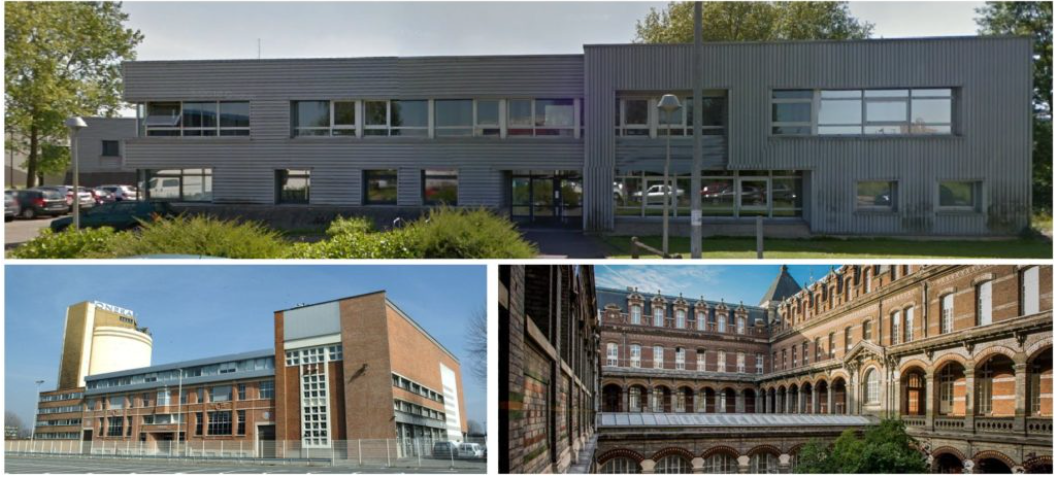
\includegraphics[scale=0.255]{../images/other/LMFL_facilities.png}
                \scriptsize Buildings of the Laboratoire de Mécanique des Fluides de Lille (LMFL)
            \end{column}
            \begin{column}{0.35\textwidth}
                \begin{enumerate}
                    \item Centrale Lille
                    \item Université de Lille
                    \item Arts et Métiers (ENSAM)
                    \item ONERA
                    \item CNRS
                \end{enumerate}

                \vspace{1cm}

                \begin{itemize}
                    \item 25 doctoral students
                    \item 38 permanent researchers
                \end{itemize}
            

            \end{column}
        \end{columns}
    \end{frame}

    \begin{frame}[t]{Corporate Social Responsibility (CSR)}
        \vspace{-0.5cm}
        \center
        \textbf{ENSAM action plan :}
        \begin{itemize}
            \item Strategy, governance and territorial anchoring
            \item Education and training -> eco-responsibility
            \item Research and innovation free access
            \item Environmental management
            \item Social policy
        \end{itemize}

        \vspace{0.3cm}

        \textbf{LMFL action plan :}
        \begin{itemize}
            \item Haut Conseil de l'Évaluation de la Recherche et de l'Enseignement Supérieur (HCERES)
            \item Unique facilities
            \item European laboratories in the field of next-generation aircraft design
            \item Advanced numerical simulations (turbulence) and data-driven modeling
            \item Synergy between geographically separated sites
            \item High quality of scientific output (JFM)
        \end{itemize}



    \end{frame}

    \begin{frame}[t]{Laboratory and host site}%{Laboratoire et site d'acceuil}
        %\begin{columns}
            %\begin{column}{0.40\textwidth}
                \center
                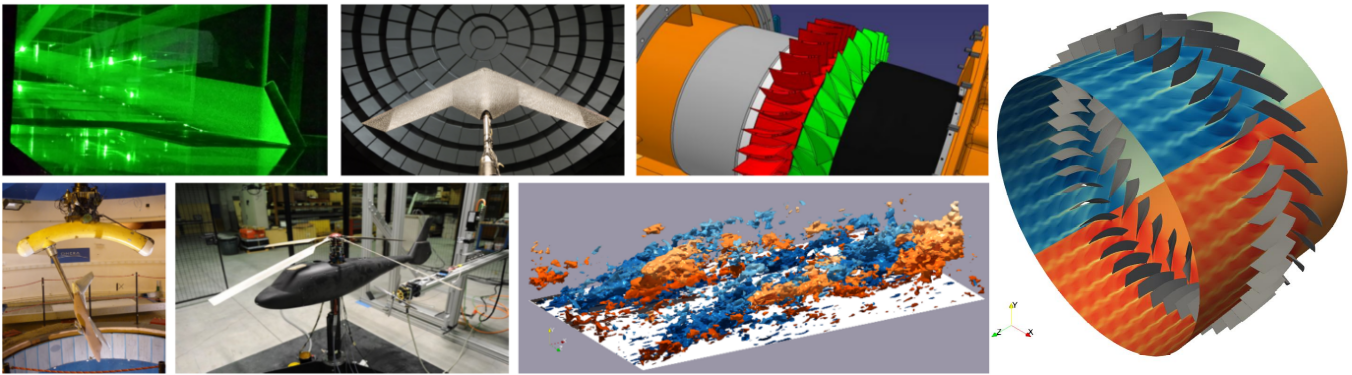
\includegraphics[scale=0.3]{../images/combo3.png}
                %\scriptsize Activitiées au LMFL
            %\end{column}
            %\begin{column}{0.60\textwidth}
                \vspace{-0.3cm}

                \begin{enumerate}
                    \item \textbf{Turbulence}
                    \item \textbf{Flight dynamics in an unsteady and inhomogeneous environment}%{Dynamique du vol en environnement instationnaire et inhomogène}
                    \item \textcolor{red}{\textbf{Rotating flows}}
                \end{enumerate}
            %\end{column}
        %\end{columns}
    \end{frame}

\begin{comment}
    
    \begin{frame}{Domaine d'expertise du LMFL à l'ENSAM}
        \begin{columns}
            \begin{column}{0.58\textwidth}
                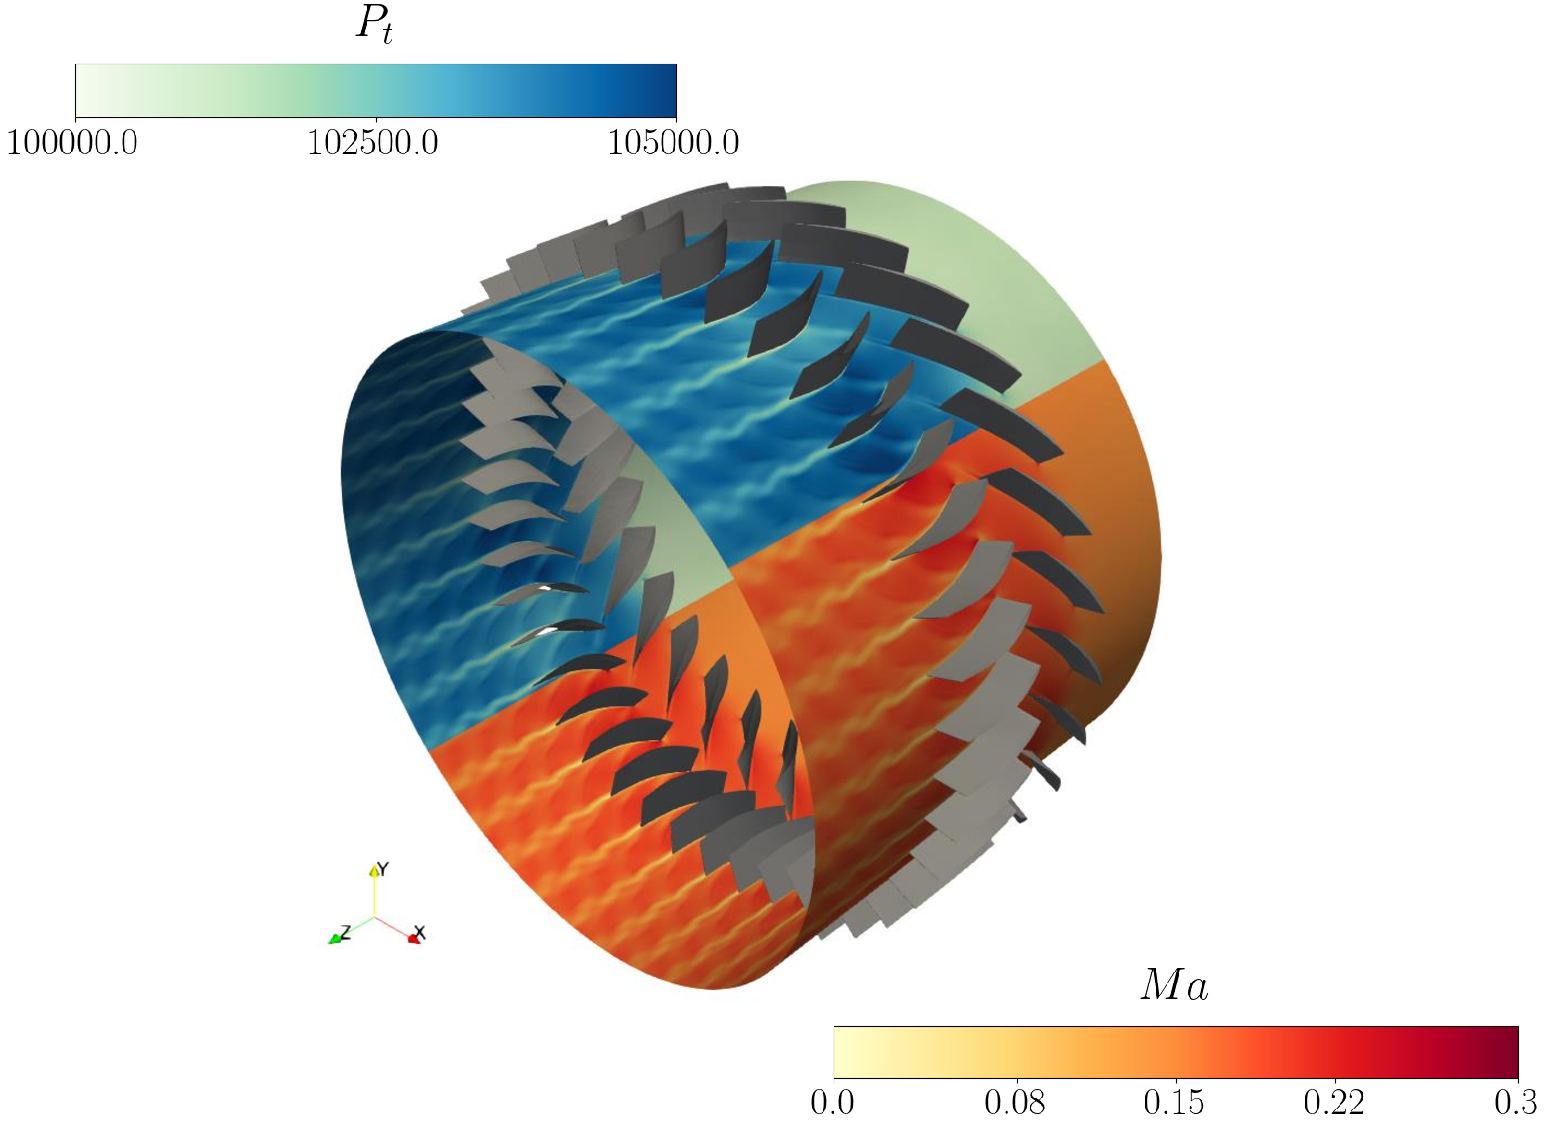
\includegraphics[scale=0.31]{../images/cme2.pdf}
                \scriptsize Simulation d'un écoulement dans un compresseur axial (CME2) \\ Tom MOUSSIE, LMFL - ENSAM
            \end{column}
            \begin{column}{0.42\textwidth}
                \begin{itemize}
                    \item Mécanique des fluides numérique
                    \item Ecoulements tourants
                    \item \textcolor{red}{Assimilation de données}
                \end{itemize}
            \end{column}
        \end{columns}
    \end{frame}
\end{comment}


    \begin{frame}{Data Assimilation in fluid mechanics}
        \vspace{-0.4cm}
        \begin{columns}[T] % T = top align
            % Colonne numérique
            \begin{column}{0.50\textwidth}
                \begin{block}{\textbf{Numerical simulation}}%{Simulation numérique}}
                    \begin{itemize}
                        \item Full field (velocity , pressures, etc.)
                        %\item Peu coûteux une fois le modèle construit
                        \baditem Limited accuracy (turbulence, mesh, boundary conditions, etc.)
                    \end{itemize}
                \end{block}
            \end{column}

            % Colonne expérimental
            \begin{column}{0.50\textwidth}
                \begin{block}{\textbf{Experimental}}%{Expérimentale}}
                    \begin{itemize}
                        \item Real and accurate measurements%Mesures réelles et précises
                        \item Essential validation of models%Validation indispensable des modèles
                        \baditem Local data, high cost and implementation%Données locales, coût et mise en place élevés
                    \end{itemize}
                \end{block}
            \end{column}
        \end{columns}

        %\vspace{0.3cm} % réduit pour remonter les deux du dessus
        \centering
        \begin{block}{\textbf{Data Assimilation}}%{Assimilation de données}}
            \textbf{Merge} numerical simulation and experimental data to obtain a more reliable and robust prediction.
            %Combiner \textbf{numérique} (complet mais approximatif) et \textbf{expérimental} (précis mais limité) 
            %pour obtenir des simulations plus fiables et robustes.
        \end{block}

        \centering
        %\begin{block}{\textbf{Difficultés du cas test de la pompe centrifuge}}
        \begin{block}{\textbf{Complexities of the centrifugal pump test case}}
            \textbf{Turbulent flow} around a \textbf{complex geometry} in \textbf{rotation}. \\
            %\textbf{Écoulement turbulent} autour d'une \textbf{géométrie complexe} en \textbf{rotation}. \\
            \vspace{0.2cm}
            %\alert{Jamais encore étudié avec assimilation de données.}
            \alert{Never studied yet with data assimilation}
        \end{block}
            

    \end{frame}

\begin{comment}
    \begin{frame}{Sujet du stage}
        \begin{columns}[t] % Alignement en haut
            % Colonne gauche
            \begin{column}{0.50\textwidth}
                % Titre + image pompe
                \begin{flushleft}
                    \textbf{Sujet du stage} : améliorer la performance d'une pompe centrifuge en utilisant des techniques d'assimilation de données (DA).
                    
                    \vspace{0.2cm}
                    \center
                    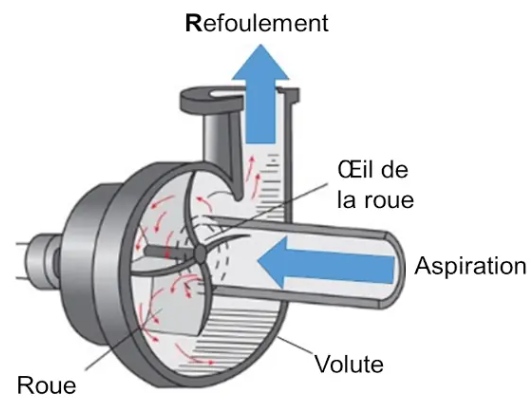
\includegraphics[scale=0.24]{../images/PompeCentrifuge.png} \\
                    \scriptsize Pompe centrifuge
                \end{flushleft}
                
                %\vfill
                
                % Image avion en bas

            \end{column}

            % Colonne droite
            \begin{column}{0.50\textwidth}
                \begin{flushleft}
                    \center
                    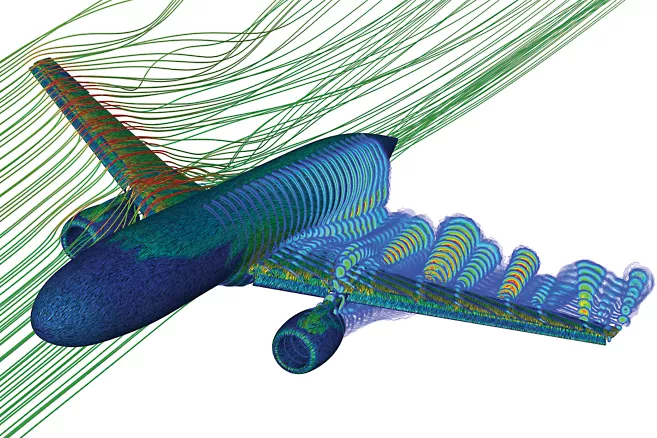
\includegraphics[scale=0.24]{../images/CFD.png} \\
                    \scriptsize Simulation Ansys Fluent d'une étude aérodynamique externe
                \end{flushleft}

                \vspace{0.3cm}

                \begin{itemize}
                    \item \textbf{Pompes centrifuges}
                    \item \textbf{Mécanique des fluides numérique}
                    \item \textbf{Optimisation de la performance}
                \end{itemize}
            \end{column}
        \end{columns}
    \end{frame}
\end{comment}

    
\begin{frame}{Sommaire}
    \tableofcontents   
\end{frame}


%%%%%%%%%%%%%%%%%%%%%%%%%%%%%%%%%%%%%%%%%%%%%%%%%%%%%%%%%%%%%%%%%%%%%%%%%%%%%%%%%%%%%%%%%%%%
\section{Cas test}

    \begin{frame}{Dispositif expérimental RESEDA}
        \center
        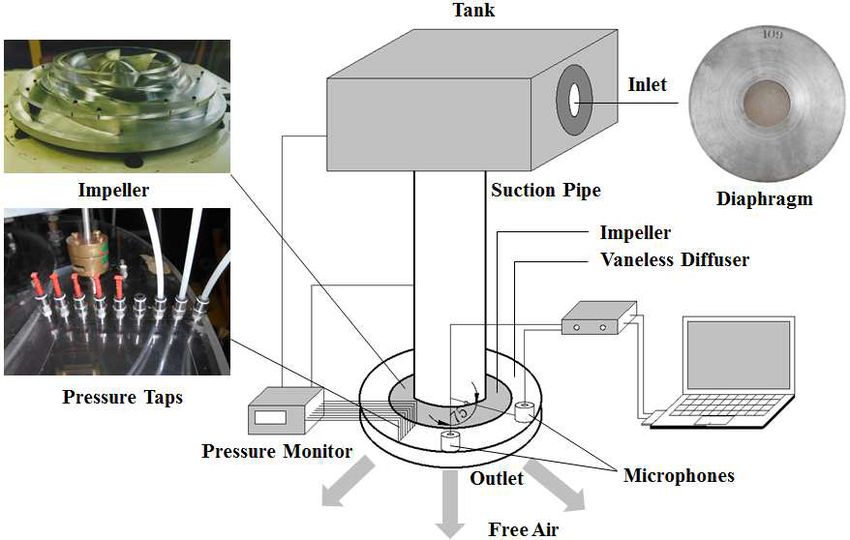
\includegraphics[scale=0.3]{../images/experimentalPump/setting_centrifugalPump.png}
        %\scriptsize Dispositif expérimental de la pompe centrifuge RESEDA

    \end{frame}
    

    \begin{frame}{Pompe centrifuge expérimentale}

        \begin{columns}
            \hspace{-0.1cm}
            \begin{column}{0.3\textwidth}
                %\begin{columns}
                    %\begin{column}{0.542\textwidth}
                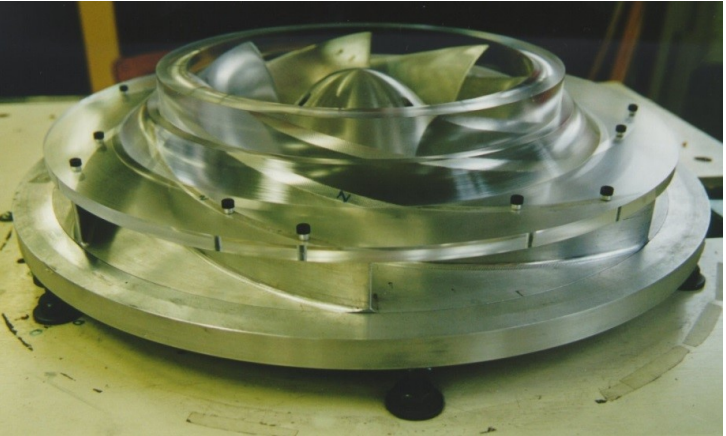
\includegraphics[scale=0.27]{../figures/RESEDA_benchmark.png}
                \scriptsize Roue à aubes de la pompe centrifuge RESEDA
                    %\end{column}
                    %\begin{column}{0.458\textwidth}
                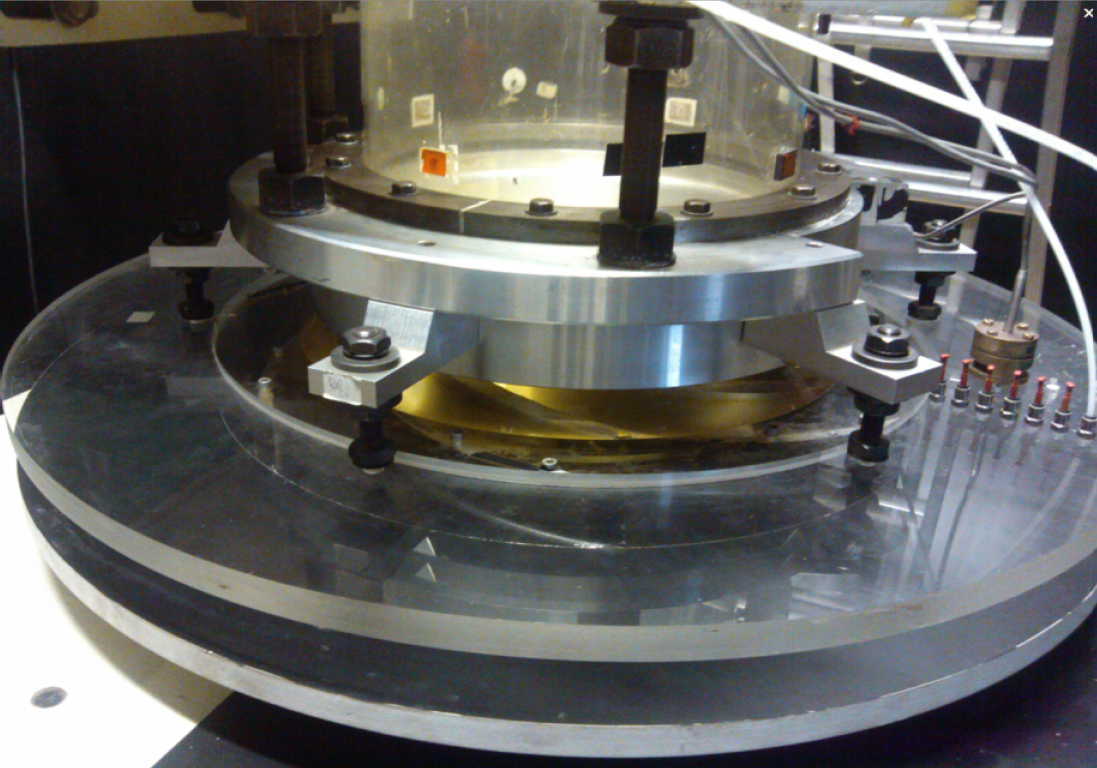
\includegraphics[scale=0.18]{../figures/image1.png}
                \scriptsize Roue à aubes dans le dispositif
                    %
            \end{column}
                %\end{columns}
            %\end{column}
            
            \begin{column}{0.28\textwidth}
                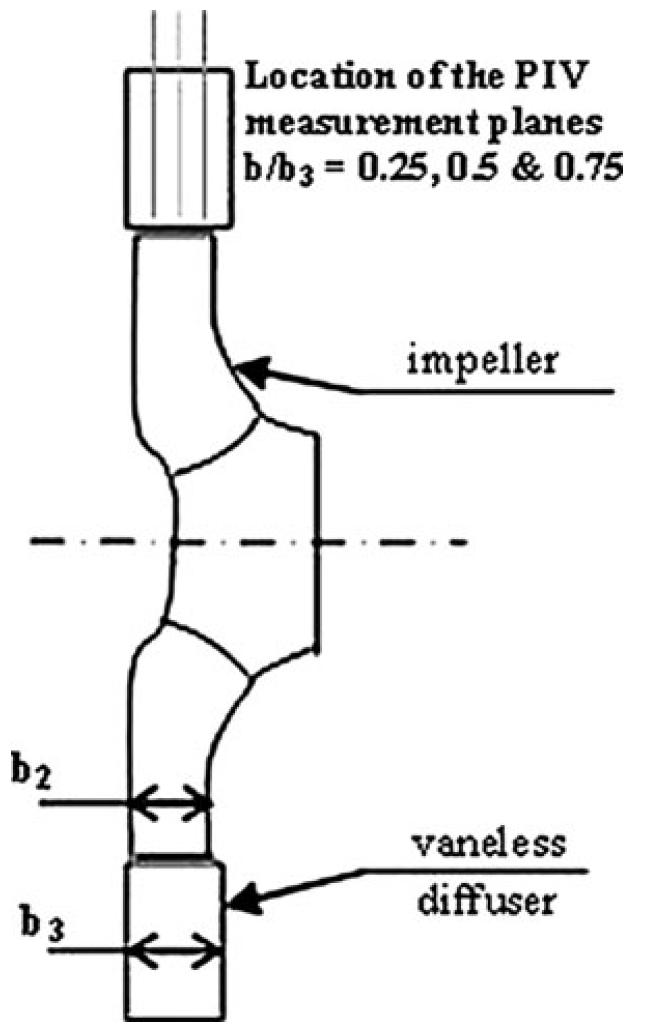
\includegraphics[scale=0.36]{../figures/impeller_position.png}
                \scriptsize \phantom{-} Position des plans PIV
            \end{column}
            \hspace{-1.5cm}
            \begin{column}{0.45\textwidth}
            \small{
                \begin{itemize}
                    \item $Re_\Omega=\cfrac{R_2^2 \Omega}{\nu} = 5.53\times10^5$ \textrm{\textbf{(turbulent)}}
                    \item $Ma = \cfrac{R_2 \Omega}{c} = 0.095$ \textrm{\textbf{(incompressible)}}
                    \item Point de fonctionnement nominal \[\frac{Q}{Q_d} = 1\]
                    \item Vitesse de rotation : 1 200 tr/min
                    \item 7 aubes
                    \item Données PIV à 980Hz
                \end{itemize}
            }
            %\hspace{-4cm}

            \end{column}

        \end{columns}

    \end{frame}

    \begin{frame}{Modèle numérique de la pompe centrifuge}
        \begin{columns}
            \begin{column}{0.49\textwidth}
                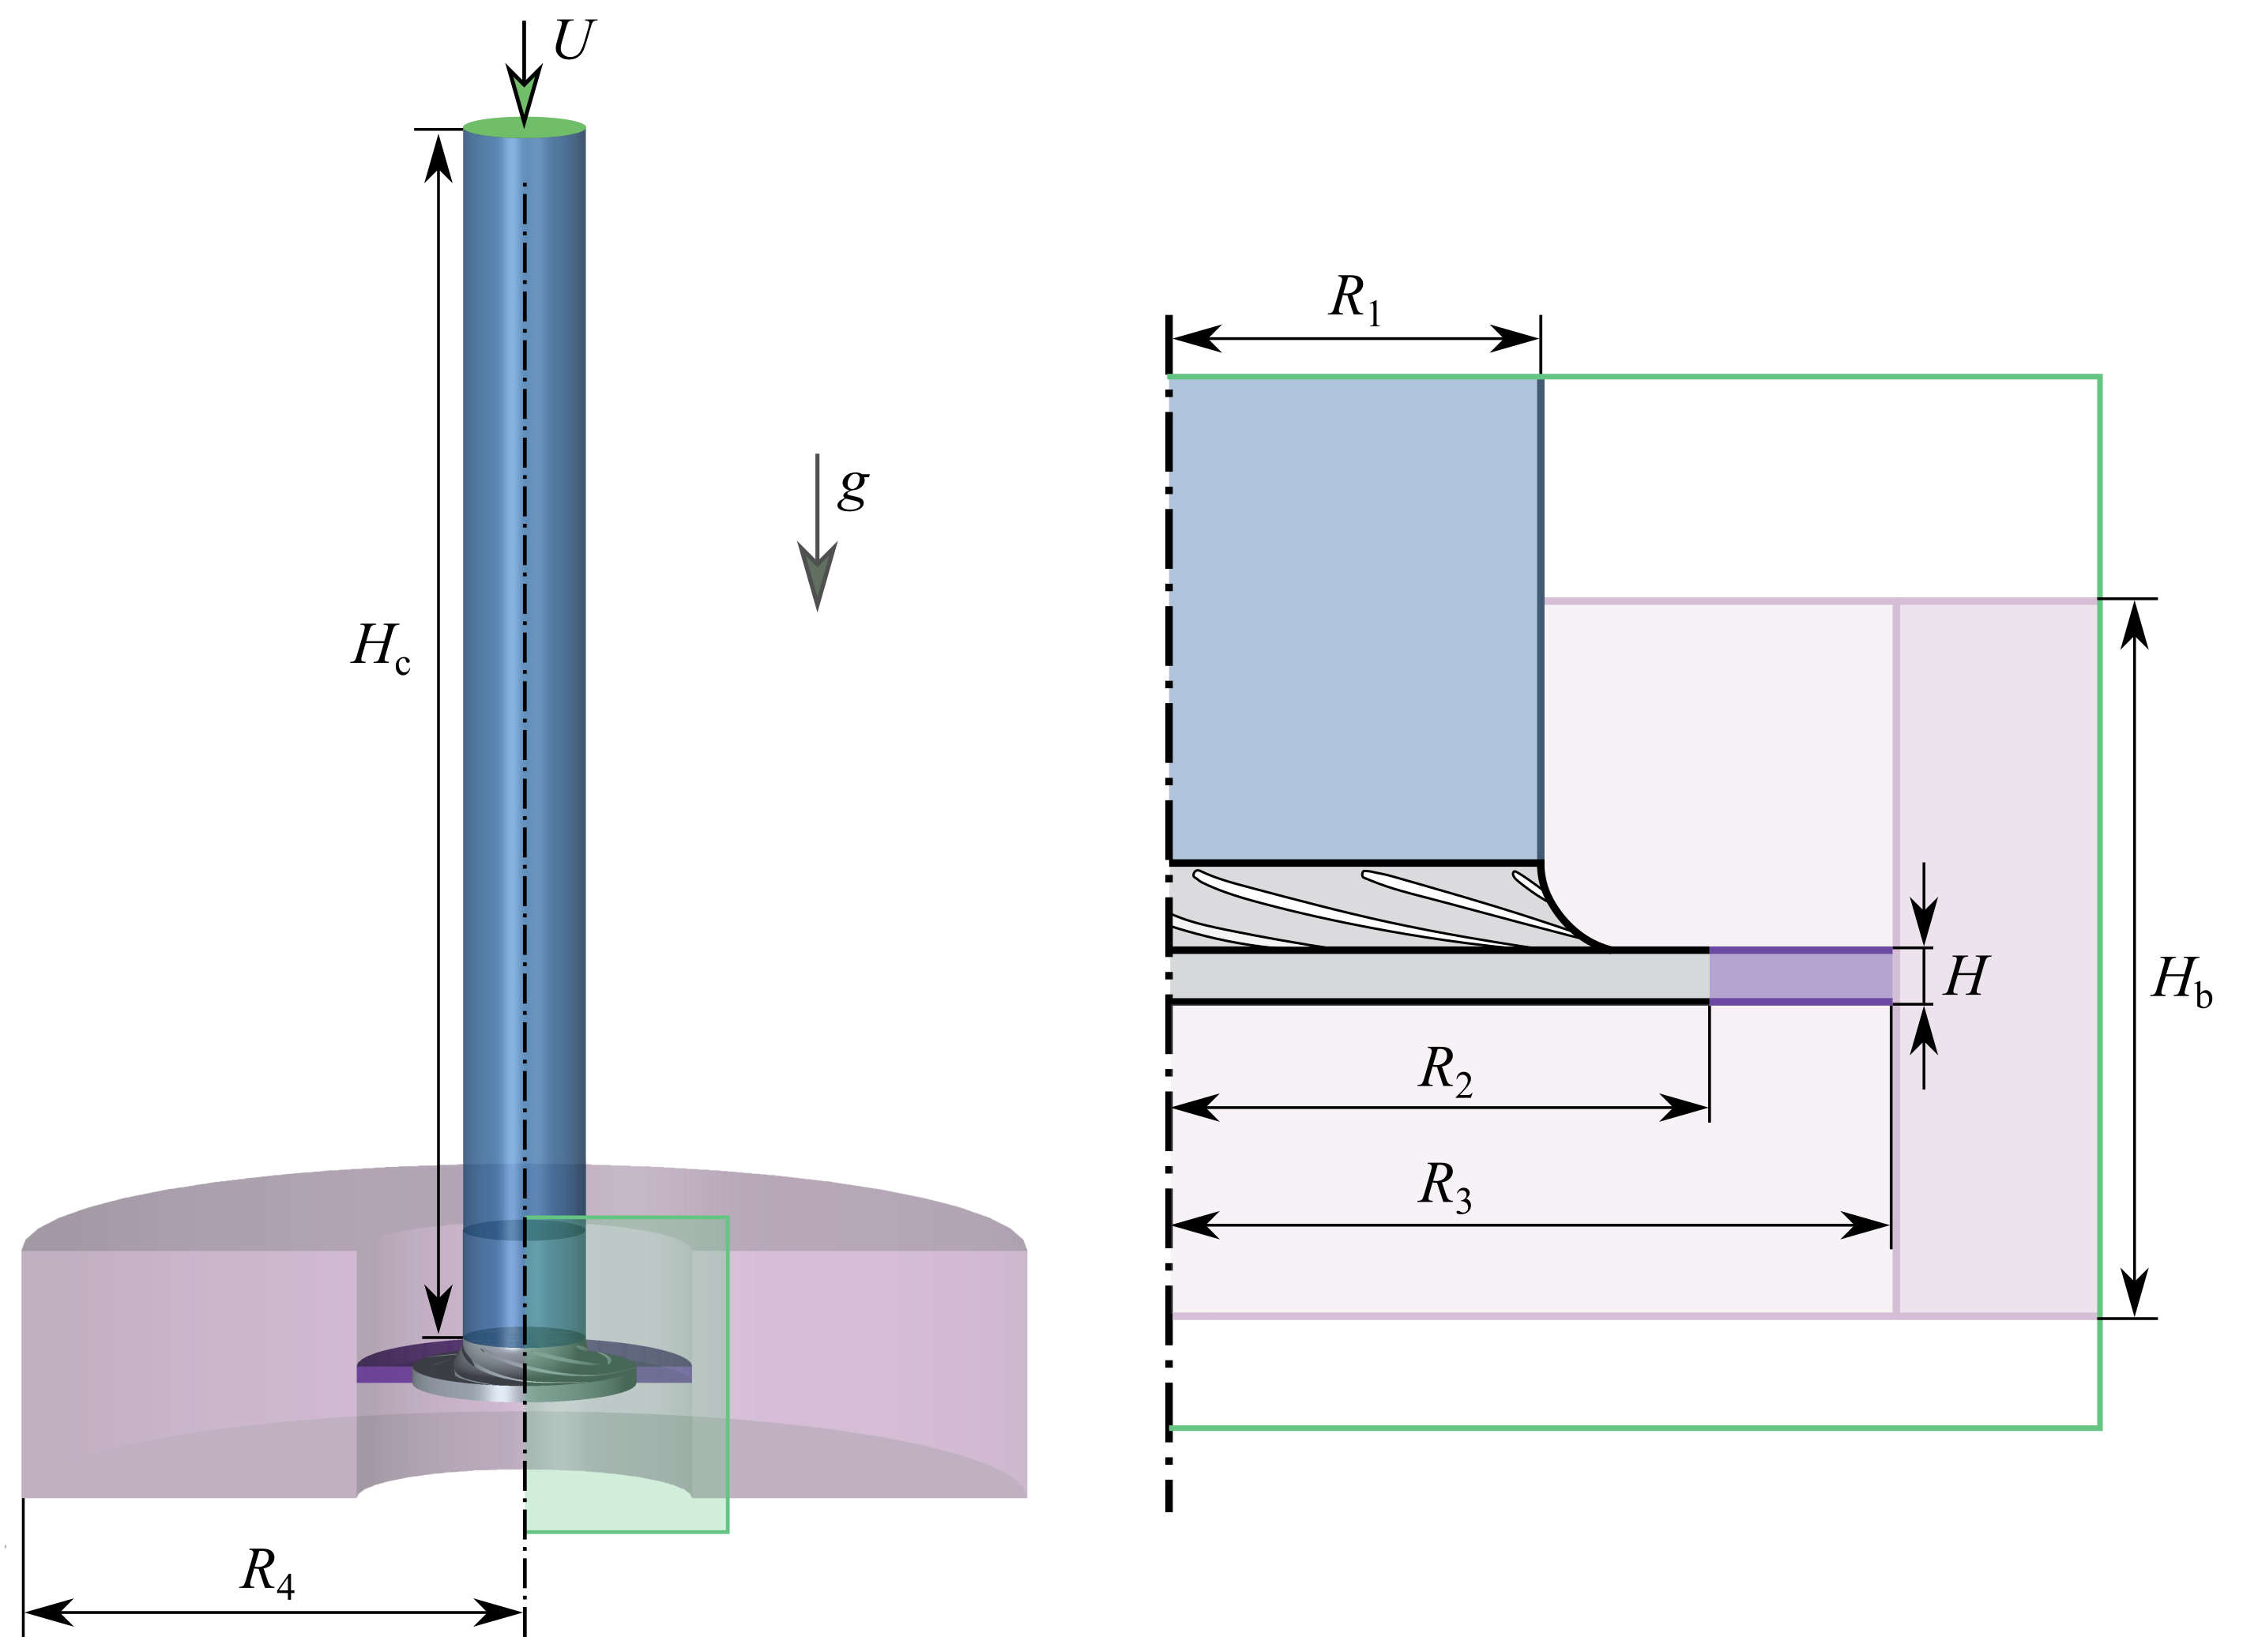
\includegraphics[scale=0.31]{../images/model/Sketch1.png} % ou RESEDA_sketch.pdf
                \scriptsize Modèle de la pompe centrifuge RESEDA
            \end{column}
            \begin{column}{0.52\textwidth}
                \begin{itemize}
                    \item 3 zones principales : entrée, roue, sortie
                    \item Fluide : air à 15\degree C
                    \item Vitesse en entrée : $U_{in} = 3.77$ m/s
                    \item Condition de pression en sortie : $p_{out} = 0$ Pa
                    \item 11 millions de cellules %structurées
                \end{itemize}   
            \end{column}
        \end{columns}       
    \end{frame}

    \begin{frame}{Modèle numérique de la pompe centrifuge} % Modélisation
        \begin{columns}
            \begin{column}{0.48\textwidth}
                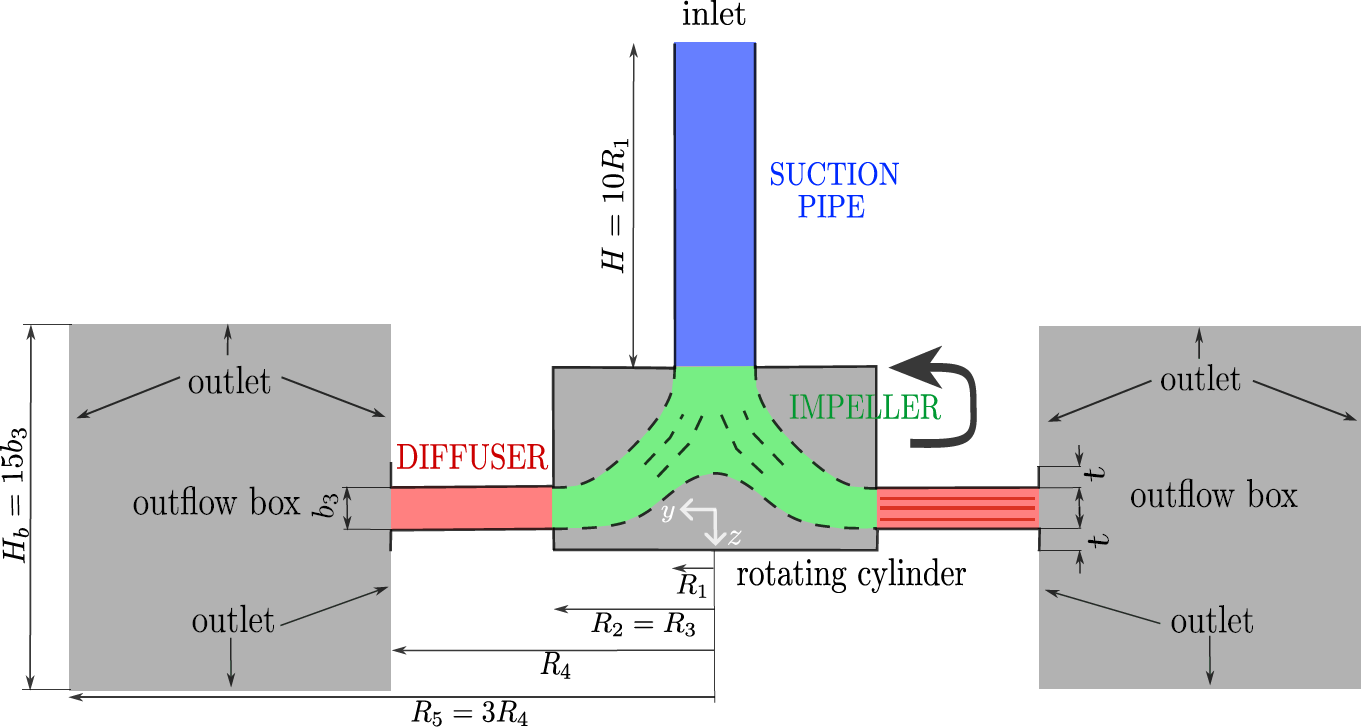
\includegraphics[scale=0.29]{../figures/RESEDA_sketchBisBis.png}
                \scriptsize Modèle de la pompe centrifuge RESEDA
                \footnotesize{\begin{itemize}
                    \item \textbf{Conditions aux limites :}
                        \begin{itemize}
                            \item Entrée $\rightarrow$ Vitesse%\texttt{flowRateInletVelocity}
                            \item Sortie $\rightarrow$ Pression%\texttt{fixedValue} (for the pressure $p$)
                        \end{itemize}
                    \item \textbf{IBM:} Appliquée au niveau de la roue %\structure{computational domain around the impeller}
                \end{itemize}}       
            \end{column}
            \hspace{1cm}
            \begin{column}{0.46\textwidth}
                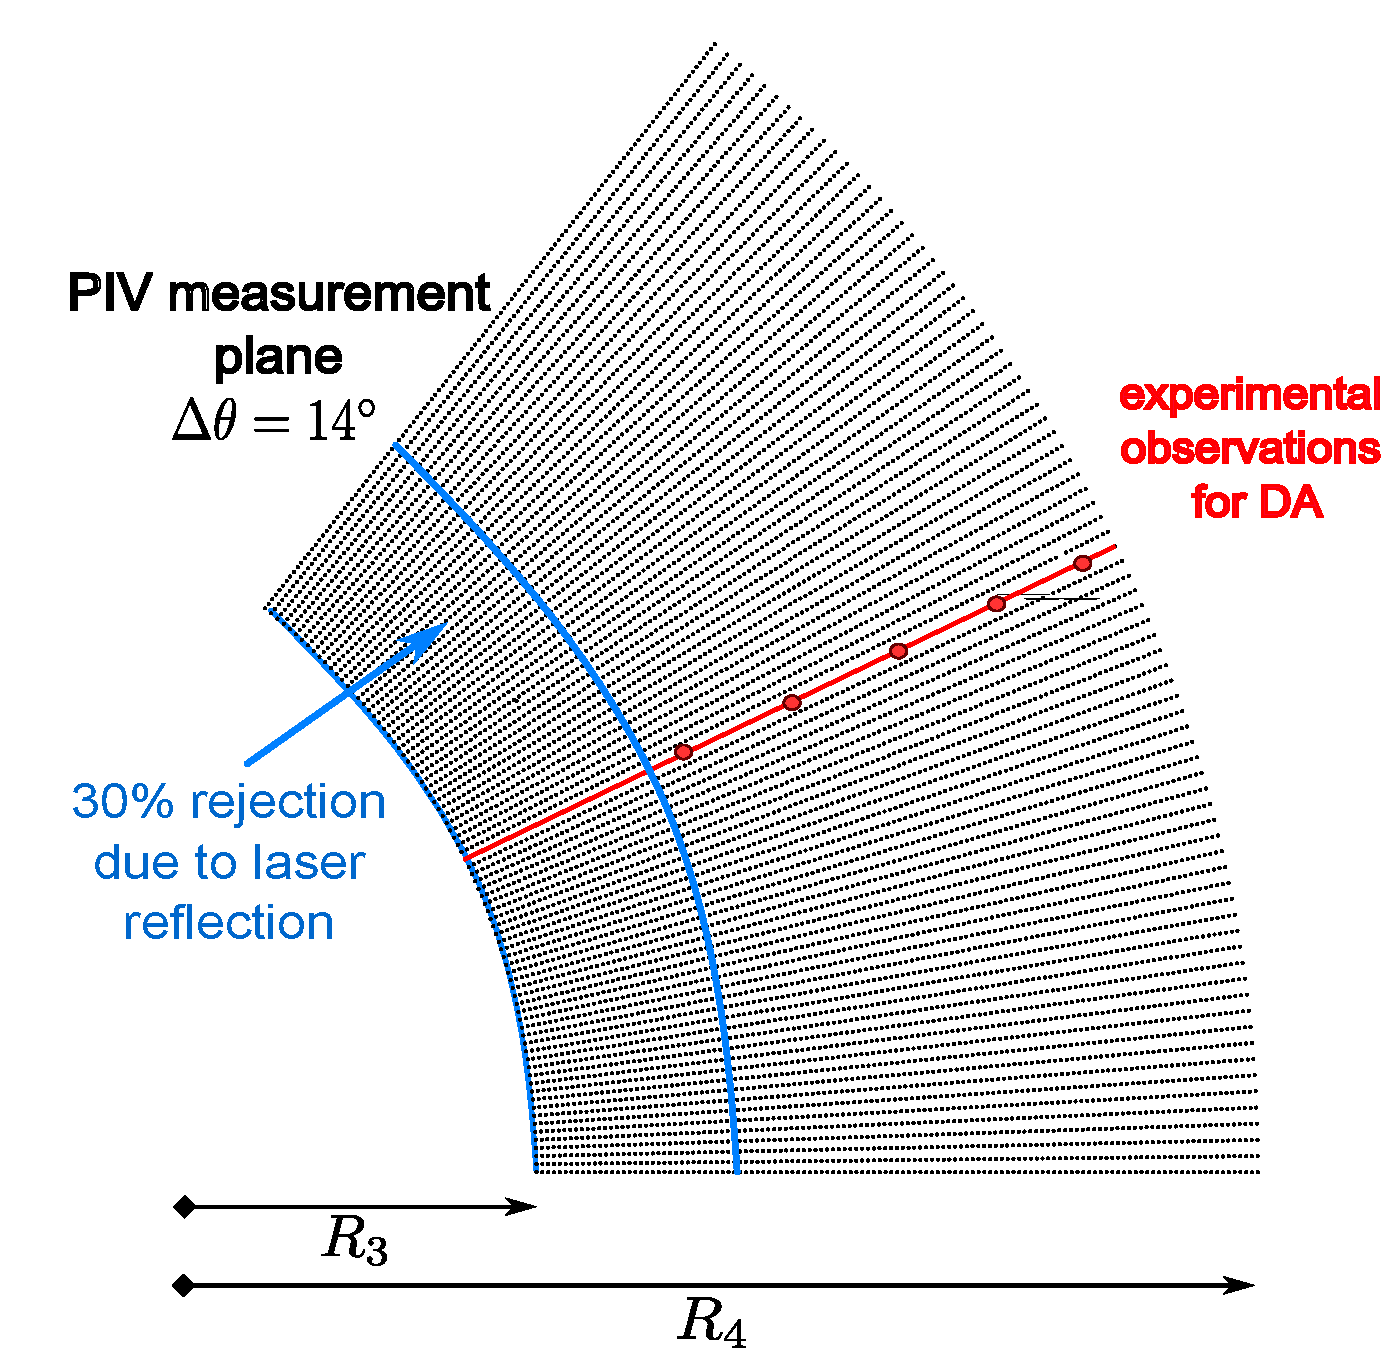
\includegraphics[scale=0.25]{../figures/polar_slice_avg_theta_trimmed.pdf}
                \scriptsize \phantom{-----} Mesures PIV moyennées azimutalement
            \end{column}
        \end{columns}
    \end{frame}

    \begin{frame}[t]{Étapes intermédiaires}

        \textbf{Sujet du stage} : améliorer la prédiction de la performance d'une pompe centrifuge en utilisant des techniques d'assimilation de données (DA)

        \vspace{1.2cm}

        \begin{itemize}
            \item Mise en avant des limitations de la méthode aux frontières immergées (IBM)
            \item Préparation des données expérimentales (PIV)
            \item Intégration d'algorithme d'assimilation de données
            \item Optimisation des paramètres de la méthode IBM
            %\item Valider les résultats obtenus par rapport aux données expérimentales.
        \end{itemize}
    \end{frame}

%%%%%%%%%%%%%%%%%%%%%%%%%%%%%%%%%%%%%%%%%%%%%%%%%%%%%%%%%%%%%%%%%%%%%%%%%%%%%%%%%%%%%%%%%%%%

    %\begin{frame}{Contexte et objectifs du stage}
    %\end{frame}


%%%%%%%%%%%%%%%%%%%%%%%%%%%%%%%%%%%%%%%%%%%%%%%%%%%%%%%%%%%%%%%%%%%%%%%%%%%%%%%%%%%%%%%%%%%%
\section{Outils numériques} 
%%%%%%%%%%%%%%%%%%%%%%%%%%%%%%%%%%%%%%%%%%%%%%%%%%%%%%%%%%%%%%%%%%%%%%%%%%%%%%%%%%%%%%%%%%%%

    \begin{frame}{La mécanique des fluides numérique}

        \begin{columns}[T]
            % --- Colonne gauche : équations et modèles ---
            \begin{column}{0.55\textwidth}
                \begin{block}{Équations de Navier–Stokes incompressibles}
                    \[
                    \text{Continuité : } \nabla \cdot \mathbf{u} = 0
                    \]
                    \[
                    \text{Moment : } \frac{\partial \mathbf{u}}{\partial t} + \mathbf{u}\cdot\nabla \mathbf{u}
                    = - \frac{\nabla p}{\rho} + \nu \nabla^2 \mathbf{u} + \boldsymbol{f}_P
                    \]
                \end{block}

                \begin{block}{Modèles numériques}
                    \begin{itemize}
                        \item Reynolds-Averaged Navier-Stokes (RANS)
                        \item Modèle de turbulence : \textbf{$\mathcal{K}-\omega$ SST}
                        \item Multiple Reference Frame (MRF)
                        \item Immersed Boundary Method (IBM)
                    \end{itemize}
                \end{block}
            \end{column}

            % --- Colonne droite : illustrations ---
            \begin{column}{0.45\textwidth}
                \begin{figure}
                    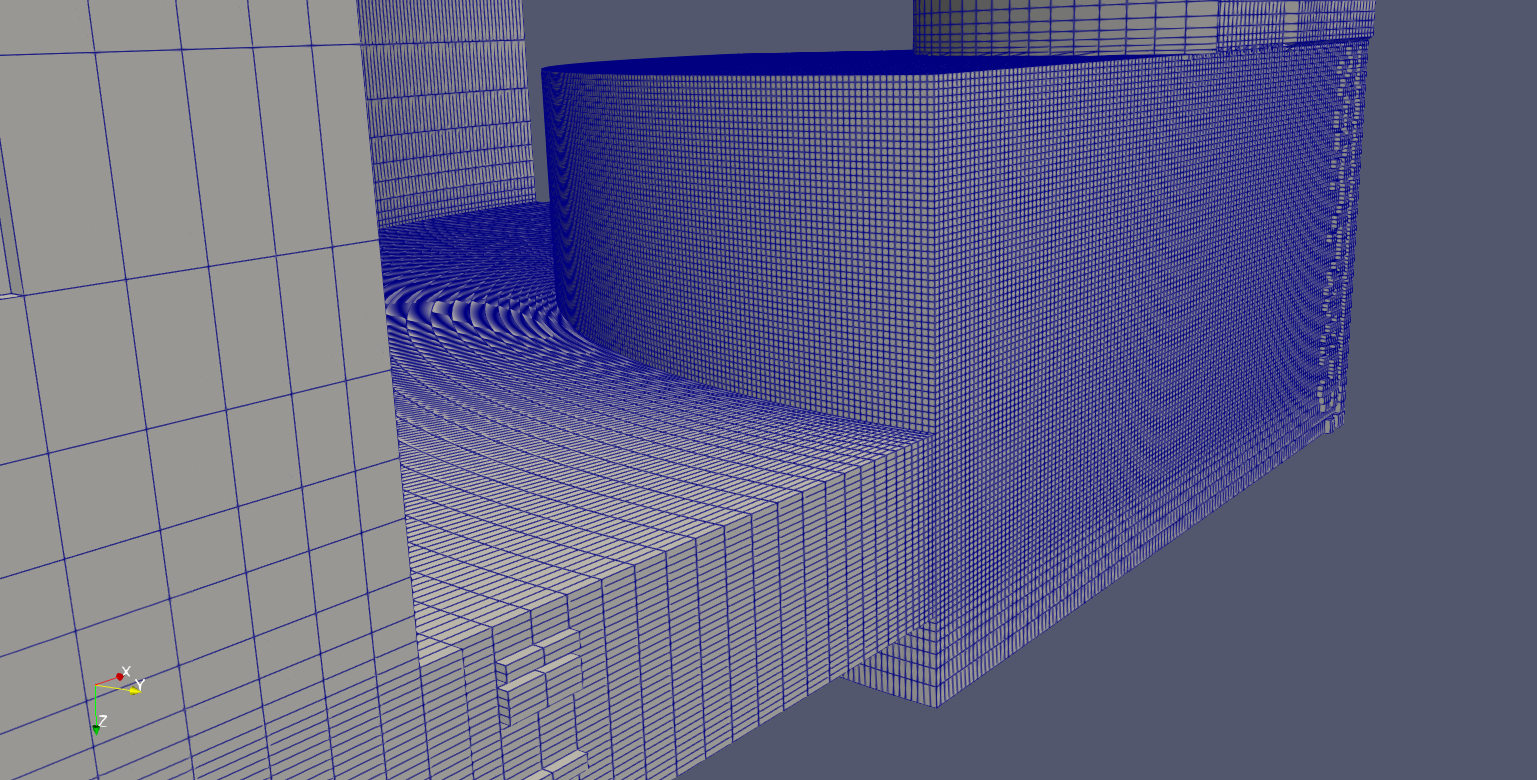
\includegraphics[width=0.79\textwidth]{../images/meshEx.png}\\  % -> discretisation
                    \scriptsize Exemple de maillage
                \end{figure}
                \vspace{-0.31cm}
                \begin{figure}
                    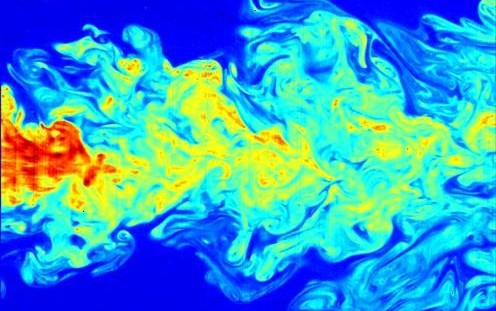
\includegraphics[width=0.65\textwidth]{../images/turbulence2.jpg}\\
                    \scriptsize Turbulence
                \end{figure}
            \end{column}
        \end{columns}

    \end{frame}

    \begin{frame}{Méthode aux frontières immergées}
        \begin{center}
            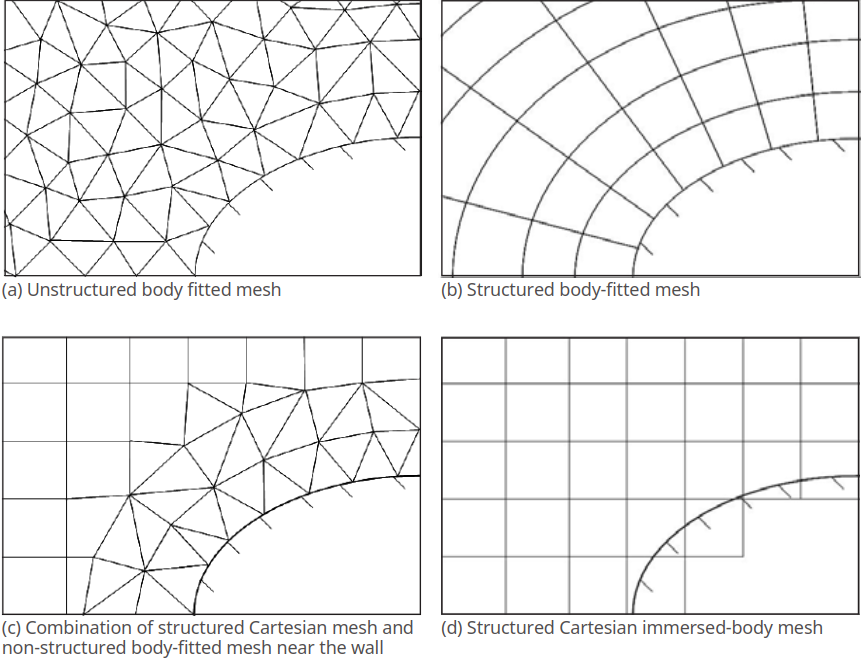
\includegraphics[scale=0.25]{../images/solidworksMesh3.png} \\
            \scriptsize Différence entre un maillage body-fitted classique et un maillage IBM
        \end{center}
    \end{frame}


    \begin{frame}{Méthode aux frontières immergées}

        \begin{block}{\texorpdfstring{\structure{\textbf{Penalisation IBM:}}}{Pénalisation IBM:}}
                Pénalisation continue de type IBM pour les écoulements incompressibles $\Rightarrow$ définition d'un \texorpdfstring{\structure{terme de forçage direct local}}{terme de forçage direct local} $\boldsymbol{f}_P$ dans les équations de Navier–Stokes, afin d'\textbf{imposer les conditions aux limites sur la paroi immergée} $\boldsymbol{(ib)}$.
        \end{block}

        \vspace{-0.2cm}

%\begin{equation*}
%\rho\,\boldsymbol{\nabla} \cdot (\boldsymbol{u} \otimes \boldsymbol{u}) = -\boldsymbol{\nabla} p + \mu\, \nabla^2 \boldsymbol{u} \; \overbrace{-\,\chi\, \mu\, D \left(\boldsymbol{u} - \boldsymbol{u}_{ib} \right)}^{\boldsymbol{f}_P}
%\end{equation*}

        \begin{columns}
            \begin{column}{0.5\textwidth}
                \centering
                \begin{equation*}
                    (\boldsymbol{u} \cdot \boldsymbol{\nabla})\, \boldsymbol{u} = 
                    -\frac{1}{\rho} \nabla p + \nu \nabla^2 \boldsymbol{u} 
                    \underbrace{- \xi \nu \boldsymbol{D} \left( \boldsymbol{u} - \boldsymbol{u}_{ib} \right)}_{\boldsymbol{f}_P}
                \end{equation*}

                \vspace{-0.3cm}

                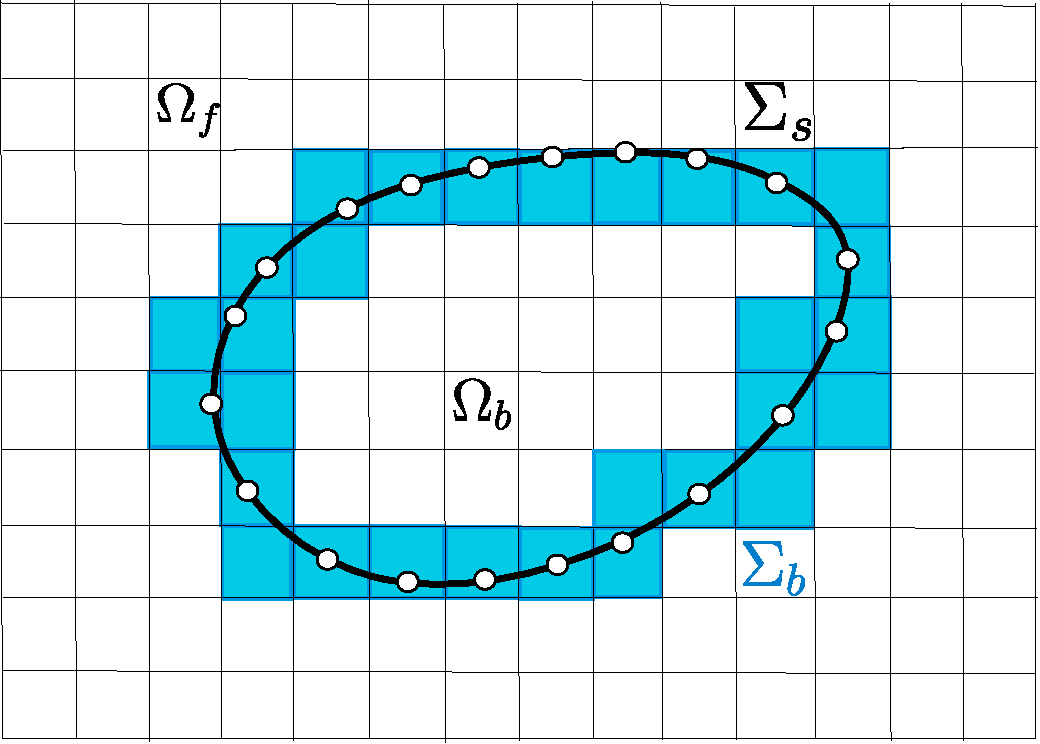
\includegraphics[scale=0.20]{../figures/IBM_Mesh.pdf}
                %\only<1>{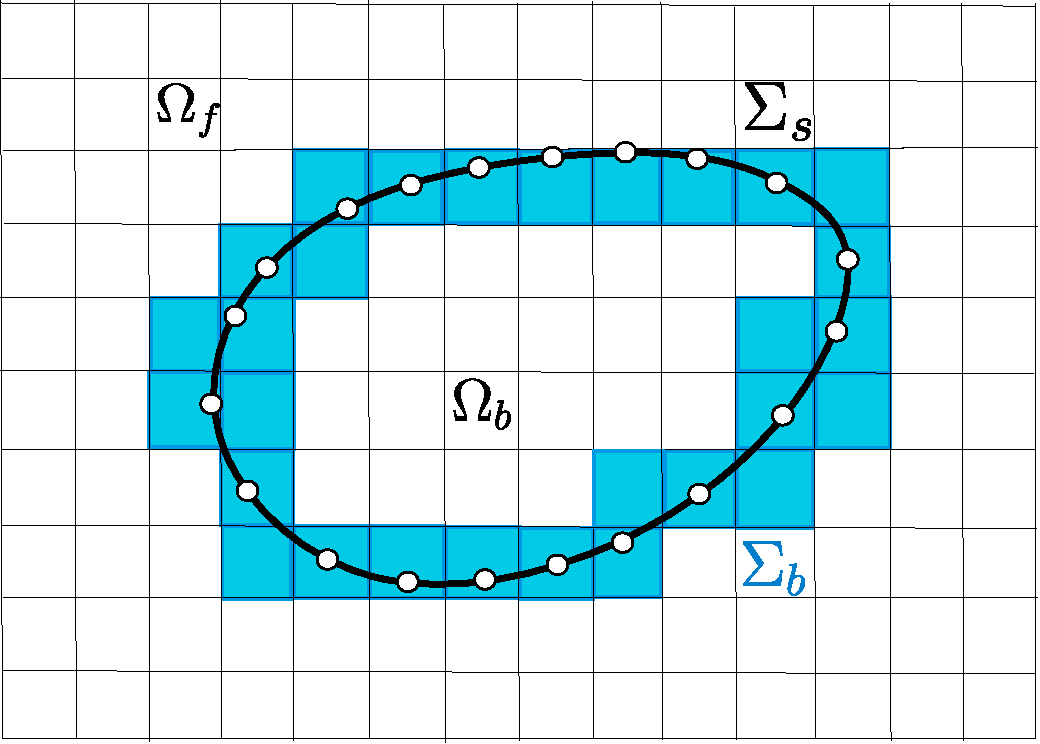
\includegraphics[scale=0.25]{../figures/IBM_Mesh.pdf}}
                %\only<2>{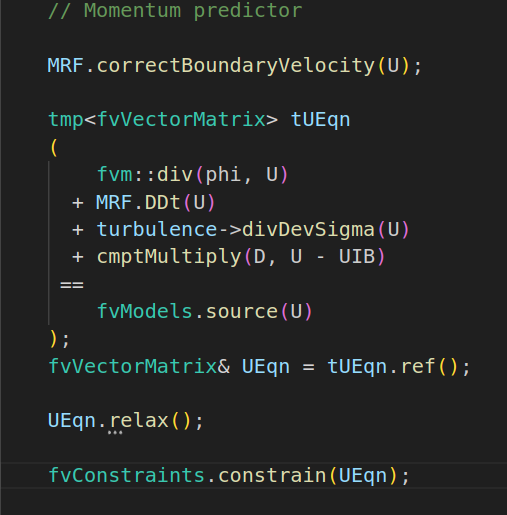
\includegraphics[scale=0.25]{../figures/implicit_forcing.png}}
            \end{column}
            \begin{column}{0.5\textwidth}
                %avec $[p] = M \cdot L^{-1} \cdot T^{-2}$
                \begin{equation*}
                    \xi = \left\{
                    \begin{array}{ll}
                        0 & \textrm{if } \boldsymbol{x} \in \Omega_f \\
                        1 & \textrm{if } \boldsymbol{x} \in (\Sigma_b \cup \Omega_b)
                    \end{array} \right.
                \end{equation*}

                \colorbox{blue!20}
                {\parbox{0.85\textwidth}
                { \centering Quand $D \rightarrow \infty$, \\ \textbf{champ IBM = champ body-fitted }}}

                \vspace{0.2cm}
                
                \footnotesize{... mais des valeurs trop élevées de $D$ peuvent mener à des instabilités...}
                
            \end{column}
        \end{columns}
        
    \end{frame}

    \begin{frame}{Le filtre de Kalman d'ensemble}
        \center
        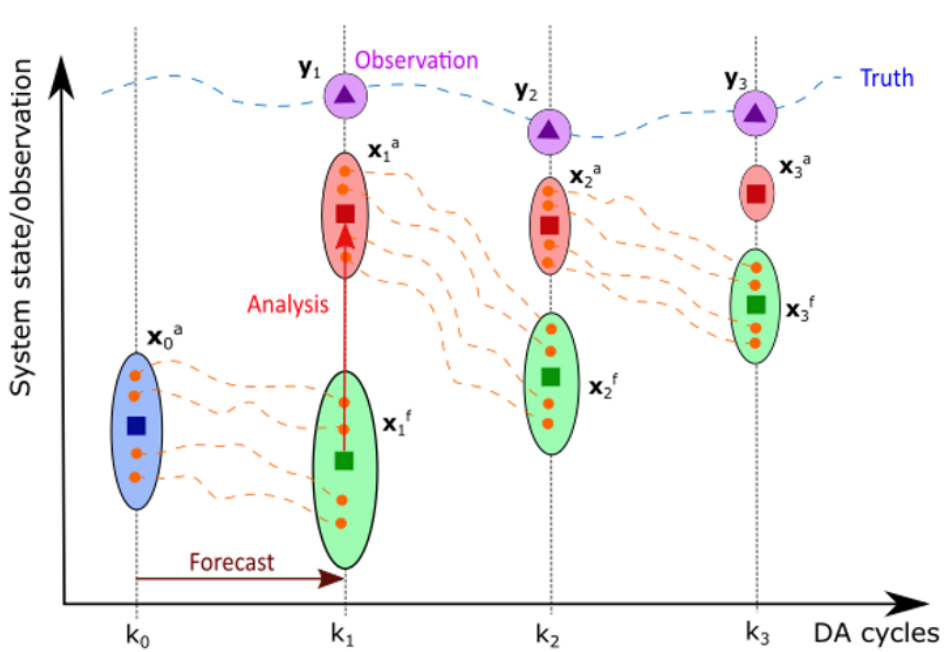
\includegraphics[scale=0.25]{../images/enkf_shem.png} % ou RESEDA_sketch.pdf
        %\scriptsize Schéma de principe de l'EnKF
    \end{frame}

    \begin{frame}
        \frametitle{{\small \centering Coupling OpenFOAM with Numerical EnvironmentS}}
        \begin{center}
            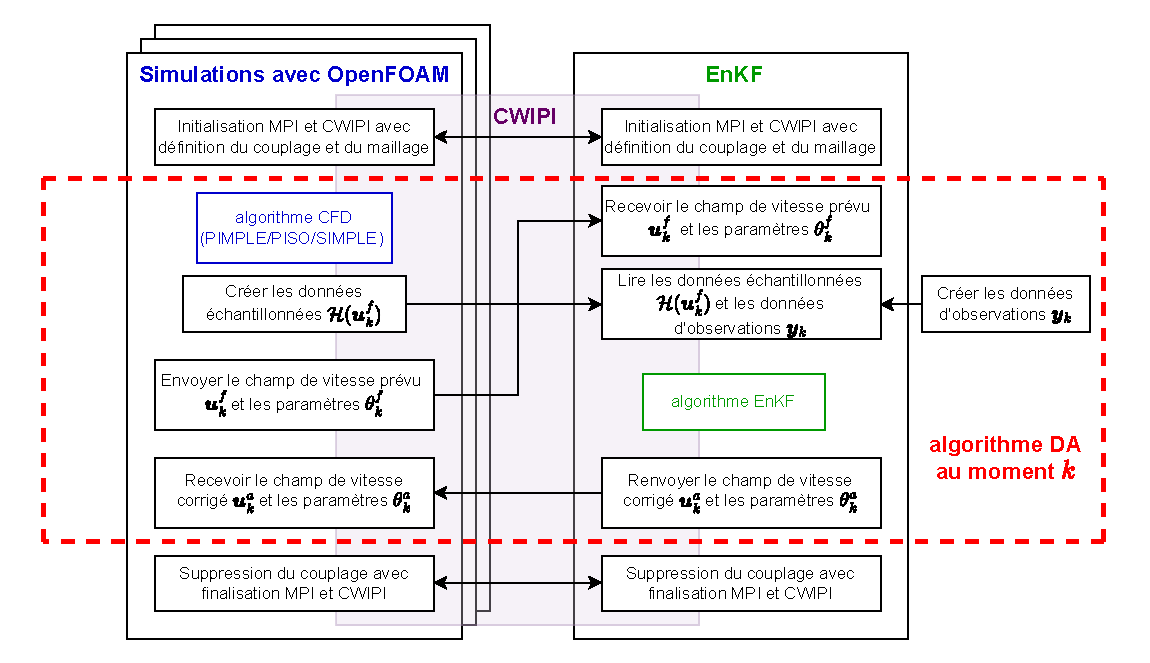
\includegraphics[scale=0.56]{../images/EnKF_Cones_français.pdf} % ou RESEDA_sketch.pdf
            %\scriptsize Schéma de principe de Coupling OpenFOAM with Numerical EnvironmentS (CONES)
        \end{center}
    \end{frame}


%%%%%%%%%%%%%%%%%%%%%%%%%%%%%%%%%%%%%%%%%%%%%%%%%%%%%%%%%%%%%%%%%%%%%%%%%%%%%%%%%%%%%%%%%%%%
\section{Applications et résultats} 
%%%%%%%%%%%%%%%%%%%%%%%%%%%%%%%%%%%%%%%%%%%%%%%%%%%%%%%%%%%%%%%%%%%%%%%%%%%%%%%%%%%%%%%%%%%%

    \begin{frame}{Assimilation de données avec EnKF}

        \begin{columns}[T]
        % Partie modèle
            \begin{column}{0.45\textwidth}
                \begin{block}{\textbf{Modèle}}
                \begin{itemize}
                    \item 30 simulations (RANS, k-$\omega$ SST)
                    \item OpenFOAM
                    \item IBM
                \end{itemize}
                \end{block}
            \end{column}

        % Partie observations
            \begin{column}{0.45\textwidth}
                \begin{block}{\textbf{Observations}}
                \begin{itemize}
                    \item Données expérimentales pompe
                    \item 45 vitesses $u$, pression $p$
                \end{itemize}
                \end{block}
            \end{column}
        \end{columns}

    \vspace{0.5cm}

    \centering
    \textbf{Objectif :} Combiner CFD + expérimental pour optimiser les coefficients $\boldsymbol{D_u}, D_\mathcal{K}, D_\omega$
    
    \vspace{1cm}

        \centering
            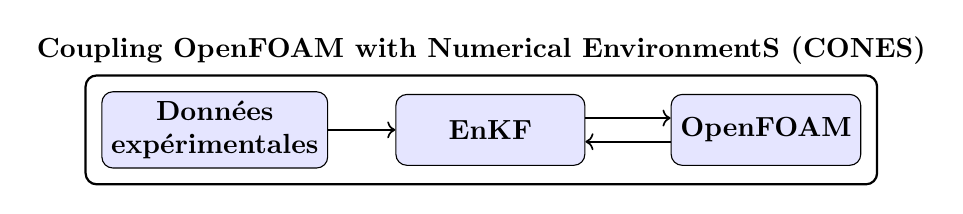
\begin{tikzpicture}[
                    box/.style={
                        draw,
                        rounded corners,
                        minimum width=2.4cm,
                        minimum height=0.9cm,
                        align=center,
                        font=\bfseries,
                        fill=blue!10
                    },
                    arrow/.style={
                        ->,
                        semithick
                    },
                    bigbox/.style={
                        draw,
                        rounded corners,
                        thick,
                        inner sep=0.2cm,
                        label={[font=\bfseries]above:Coupling OpenFOAM with Numerical EnvironmentS (CONES)}
                    }
                ]

                % Ligne principale
                \node[box] (data) at (0,0) {Données \\ expérimentales};
                \node[box] (enkf) at (3.5,0) {EnKF};
                \node[box] (openfoam) at (7,0) {OpenFOAM};

                % Flèches horizontales
                \draw[arrow] (data.east) -- (enkf.west);
                \draw[arrow] ([yshift=+0.15cm]enkf.east) -- ([yshift=+0.15cm]openfoam.west);
                \draw[arrow] ([yshift=-0.15cm]openfoam.west) -- ([yshift=-0.15cm]enkf.east);

                % Gros cadre "CONES"
                \node[bigbox, fit=(data)(enkf)(openfoam)] {};

            \end{tikzpicture}

    \vspace{0.3cm}

    \end{frame}




    \begin{frame}{Modélisation IBM}

        \begin{columns}
            \hspace{-0.5cm}
            \begin{column}{0.5\linewidth}
            \begin{itemize}[<+->]
                \item Simulation stationnaire % avec l'approche \texorpdfstring{\structure{\textbf{Multiple Reference Frame (MRF)}}}{Multiple Reference Frame (MRF)}
                \item Modèle de turbulence $\mathcal{K}-\omega$ SST $\rightarrow$ 
                Cinq coefficients de pénalisation 
                $D = (\textcolor{red}{\boldsymbol{D_u}}, \textcolor{red}{D_\mathcal{K}}, \textcolor{red}{D_\omega})$

                

            \begin{align*}
                \boldsymbol{f}_{P_{\boldsymbol{u}}} = \xi \nu \textcolor{red}{\boldsymbol{D_u}} (\boldsymbol{u}-\boldsymbol{u_{ib}}) \quad \rightarrow \boldsymbol{u_{ib}} &= \cancel{\boldsymbol{u}_r} + \boldsymbol{\Omega} \times \boldsymbol{r} \\
                \boldsymbol{f}_{P_\mathcal{K}} = \xi \nu \textcolor{red}{D_{\mathcal{K}}} (\mathcal{K}-\mathcal{K}_{ib}) \quad \rightarrow \mathcal{K}_{ib} &= 0 \\
                \boldsymbol{f}_{P_\omega} = \xi \nu \textcolor{red}{D_{\omega}} (\omega-\omega_{ib}) \quad \rightarrow \omega_{ib} &= (\omega_{vis}^2+\omega_{log}^2)^{1/2}
            \end{align*}
            où $\omega_{vis}=\frac{6 \nu}{\beta_1 y_{\mathrm{ref}}^2}$ et $\omega_{log} = \frac{\sqrt{\mathcal{K}}}{C_\mu \kappa y_\mathrm{ref}}$

            \vspace{0.5cm}

            %\centering
            %\texttt{kOmegaSST\_penalization}

            \end{itemize}

            \end{column}
            \begin{column}{0.5\linewidth}
                \centering
                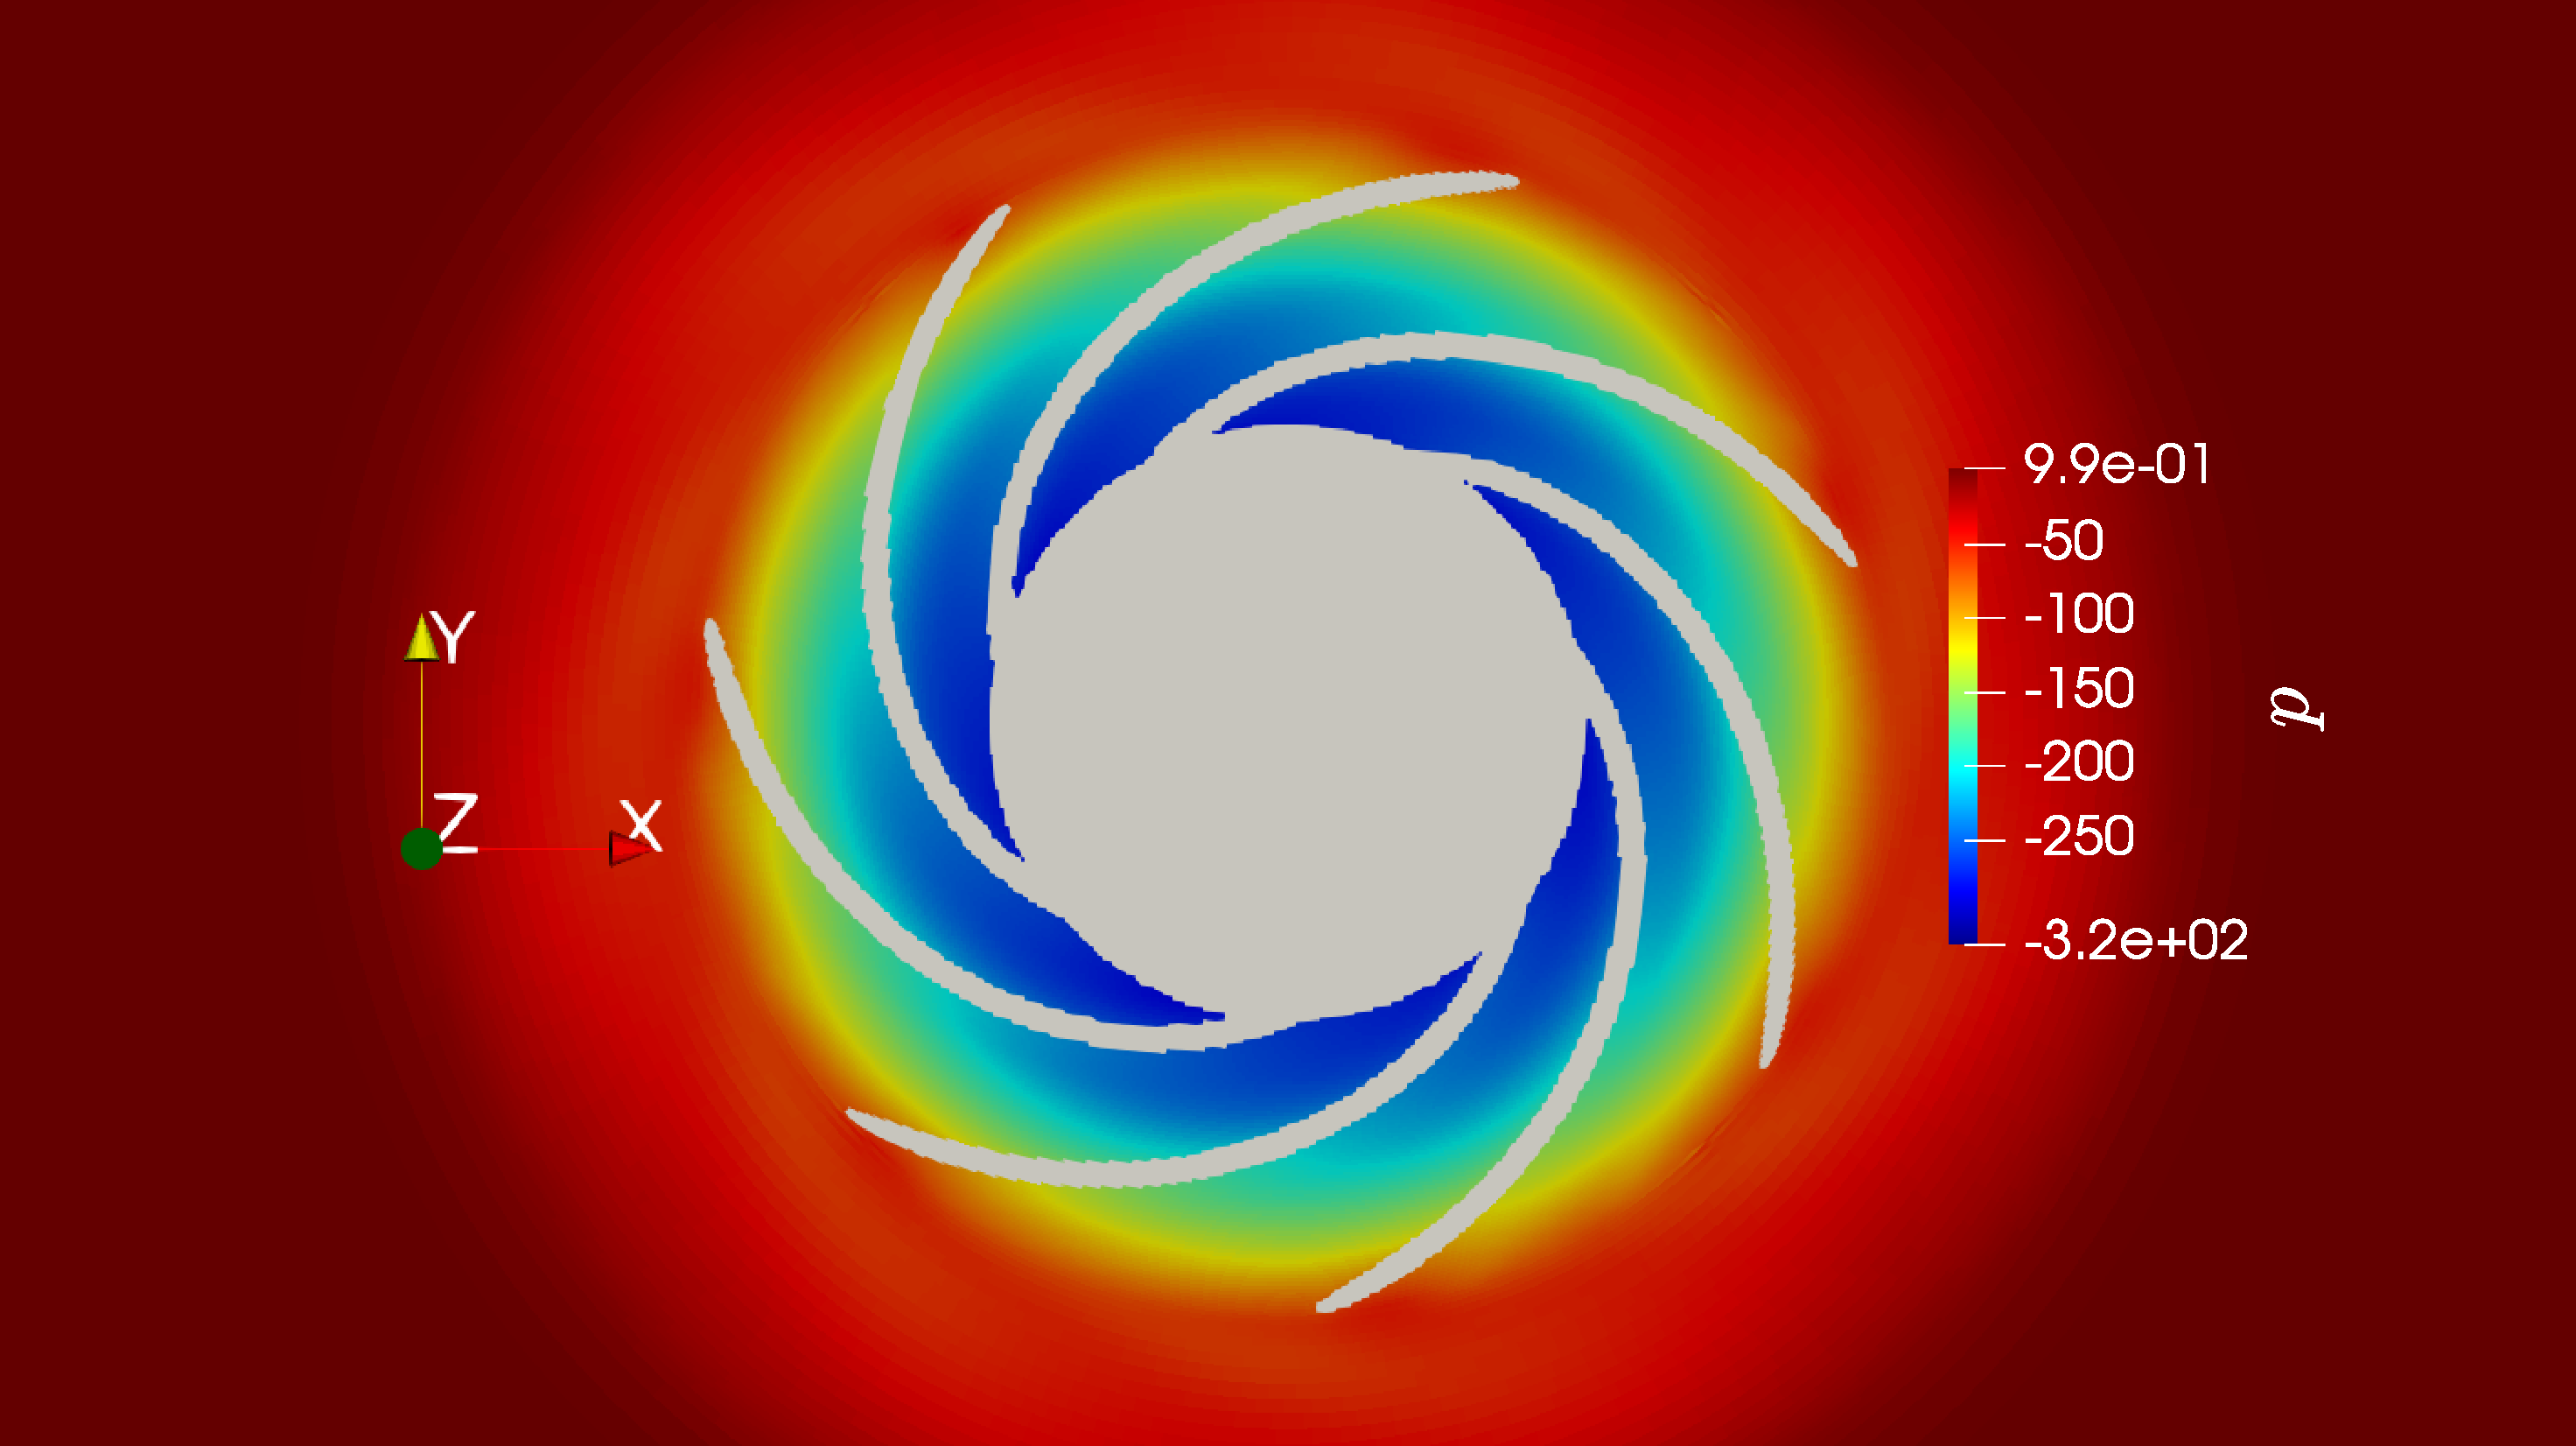
\includegraphics[width=0.8\textwidth]{../figures/pressure_profile.pdf}
                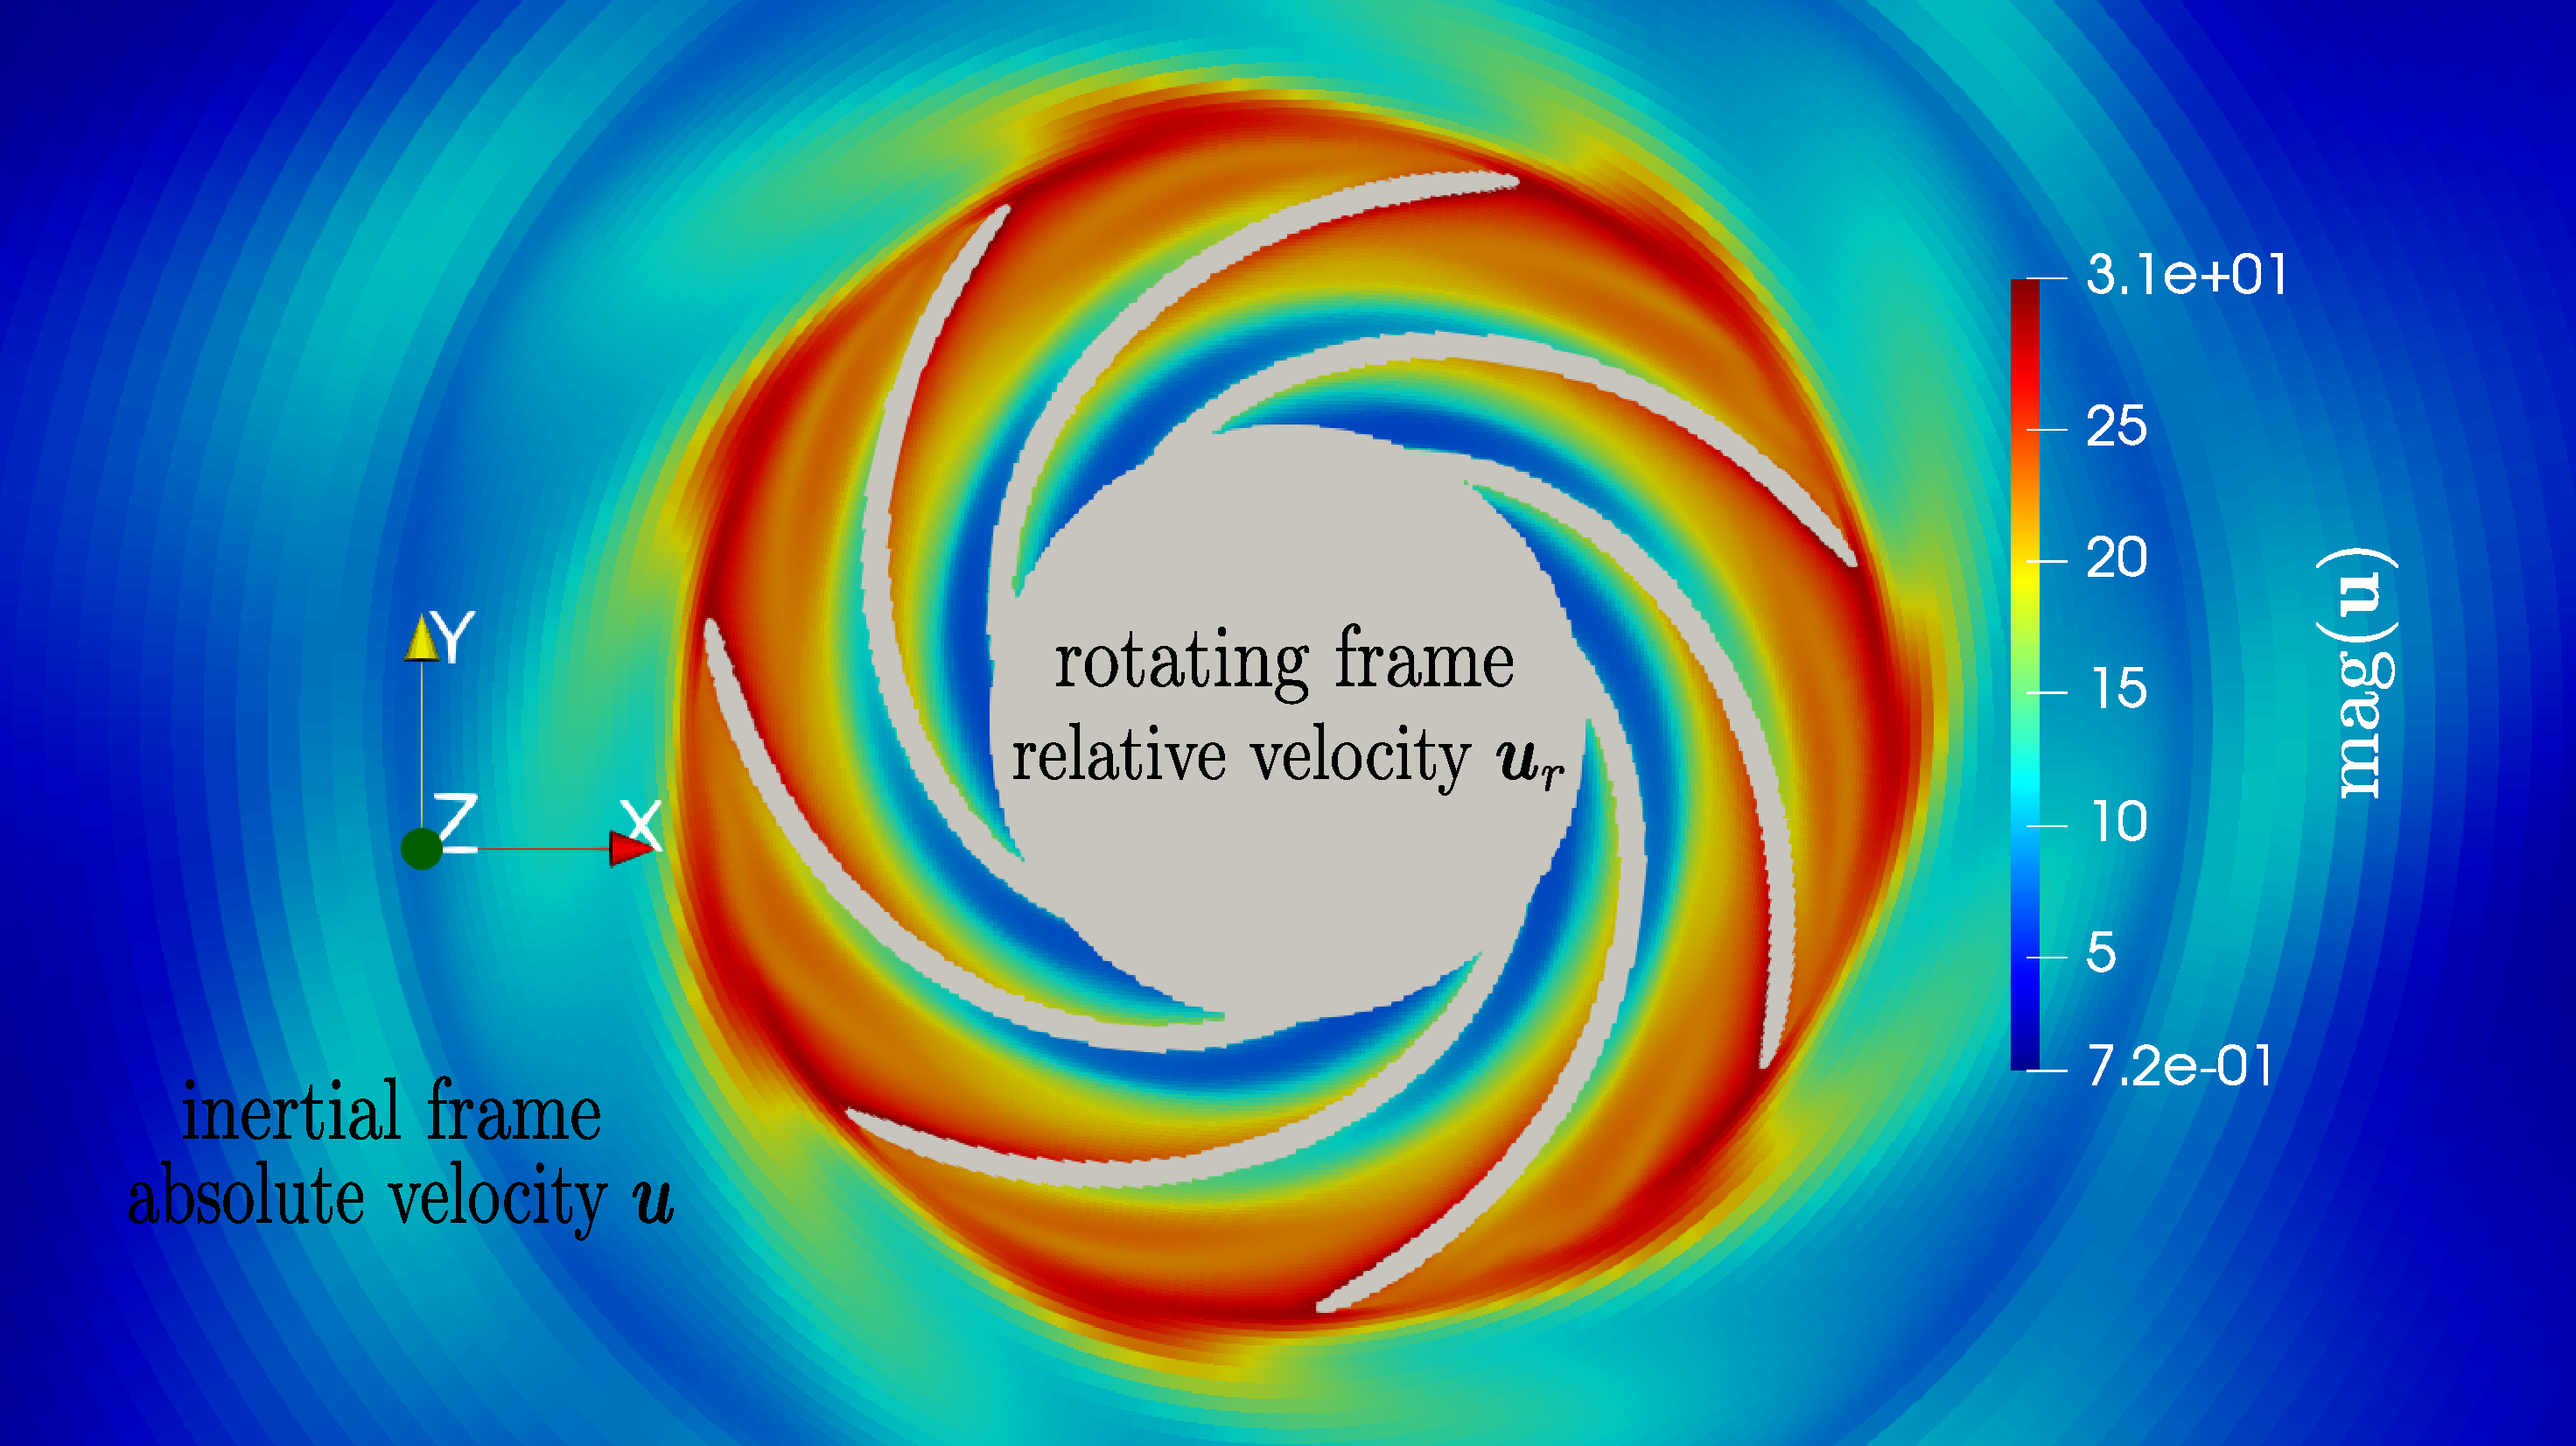
\includegraphics[width=0.8\textwidth]{../figures/velocity_profile.pdf}
            \end{column}
        \end{columns}
    \end{frame}

%\end{document}
\begin{frame}{Modélisation IBM}

    \begin{center}
        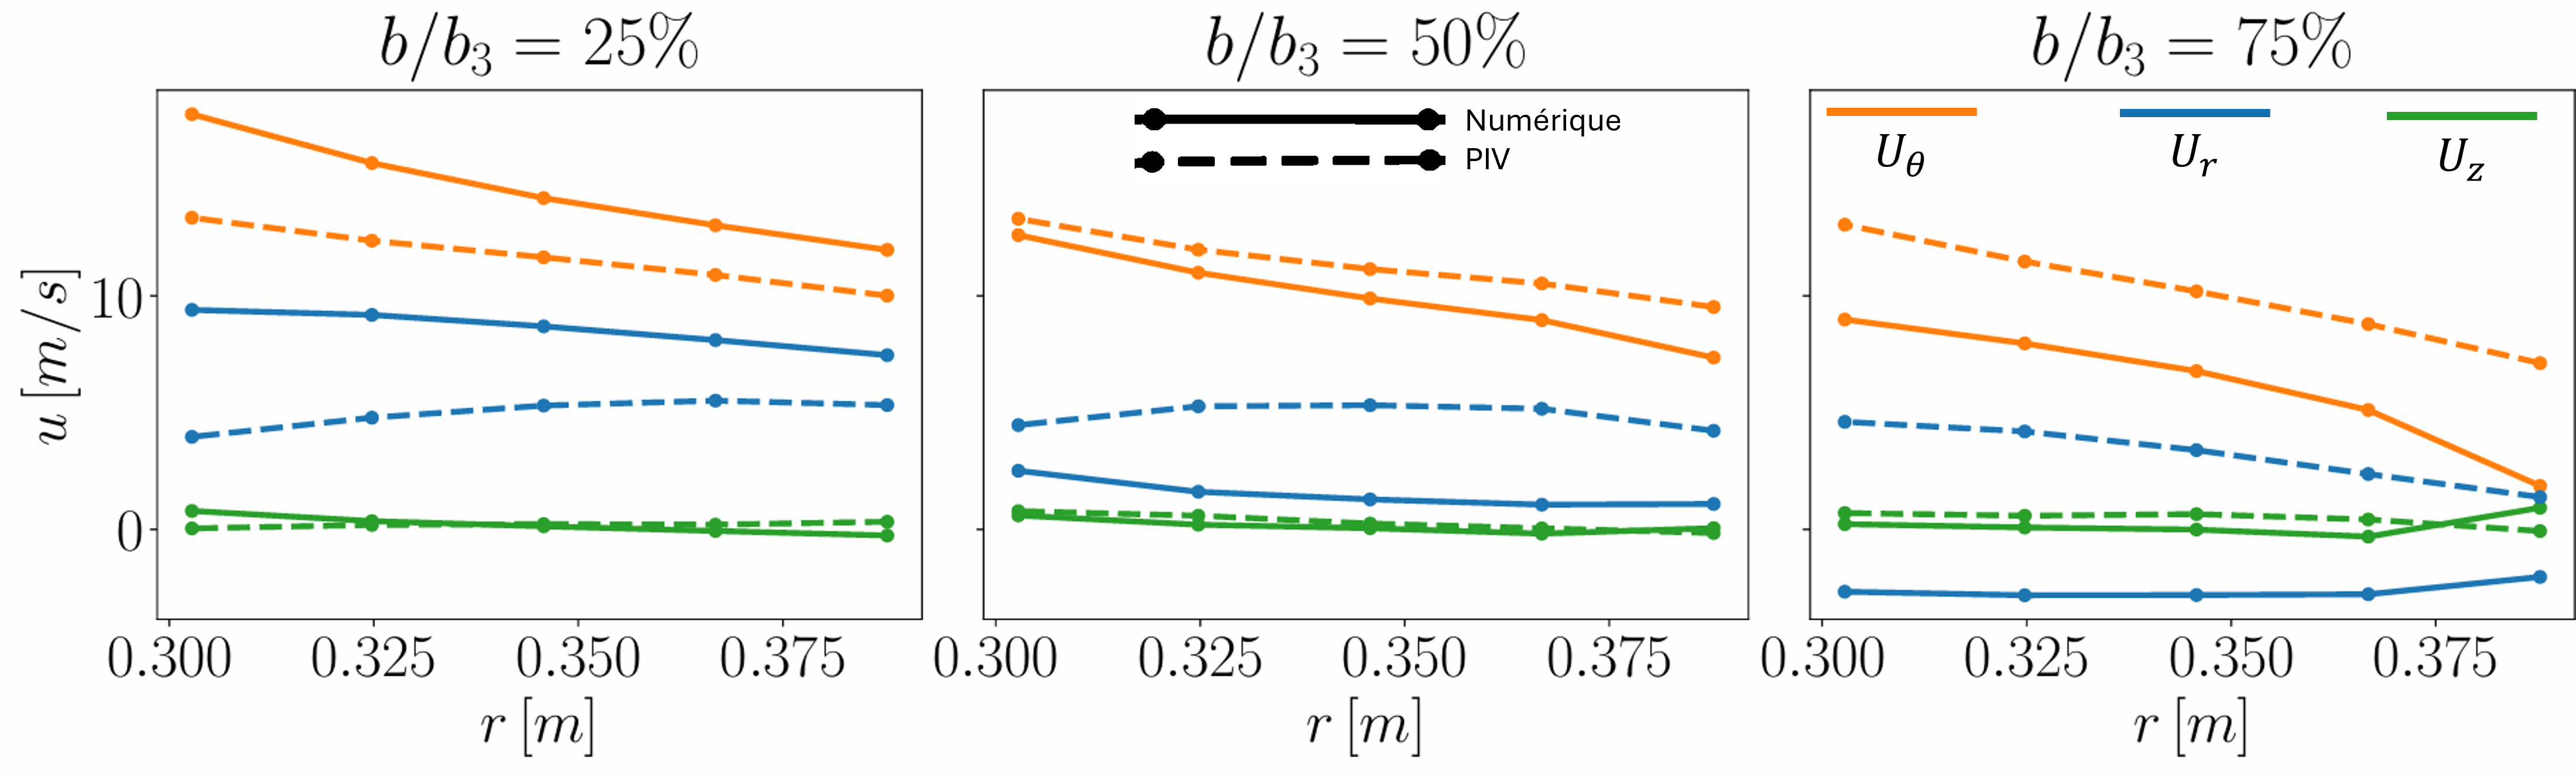
\includegraphics[scale=0.4]{../figures/numVSxpLegende.png}
        \scriptsize Comparaison entre les profils à l'intérieur du diffuseur pour la simulation numérique (lignes continues) et les données PIV (lignes pointillées). En particulier, (\protect\bluelinePython) représente la vitesse radiale $u_r$, (\protect\orangeline) montre la vitesse azimutale $u_\theta$, et (\protect\greenline) illustre la vitesse verticale $u_z$.
    \end{center}



    
\end{frame}



\begin{frame}{Modélisation IBM}

    \begin{columns}
        \begin{column}{0.5\linewidth}
            \begin{itemize}
                \item \texorpdfstring{\structure{\textbf{Performance du diffuseur expérimentale et numérique non identiques}}}{Performance du diffuseur expérimentale et numérique non identiques}

                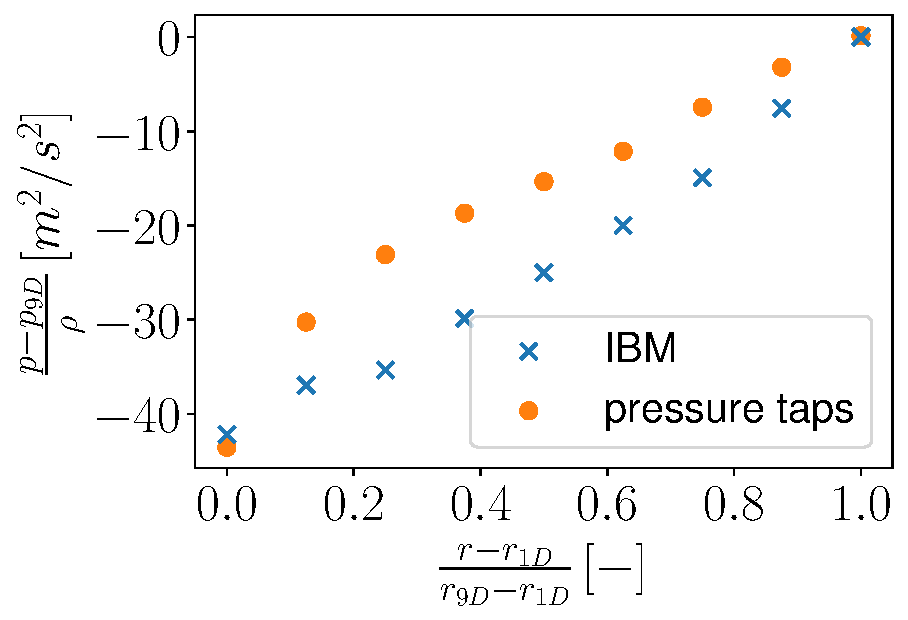
\includegraphics[scale=0.4]{../figures/diffuser_performance.pdf}

                %\item \structure{\textbf{Performance of the impeller}} still needs to be checked with different IBM coefficients $\eta$
            \end{itemize}
        \end{column}

        \only<1>{\begin{column}{0.5\linewidth}
            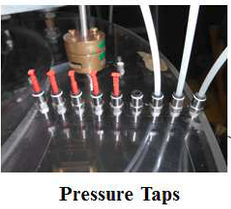
\includegraphics[scale=0.7]{../figures/pressure_taps.png}
        \end{column}}

        \only<2>{\begin{column}{0.5\linewidth}
            \centering
            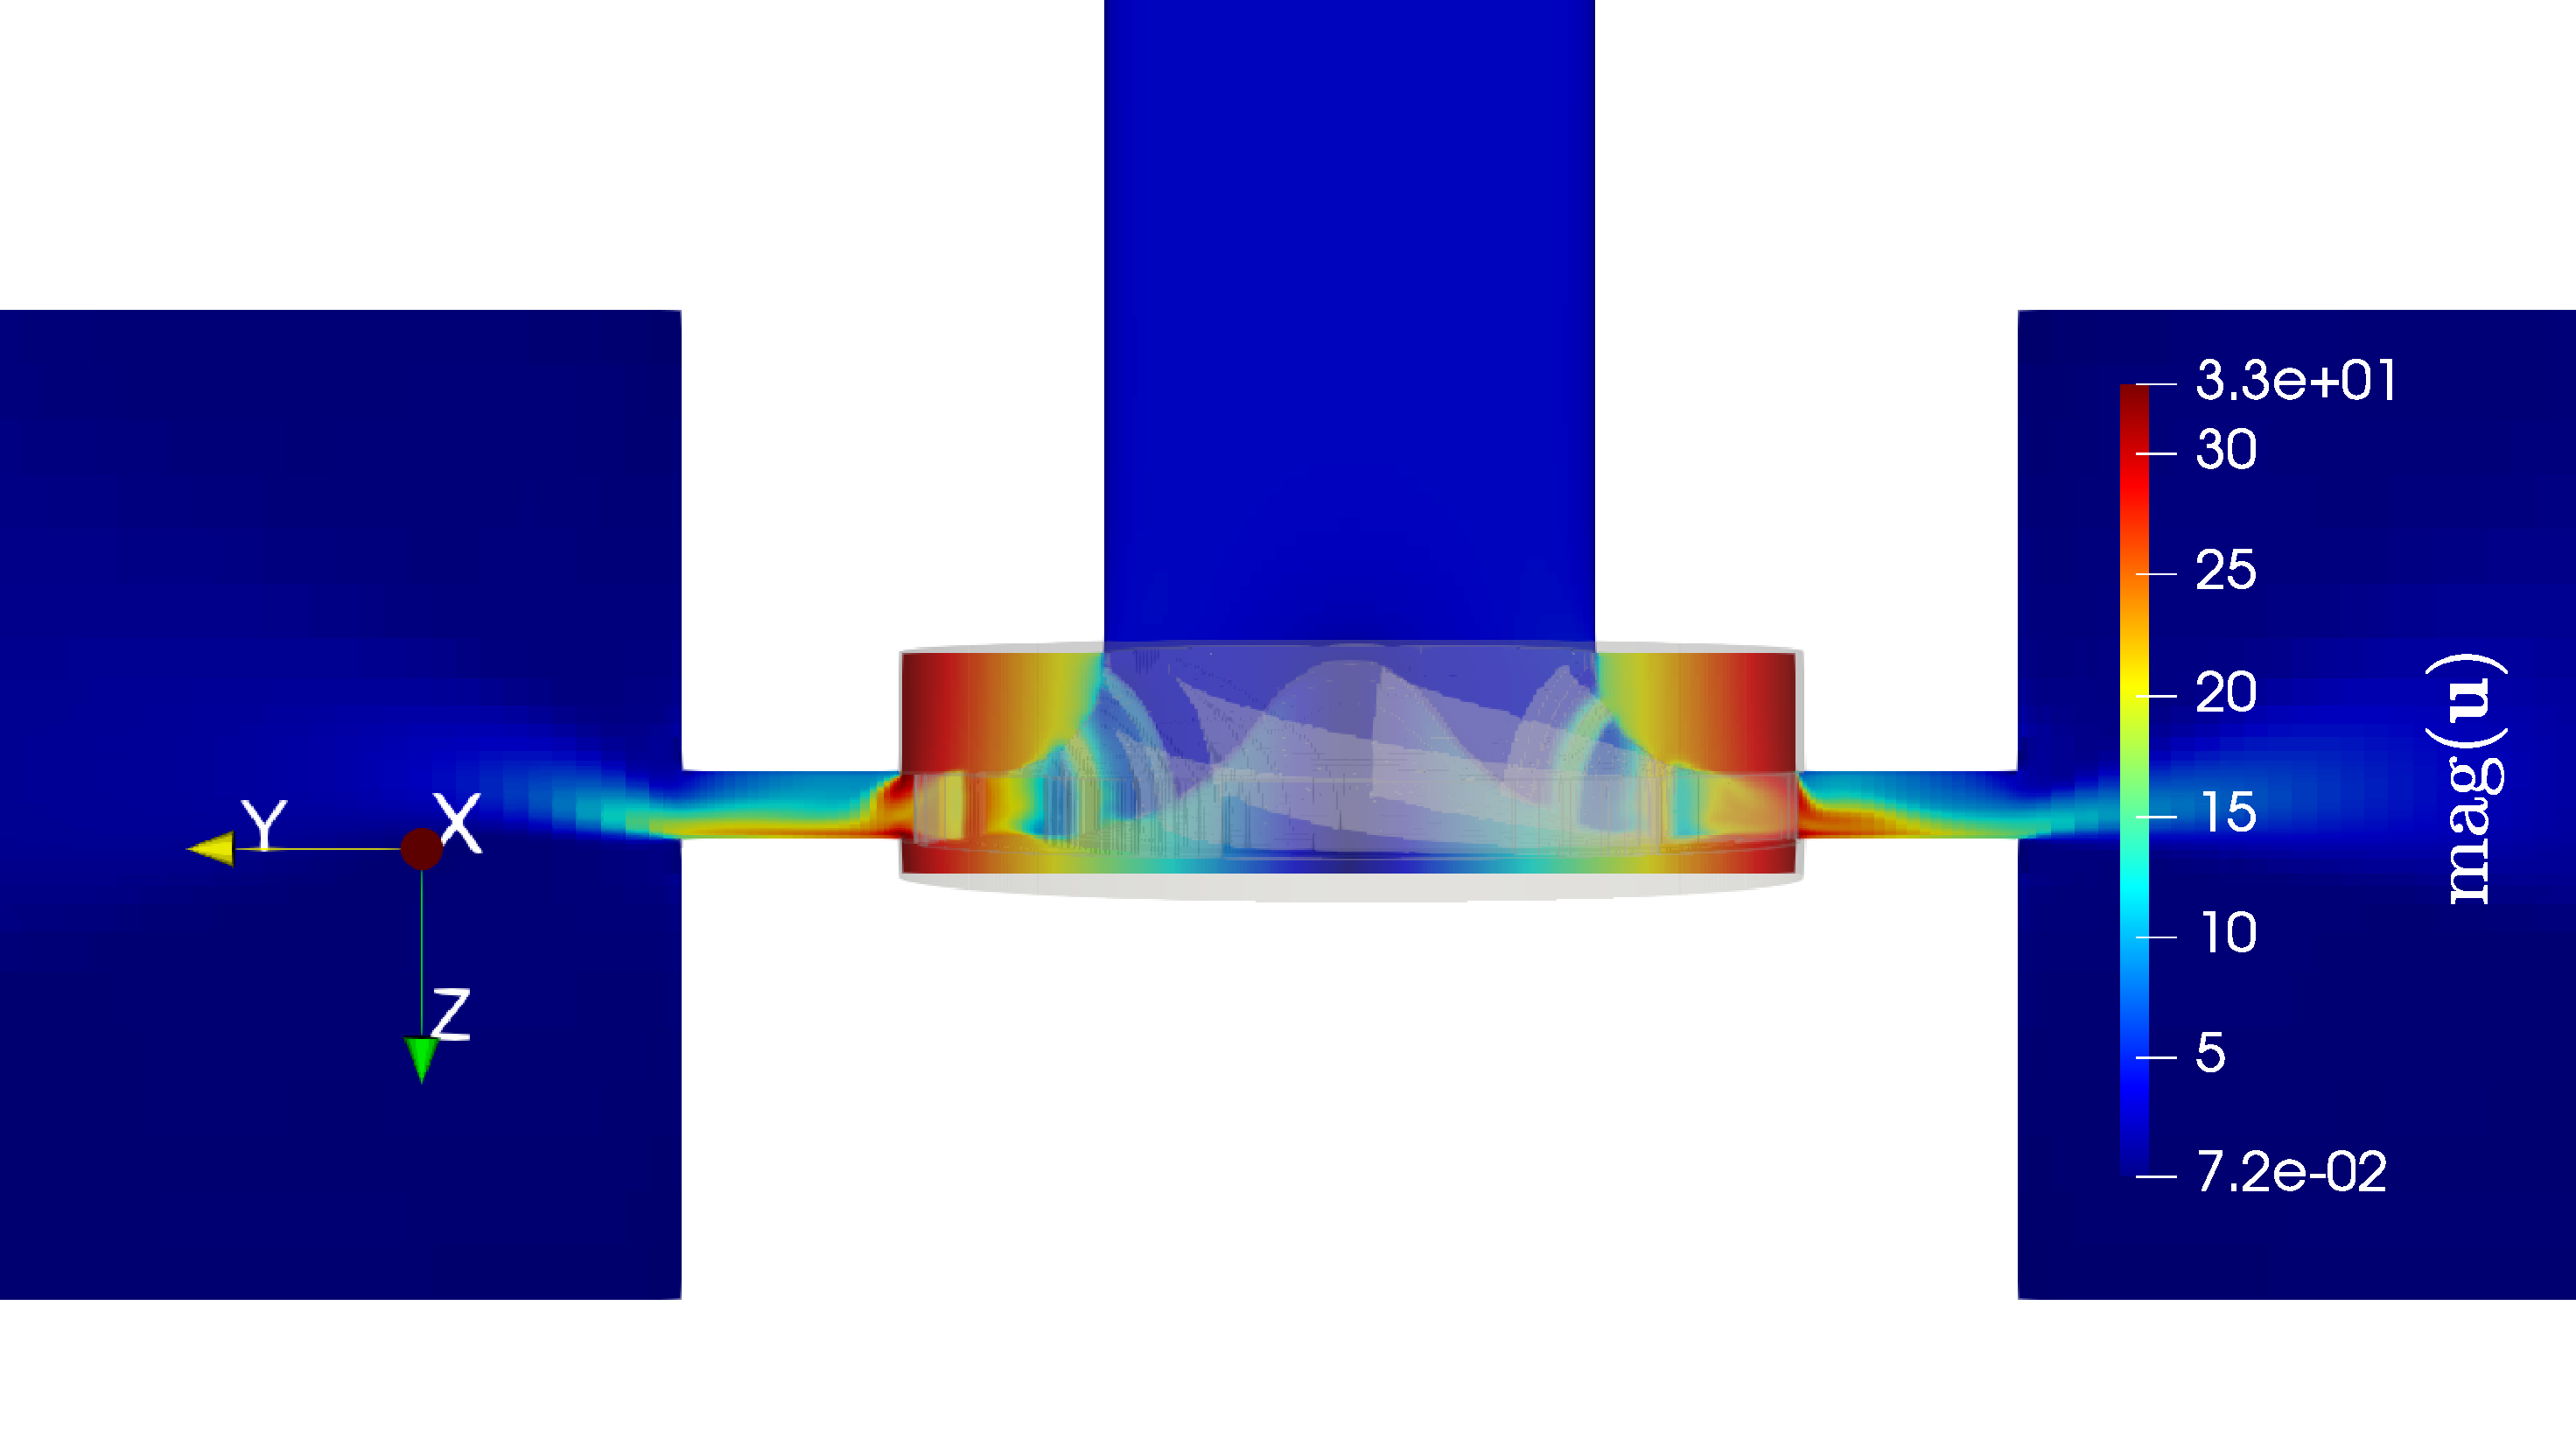
\includegraphics[width=0.9\textwidth]{../figures/velocity_verProfile.pdf}
            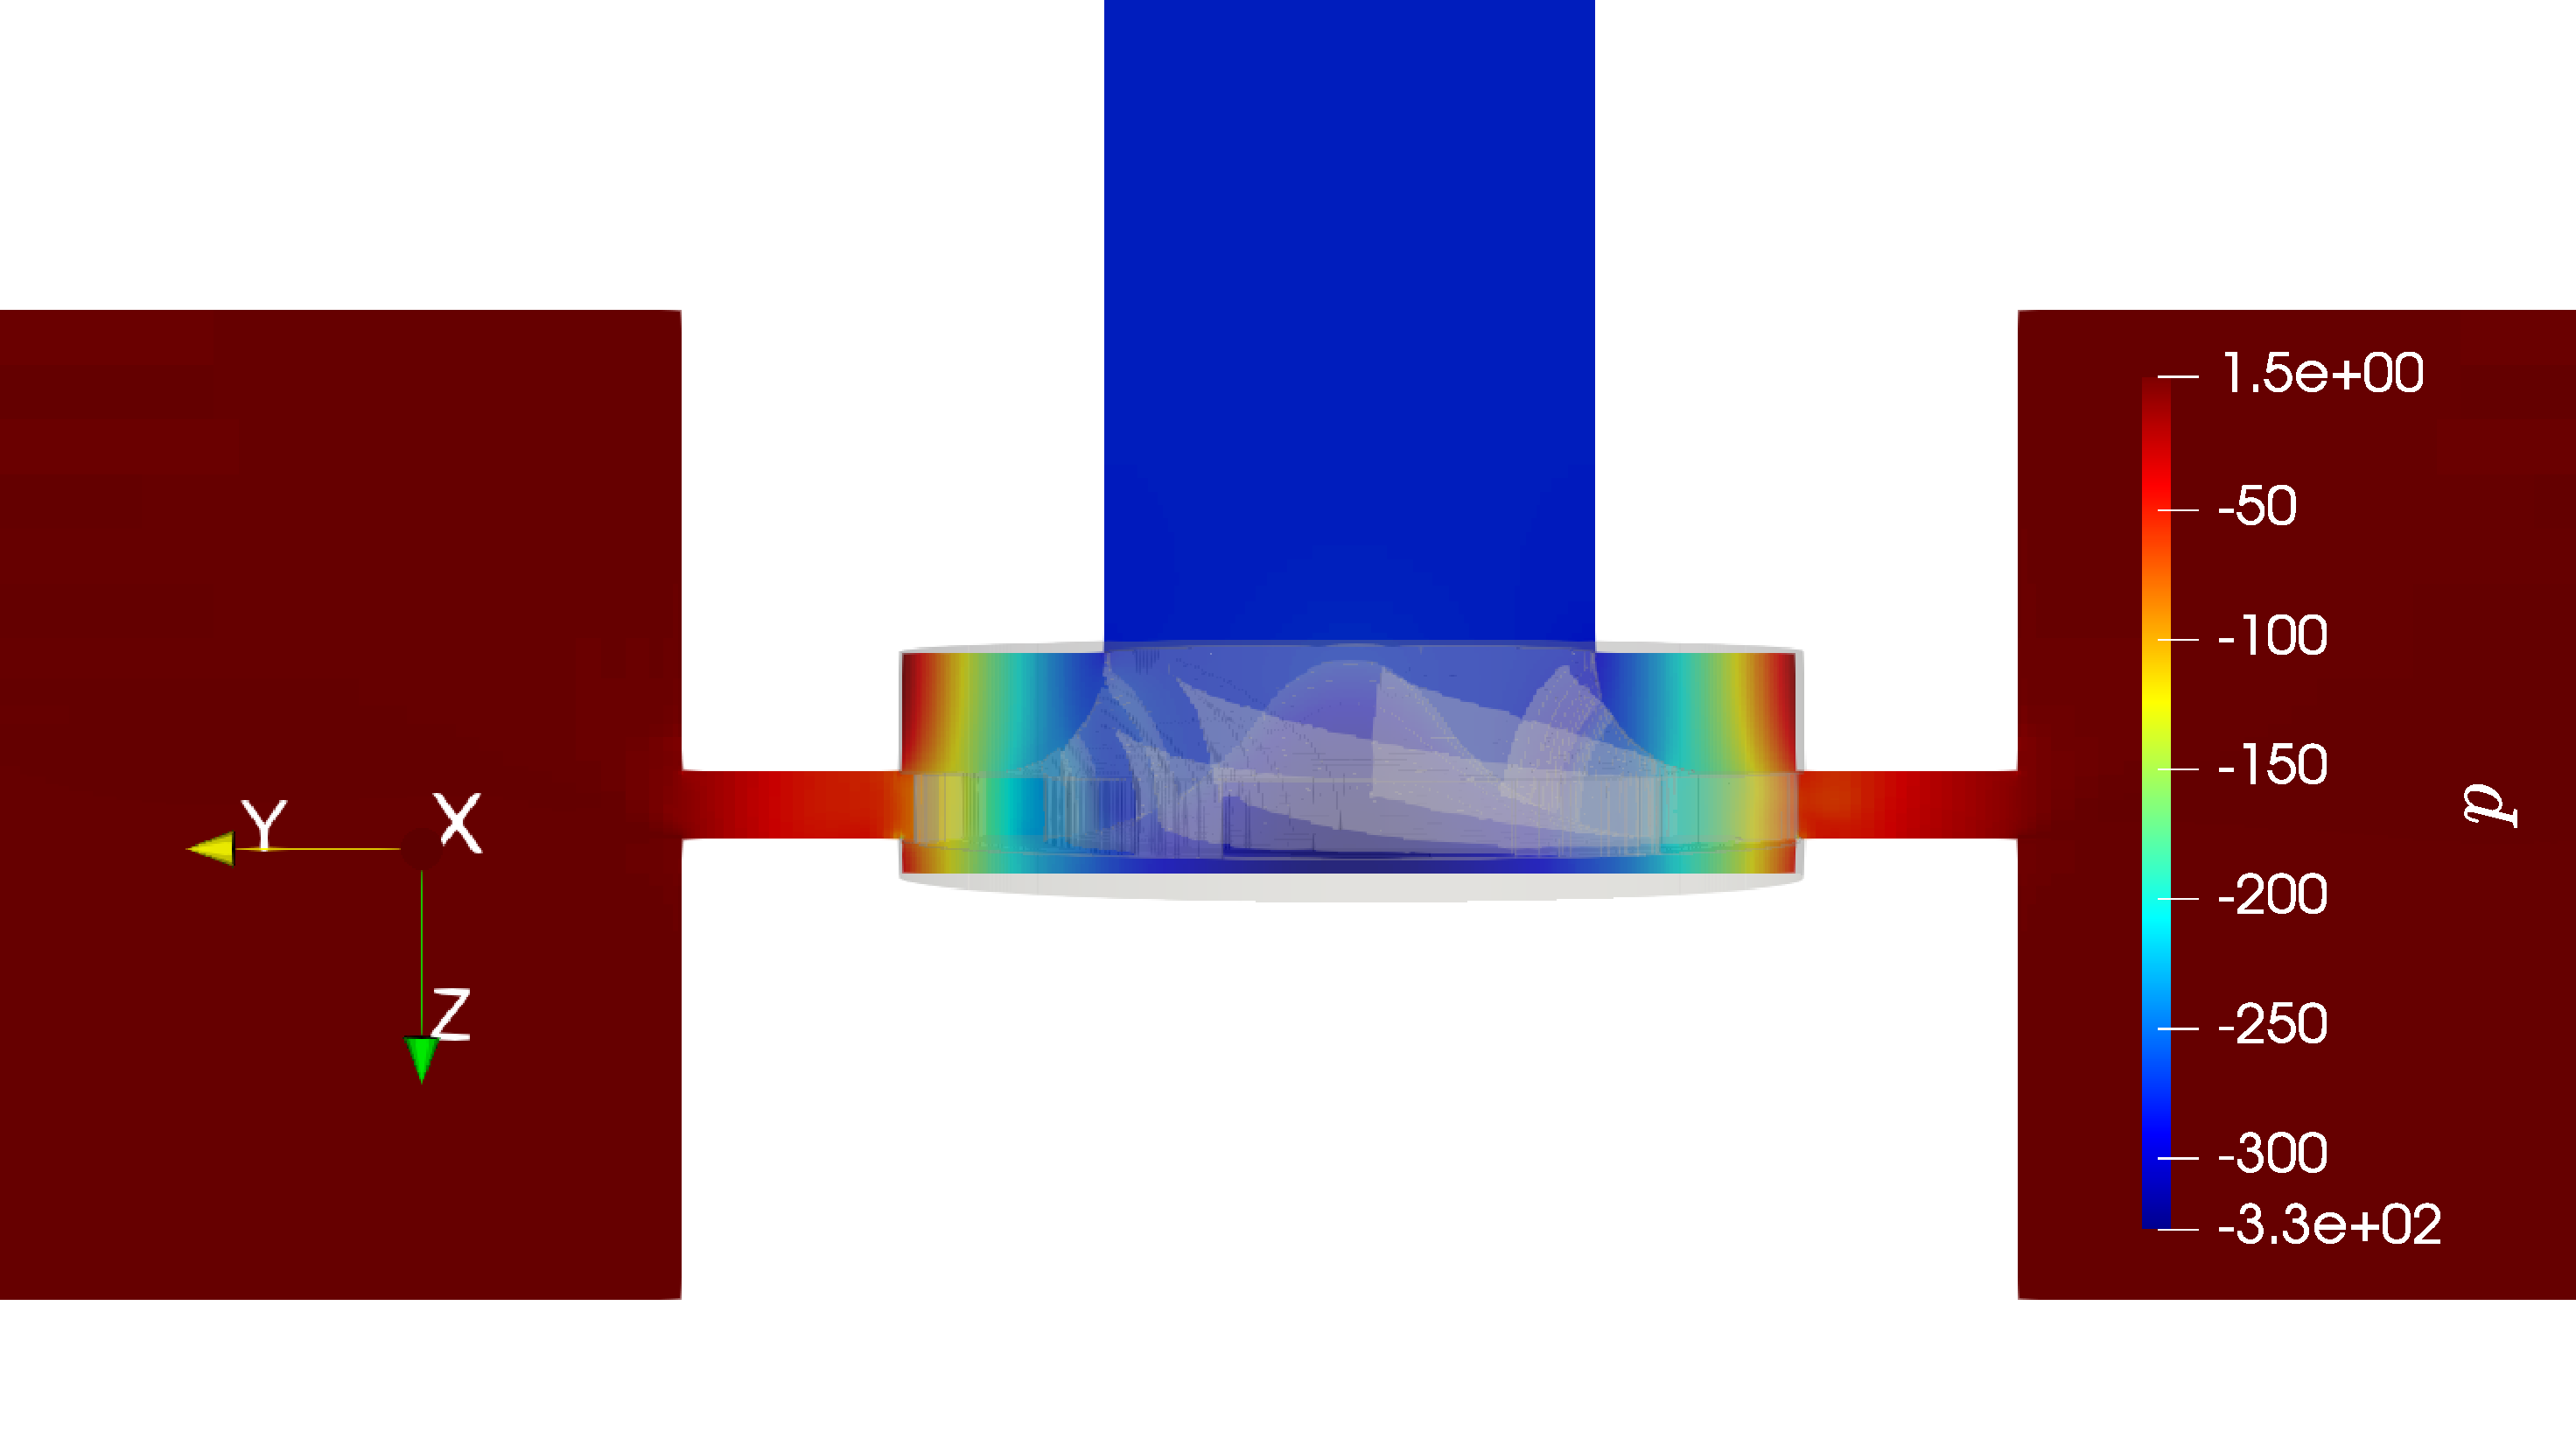
\includegraphics[width=0.9\textwidth]{../figures/pressure_verProfile.pdf}
        \end{column}}
        
    \end{columns}
    
\end{frame}


\begin{frame}{Limitations de la méthode IBM}

    \only<1>{%
        \centering
        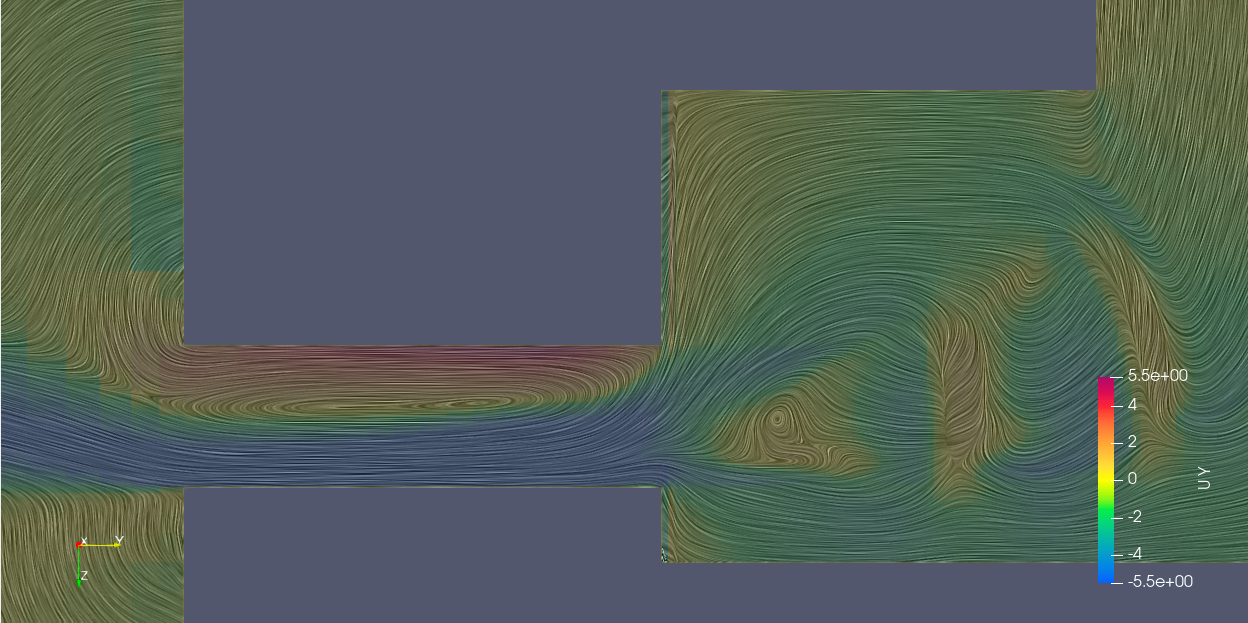
\includegraphics[width=0.8\linewidth]{../newFigures/LIC_Uy.png} \\
        \vspace{0.2cm}
        {\footnotesize Champ LIC (Line Integral Convolution) et $U_y$}
    }

    \only<2>{%
        \centering
        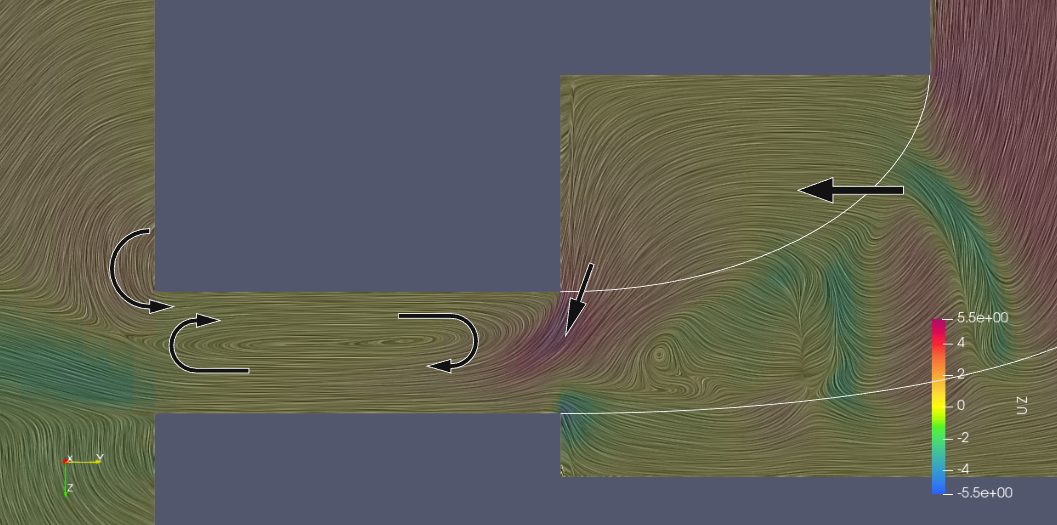
\includegraphics[width=0.8\linewidth]{../newFigures/LIC.png} \\
        \vspace{0.2cm}
        {\footnotesize Bulle de recirculation}
    }

\end{frame}

%\begin{frame}{DA avec l'EnKF - Premiers résultats}
    %\begin{figure}
        %\centering
        %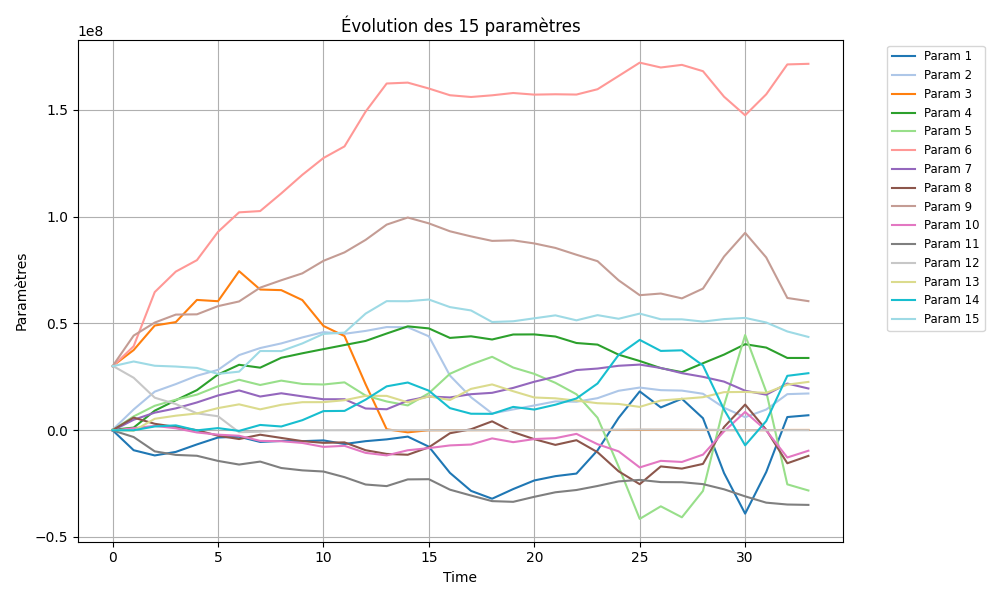
\includegraphics[width=0.6\linewidth]{../newFigures/UpdtC14_10params.png}
        %\caption{Enter Caption}
        %\label{fig:enter-label}
    %\end{figure}
%\end{frame}

%\begin{frame}{DA avec l'EnKF - Premiers résultats}
%\begin{figure}
    %\centering
    %\includegraphics[width=0.6\linewidth]{../newFigures/UpdtC14_NMRSE.png}
    %\caption{Enter Caption}
    %\label{fig:enter-label}
%\end{figure}
%\end{frame}

\begin{frame}{DA avec l'EnKF - Premiers paramètres}

    \begin{itemize}
        \item optimisation des 5 paramètres de forcage ($3\times$ vitesse, énergie turbulente et dissipation)
        \item pas d'optimisation d'état
        \item paramètres initiaux tous égaux à $3 \times 10^7$
        \item simulation RANS et données PIV moyennées temporellement
        \item fenêtre d'observation : 800 itérations
        \item 30 membres d'ensemble
        \item 45 observations ($Ur U_{\theta} Uz$) sur 5 points sur 3 plans
        \item bruit d'observation : 0,2 m/s, soit 1,5\% du max. d'observation sur la vitesse
        %\item pas d'inflation
    \end{itemize}

\end{frame}



\begin{comment}
    
\begin{frame}{\texorpdfstring{DA avec l'EnKF - Premiers résultats en stationaire}{DA avec l'EnKF - Premiers résultats en stationaire}}

    \begin{columns}
        
    \column{0.48\textwidth}
        \begin{figure}
            \centering
            
\includegraphics[width=0.6\linewidth]{new../figures/assymetrie.png}
            \caption{\texorpdfstring{Champs de vitesse absolue pour\\ Dx = 4e7 et Dy = 2e7}{Champs de vitesse absolue pour Dx = 4e7 et Dy = 2e7}}
            \label{fig:enter-label11}
        \end{figure}

    \column{0.48\textwidth}
        \begin{figure}
            \centering
            
\includegraphics[width=0.6\linewidth]{new../figures/coords.png}
            \caption{\texorpdfstring{Points d'observation de vitesse numérique avant moyenne azimutale}{Points d'observation de vitesse numerique avant moyenne azimutale}}
            \label{fig:enter-label12}
        \end{figure}


    \end{columns}

    Problème : mesure uniquement sur 1/7ème de la simulation numérique impliquant $Dx \neq Dy$.
    La NRMSE diminue car ces parmètres cassent la bulle de recirculation mais le résultat n'est pas physique.

\end{frame}
\end{comment}


\begin{frame}{DA avec l'EnKF - Premiers résultats}

    \begin{figure}
        \centering
        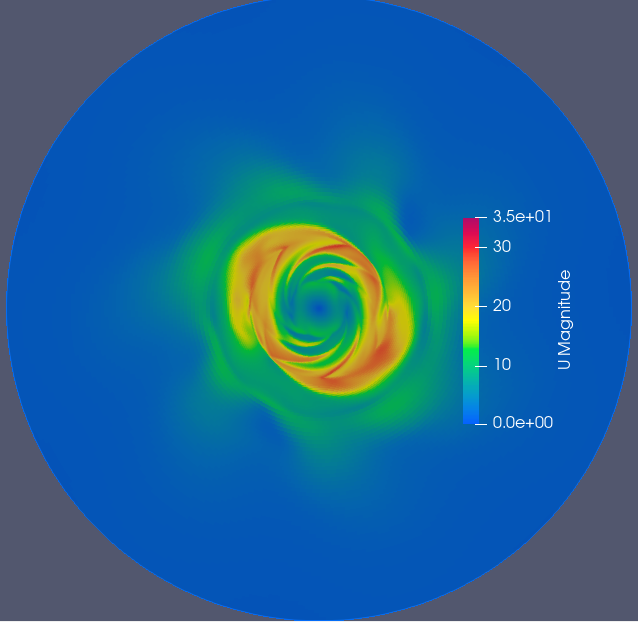
\includegraphics[width=0.4\linewidth]{../images/numericalPump/assymetrie.png}%{../newFigures/UpdtC14_10NMRSE.png} % Bulle de recirculation localement détruite
        \caption{Premier résultat de la DA :  $D = ({\boldsymbol{D_{u_x}}}, {\boldsymbol{D_{u_y}}}, {\boldsymbol{D_{u_z}}}, {D_\mathcal{K}}, {D_\omega}) = (4e7, 2e7, 4e7, 3e7, -3e7)$}
        \label{fig:1erResultat}
    \end{figure}

\end{frame}

%\begin{frame}{Limitations de la méthode IBM}
    %\begin{figure}
        %\centering
        %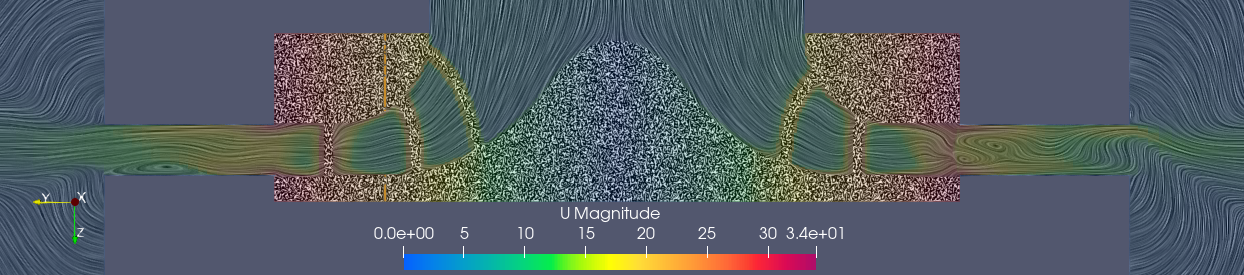
\includegraphics[width=0.9\linewidth]{../newFigures/pen0.png}
        %\caption{Enter Caption}
        %\label{fig:enter-label}
    %\end{figure}
%\end{frame}



\begin{frame}{DA avec l'EnKF - Nouvelles techniques}

    \begin{itemize}
        \item paramètres de forcage initiaux tous égaux à $3 \times 10^7$
        \item fenêtre d'observation : 800 itérations
        \item simulation RANS et données PIV moyennées temporellement
        \item pas d'optimisation d'état
        \item 30 membres d'ensemble
    \end{itemize}

    \setbeamercolor{item}{fg=red}

    \begin{itemize}
        \item Expansion radiale des paramètres de forcage $\boldsymbol{D}$ (permettant de décrire la courbe de l'aube) et optimisation des 12 paramètres de forcage $3\times (2\times$ vitesse, énergie turbulente et dissipation)
        \item 316 observations : ($Ur U_{\theta} Uz$) sur 7 sections (avec 5 points sur 3 plans) + observation globale de pression
        \item paramètres minorés à $0 + \left| \mathcal{N}(0, 1000) \right|$
        \item bruit d'observation : 0,2 m/s, soit 1,5\% du max. d'observation sur la vitesse et 5Pa soit 1,2\% du $\Delta P$ global sur la pression $\implies$ performance
    \end{itemize}

\end{frame}

\begin{frame}{DA avec l'EnKF - Nouvelles techniques}

    \setbeamercolor{item}{fg=red}
    \begin{itemize}
        \item Expansion radiale des paramètres $\boldsymbol{D_u}$ (permettant de décrire la courbe de l'aube) et optimisation des 12 paramètres de forcage $3\times (2\times$ vitesse, énergie turbulente et dissipation)
    \end{itemize}

    \begin{columns}[c]

        \column{0.48\textwidth}
            \begin{figure}
                \centering
                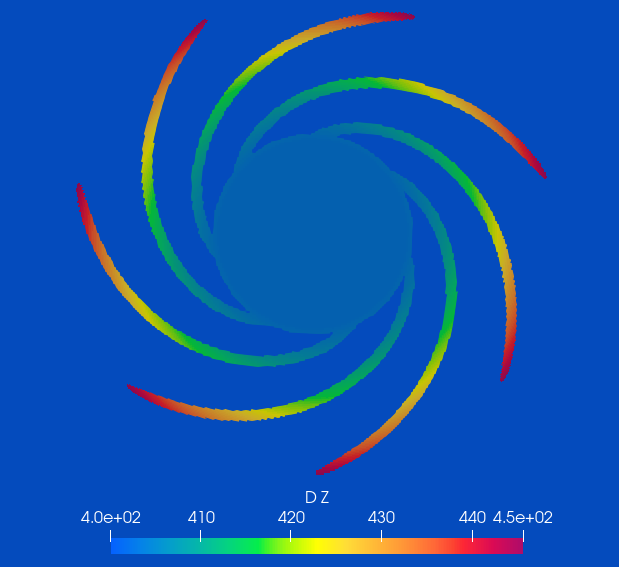
\includegraphics[width=0.55\linewidth]{../newFigures/radial_exp.png}
                \caption{Expansion radiale}
                \label{fig:enter-label42}
            \end{figure}

        \column{0.48\textwidth}
                \[
                \text{coeff} = 
                \begin{cases}
                a \cdot r_{\text{min}}^2 + b \cdot r_{\text{min}} + c & \text{si } r < r_{\text{min}} \\
                a \cdot r^2 + b \cdot r + c & \text{sinon}
                \end{cases}
                \]       
    \end{columns}
    

\end{frame}

\begin{frame}{DA avec l'EnKF - Nouvelles techniques}

    \begin{columns}[c]

        \column{0.48\textwidth}
        \setbeamercolor{item}{fg=red}
        \vspace{-2cm}
        \begin{itemize}
            \item 106 observations : ($Ur U_{\theta} Uz$) sur 7 sections (avec 5 points sur 3 plans) + observation globale de pression
        \end{itemize}

        \phantom{-}

        Évite un résultat de l'EnKF où les paramètres de forcage de l'IBM cassent la périodicité.

        \column{0.48\textwidth}
            \begin{figure}
                \centering
                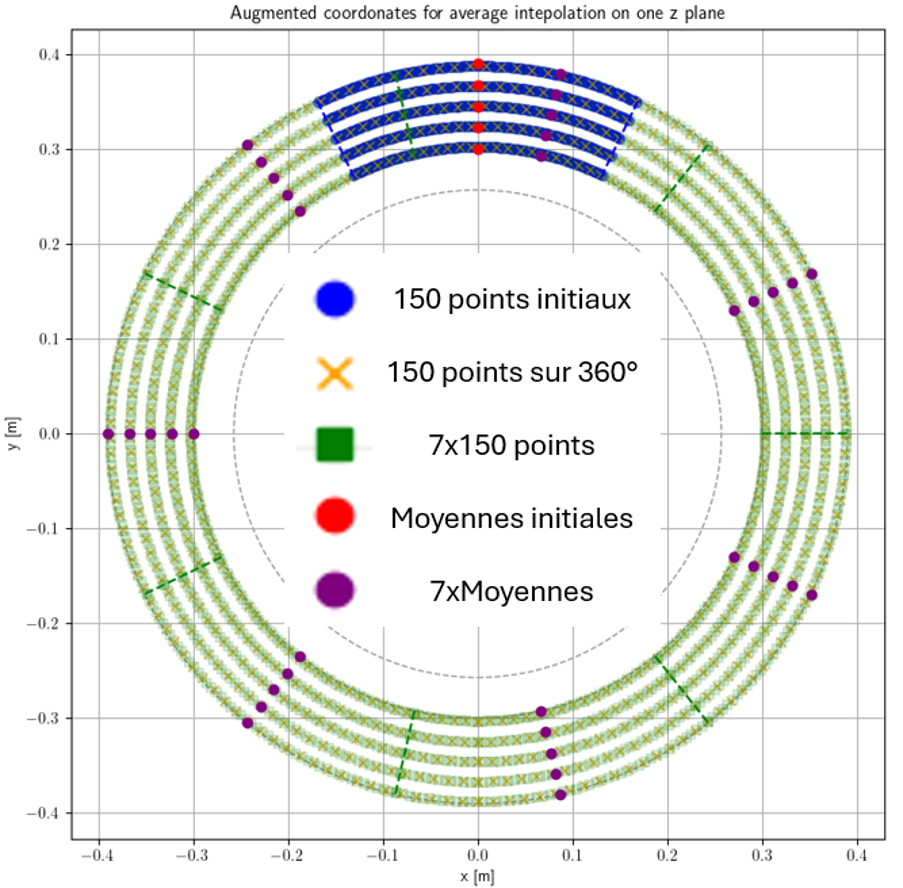
\includegraphics[width=0.85\linewidth]{../newFigures/coordsBis.png}
                %\caption{Points d'observation de vitesse numérique avant moyenne azimutale}
                \label{fig:enter-label5}
            \end{figure}
            
    \end{columns}

\end{frame}


\begin{frame}
    \begin{figure}
        \centering
        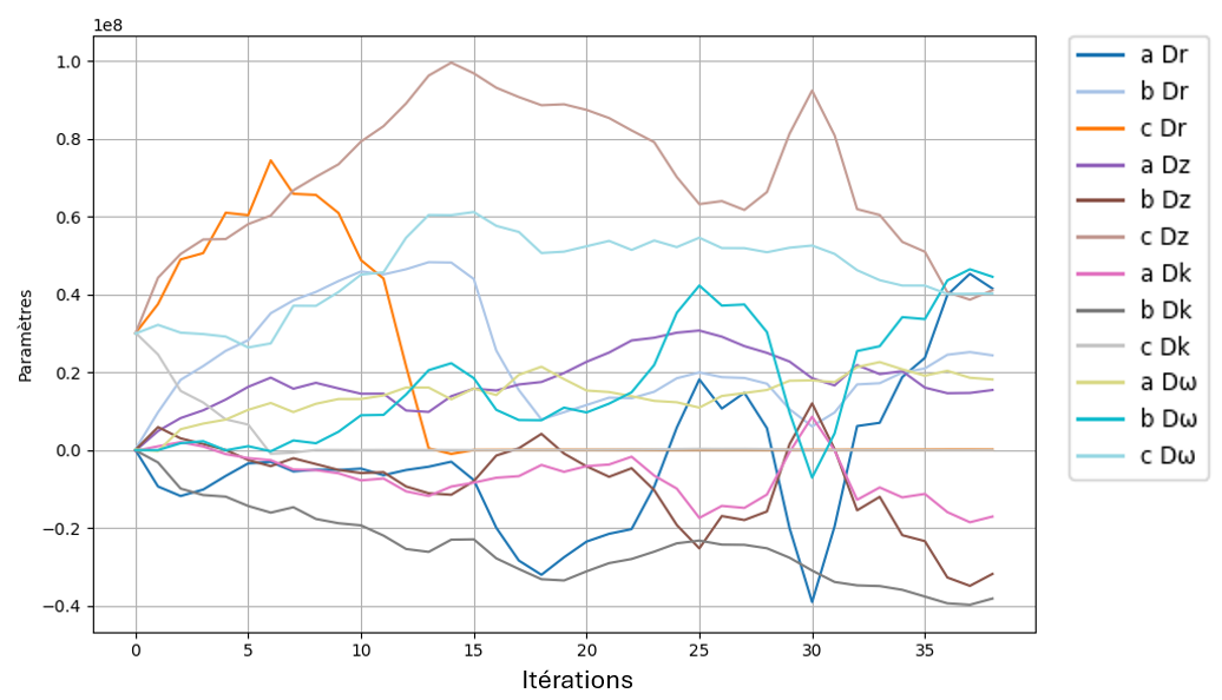
\includegraphics[width=0.7\linewidth]{../images/graph/UpdtC14_12paramsNew.png} % 
        \caption{Evolution des 12 paramètres de l'IBM au cours des itérations de l'EnKF}
        \label{fig:NRMSE1}
    \end{figure}
\end{frame}

\begin{frame}
    \begin{figure}
        \centering
        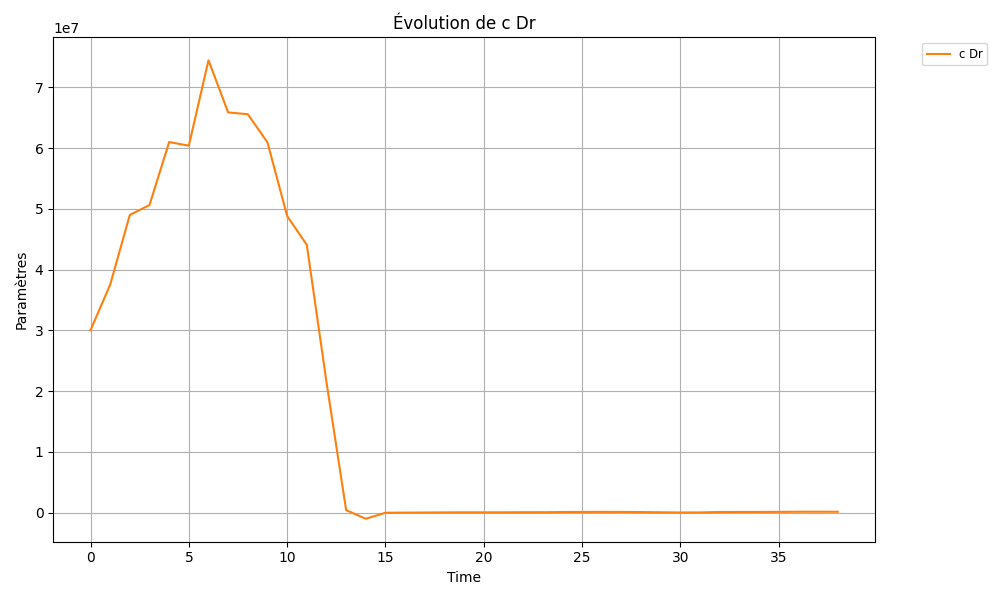
\includegraphics[width=0.7\linewidth]{../images/graph/cdr.png} % 
        \caption{Evolution du coefficient c Dr de l'IBM au cours des itérations de l'EnKF}
        \label{fig:NRMSE2}
    \end{figure}
\end{frame}


\begin{frame}{DA avec l'EnKF - Nouveaux résultats}

    \begin{figure}
        \centering
        % La première image apparaît sur la première étape (<1>)
        \only<1>{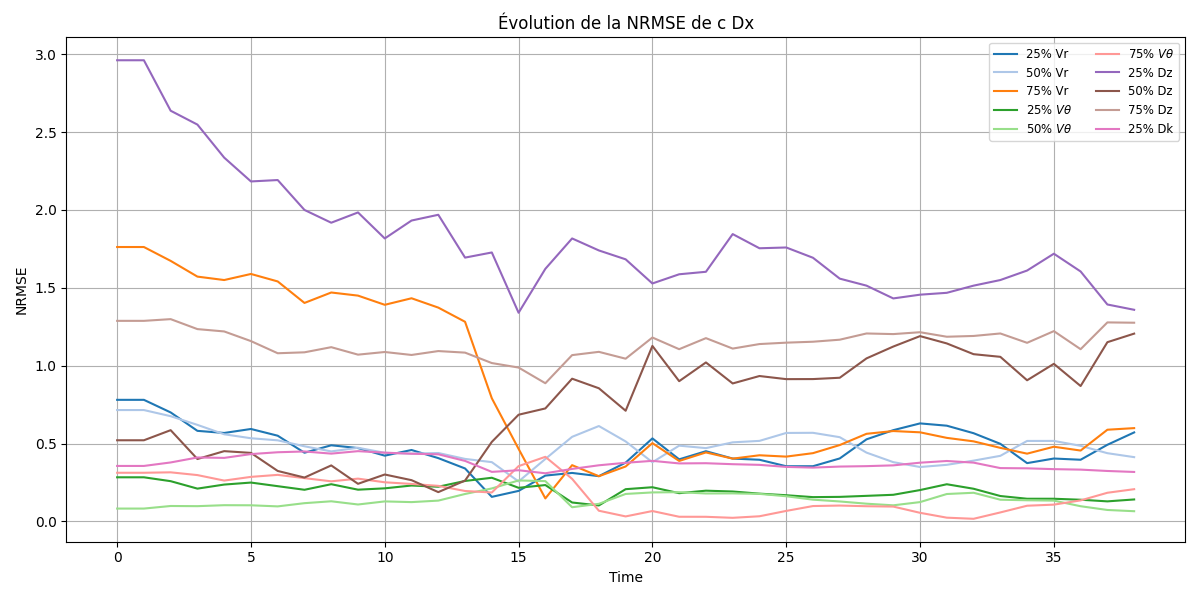
\includegraphics[width=0.65\linewidth]{../images/graph/NRMSE10.png}} %/newFigures/UpdtC14_10NMRSE.png}}
        % La deuxième image apparaît sur la deuxième étape (<2>)
        \only<2>{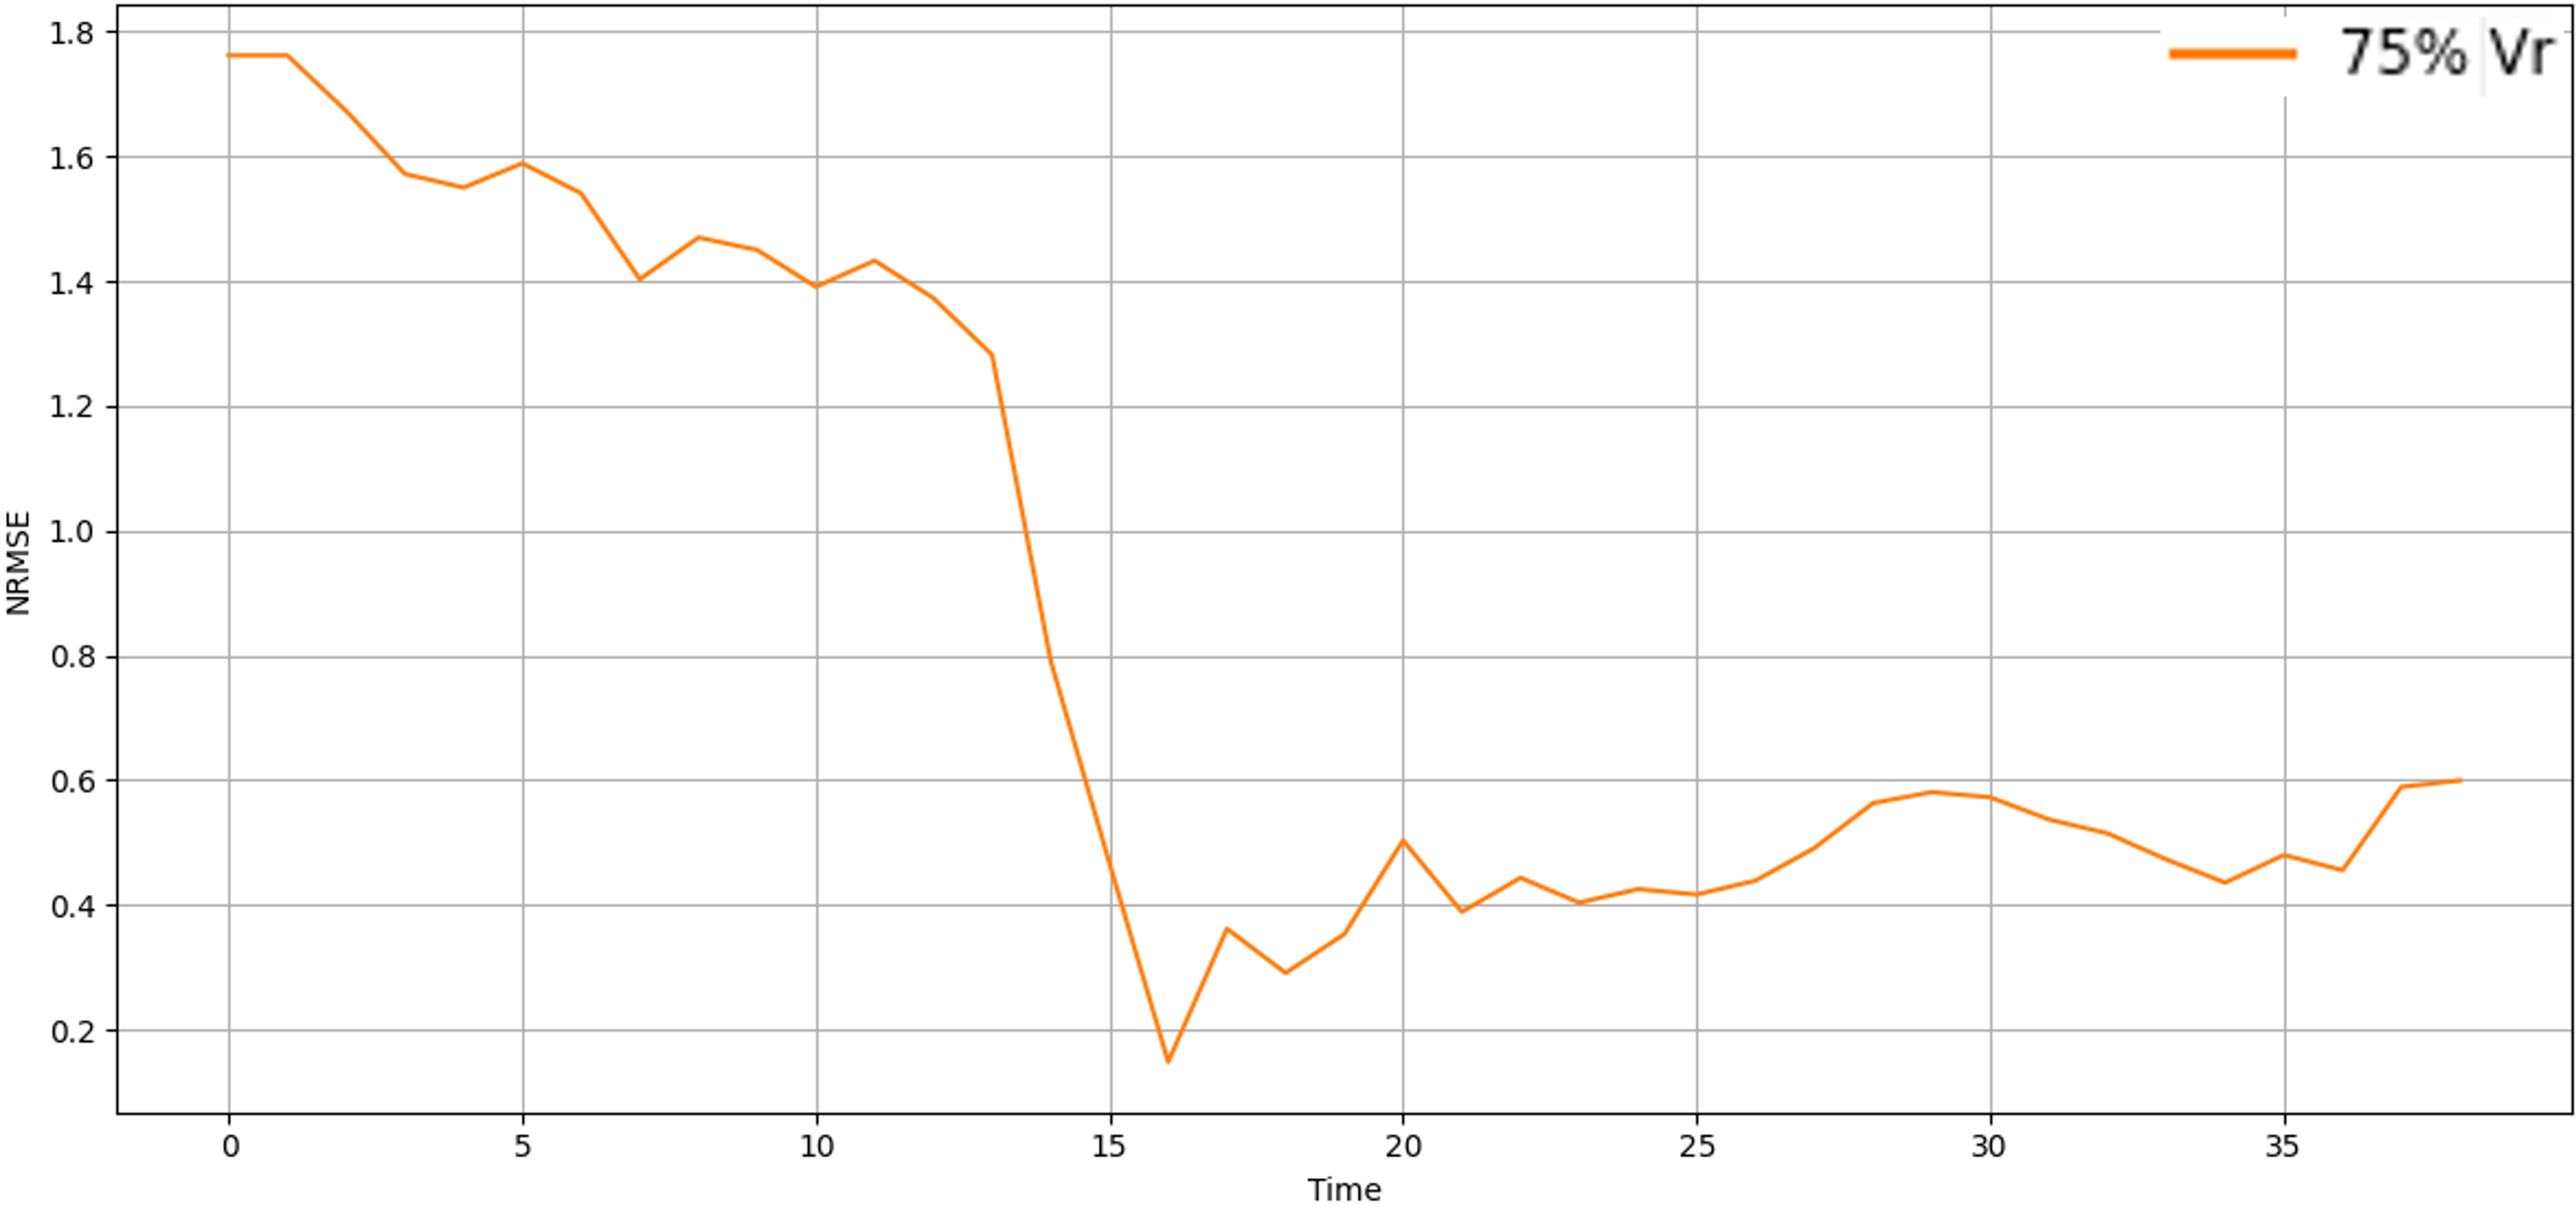
\includegraphics[width=0.65\linewidth]{../images/graph/cdxbis.png}}
        \caption{Bulle de recirculation détruite mais résultat non physique}
        \label{fig:10NRMSE} % Attention : il est préférable d'avoir des labels uniques si possible
    \end{figure}

    Diminution moyenne de l'erreur (Normalized Root Mean Square Error) de quelques pourcents, avec des variations de paramètres de forcage dépendantes des conditions initiales.

\end{frame}







\begin{frame}
    \begin{figure}
        \centering
        \includegraphics[width=0.7\linewidth]{../images/UpdtC14_NMRSE.png} % 
        \caption{Evolution de l'écart entre la simulation et l'expériemental au cours des itérations de l'EnKF}
        \label{fig:NRMSE}
    \end{figure}
\end{frame}

\begin{comment}
    \begin{frame}{DA avec l'EnKF - Nouveaux résultats}
        \begin{columns}[c]
            \column{0.48\textwidth}
                \begin{figure}
                    \centering
                    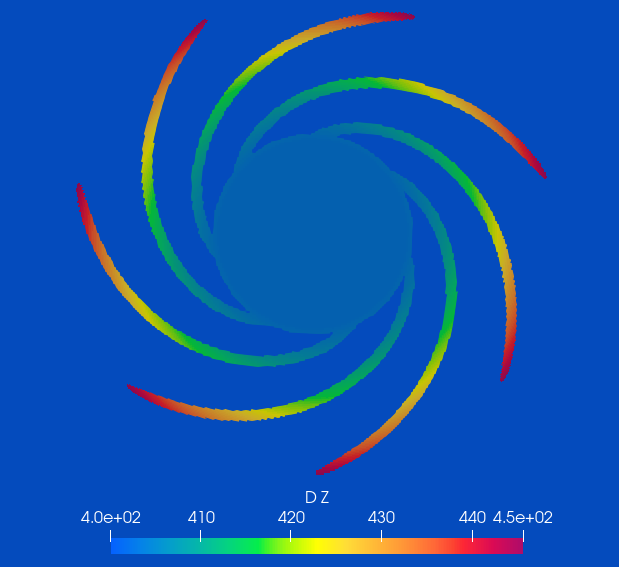
\includegraphics[width=0.7\linewidth]{../newFigures/radial_exp.png}
                    \caption{Expansion radiale}
                    \label{fig:expRad}
                \end{figure}
            \column{0.48\textwidth}
                \begin{figure}
                    \centering
                    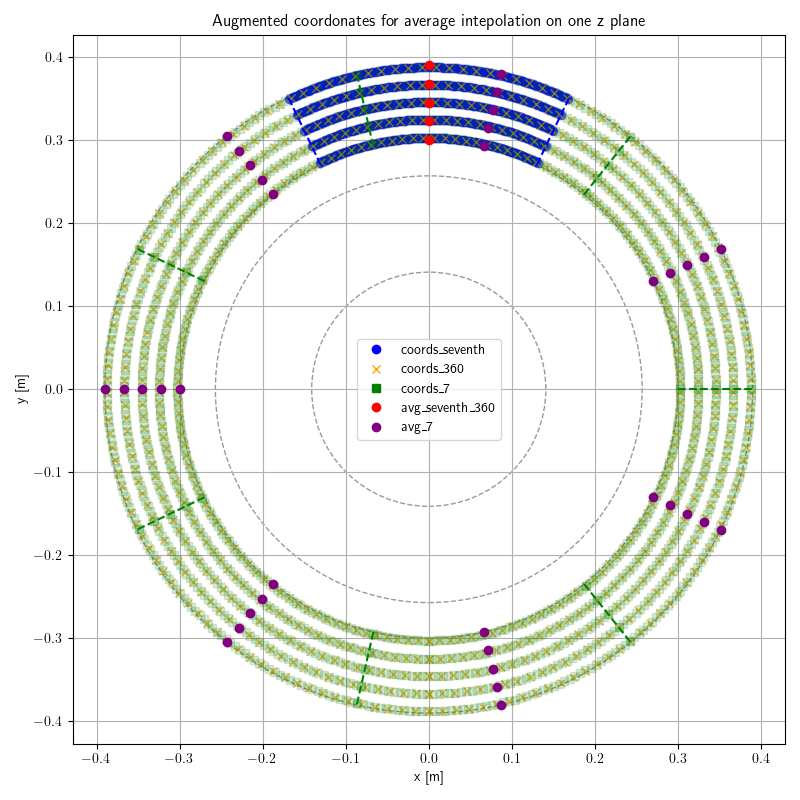
\includegraphics[width=0.7\linewidth]{../newFigures/coords.png}
                    \caption{Points d'observation de vitesse numérique avant moyenne azimutale}
                    \label{fig:enter-label7}
                \end{figure}
        \end{columns}
    \end{frame}
\end{comment}


%%%%%%%%%%%%%%%%%%%%%%%%%%%%%%%%%%%%%%%%%%%%%%%%%%%%%%%%%%%%%%%%%%%%%%%%%%%%%%%%%%%%%%%%%%%%
\section{Conclusion et perspectives}
%%%%%%%%%%%%%%%%%%%%%%%%%%%%%%%%%%%%%%%%%%%%%%%%%%%%%%%%%%%%%%%%%%%%%%%%%%%%%%%%%%%%%%%%%%%%

    \begin{frame}{Conclusion}
        \begin{itemize}
            \item<+-> {\color{green!60!black}\ding{51}}~ Mise en avant des limitations de la méthode aux frontières immergées (IBM)
            \item<+-> {\color{green!60!black}\ding{51}}~ Préparation des données expérimentales (PIV)
            \item<+-> {\color{green!60!black}\ding{51}}~ Intégration d'algorithme d'assimilation de données
            \item<+-> {\color{orange}\textbullet}~ Optimisation des paramètres de la méthode IBM
            % \item<+-> {\color{green!60!black}\ding{51}}~ Valider les résultats obtenus par rapport aux données expérimentales
        \end{itemize}
    \end{frame}



    \begin{frame}{Perspectives}
        \begin{columns}[c]

            \column{0.48\textwidth}
                \begin{itemize}
                    \item Passage de la simulation en instationnaire permettant notamment de ne plus utiliser l'approche MRF
                    \item Imposition d'une condition de paroi sur le « carénage » de la pompe avec un maillage body-fitted
                    \item Utilisation d'une méthode IBM plus sophistiquée
                    \end{itemize}
            
            \column{0.48\textwidth}
                \begin{figure}
                    \centering
                    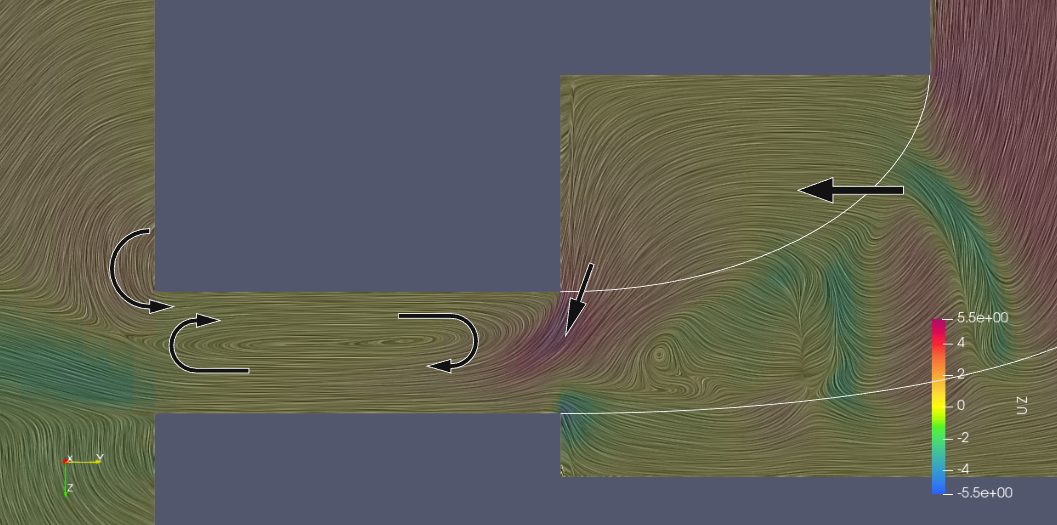
\includegraphics[width=1\linewidth]{../newFigures/LIC.png}
                    \caption{Bulle de recirculation}
                    \label{fig:enter-label8}
                \end{figure}
                
        \end{columns}

    \end{frame}

    \begin{frame}{Perspective : simulation instationnaire}

        \begin{columns}[c]

            \column{0.48\textwidth}
                \centering
                \animategraphics[loop, autoplay, width=0.9\linewidth]{2}{../images/rotating/}{1}{5}
                \scriptsize Rotation de la partie pénalisée, parallélisé sur 4 cœurs
            
            \column{0.48\textwidth}
                \centering
                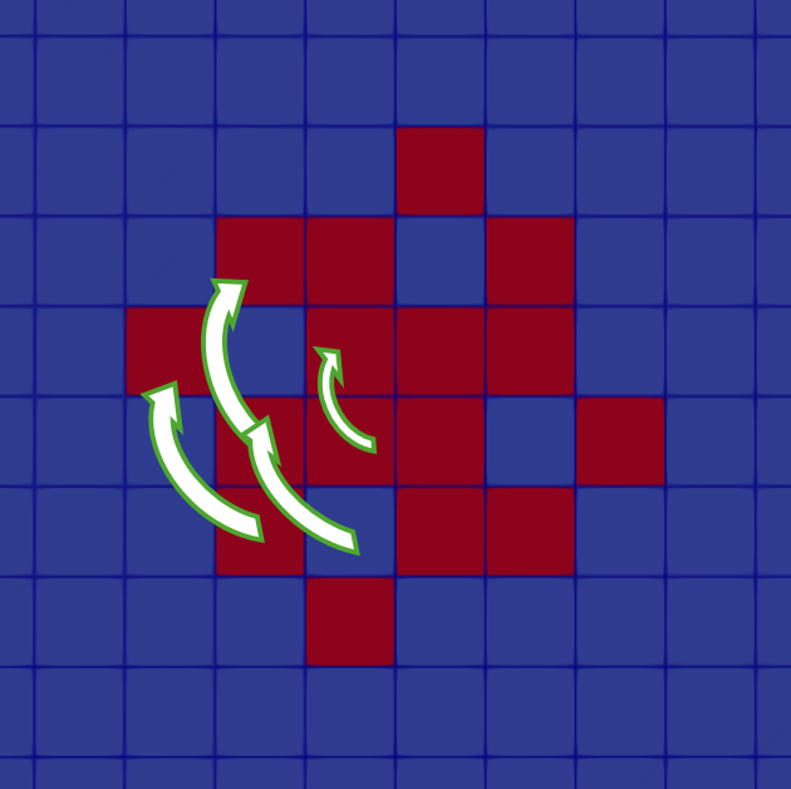
\includegraphics[width=0.9\linewidth]{../images/rotating/3bisbis.png}
                \scriptsize Déplacement de la partie pénalisée

        \end{columns}

    \end{frame}

    
    \begin{frame}{A venir}
        \begin{columns}
            \begin{column}{0.55\textwidth}
                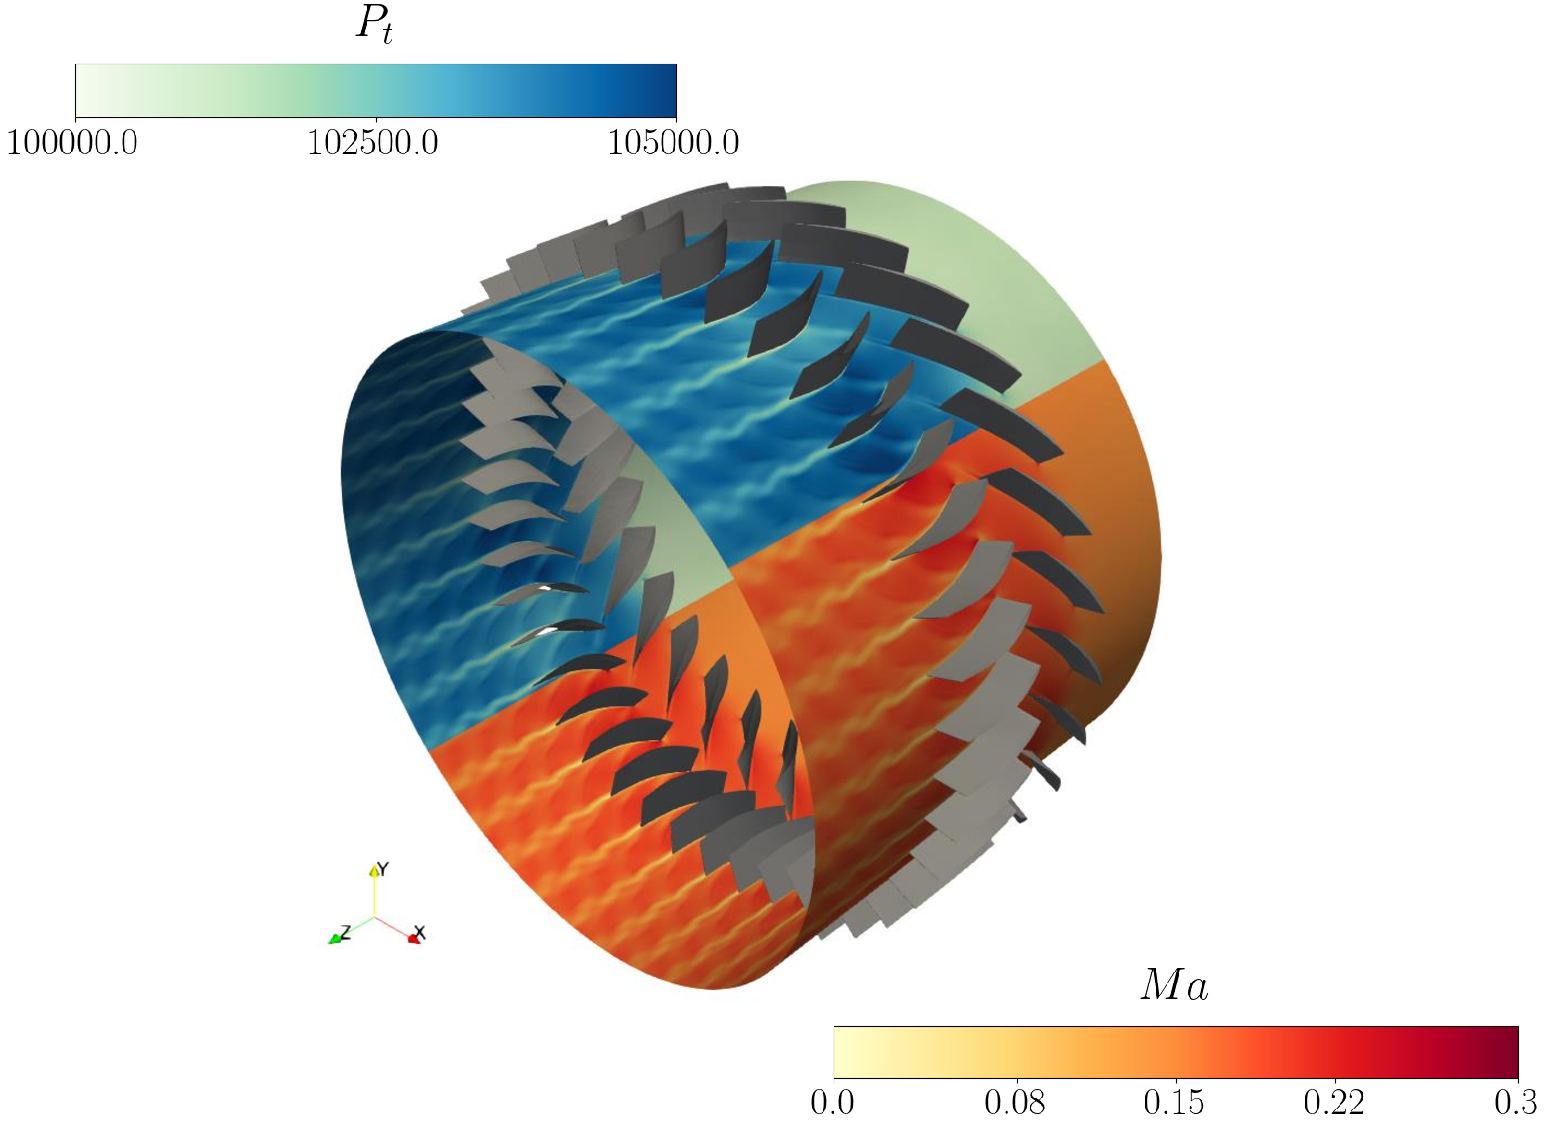
\includegraphics[scale=0.31]{../images/cme2.pdf}
                \scriptsize Simulation d'un écoulement dans un compresseur axial (CME2) \\ Tom MOUSSIE, LMFL - ENSAM
            \end{column}
            \begin{column}{0.45\textwidth}
                \textbf{Ouverture :} Combinaison de techniques expérimentales et numériques pour l'analyse des écoulements internes des compresseurs axiaux par assimilation de données

                \vspace{1cm}

                \textbf{Merci} pour votre attention !
            \end{column}
        \end{columns}
    \end{frame}
  


%\[
%\text{Coût de calcul} = 100\,\text{it} \times 35\,\text{membres} \times 127\,\text{cœurs} \times 0{,}33\,\text{it/h} \approx 150\,\text{kheures}
%\]

% --- Fin des slides principales ---
% Juste avant \appendix :
%\newcounter{mainframenumber}
%\setcounter{mainframenumber}{\value{framenumber}}


\appendix
%\renewcommand{\insertframenumber}{A\arabic{framenumber}}

\section*{Annexes}

% Figer le total au nombre de frames principales
%\setbeamertemplate{footline}{%
%  \hfill\\insertframenumber{} / \arabic{mainframenumber}\hspace{2ex}\vskip2pt
%}

% On remplace la numérotation normale par A1, A2, ...
%\renewcommand{\insertframenumber}{A\arabic{framenumber}}

\begin{frame}
  \frametitle{A1 : Ouverture}
  \begin{center}
    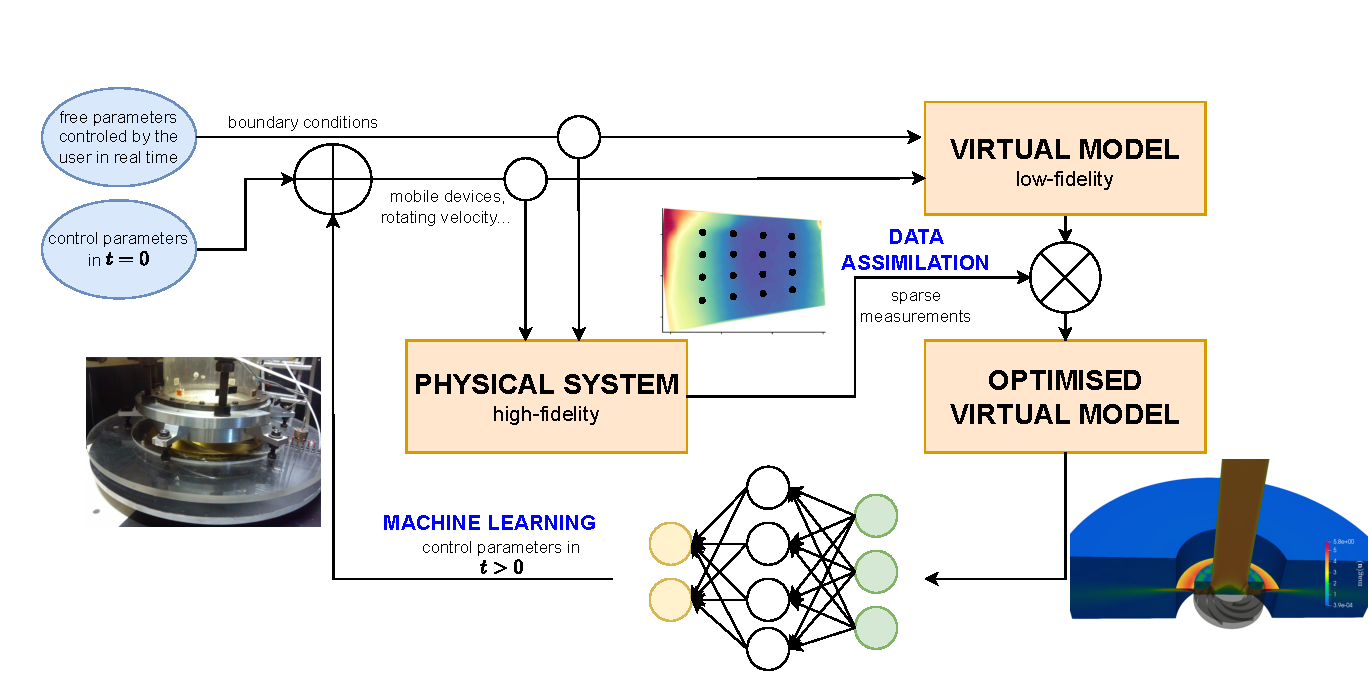
\includegraphics[scale=0.5]{../images/model/Digital_Twin_pump.pdf} \\
    \scriptsize Schéma du jumeau numérique de la pompe
  \end{center}
\end{frame}

\begin{frame}
  \frametitle{A2 : Profils de pression à l'entrée de la pompe}
  \begin{center}
    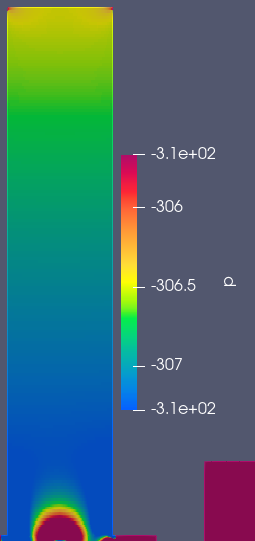
\includegraphics[scale=0.28]{../images/profil_pression_entrancePipe.png} \\
    \scriptsize Profil de pression à l'entrée de la pompe
  \end{center}
\end{frame}

\begin{frame}
  \frametitle{A3 : Autre résultat annexe}
  \begin{center}
    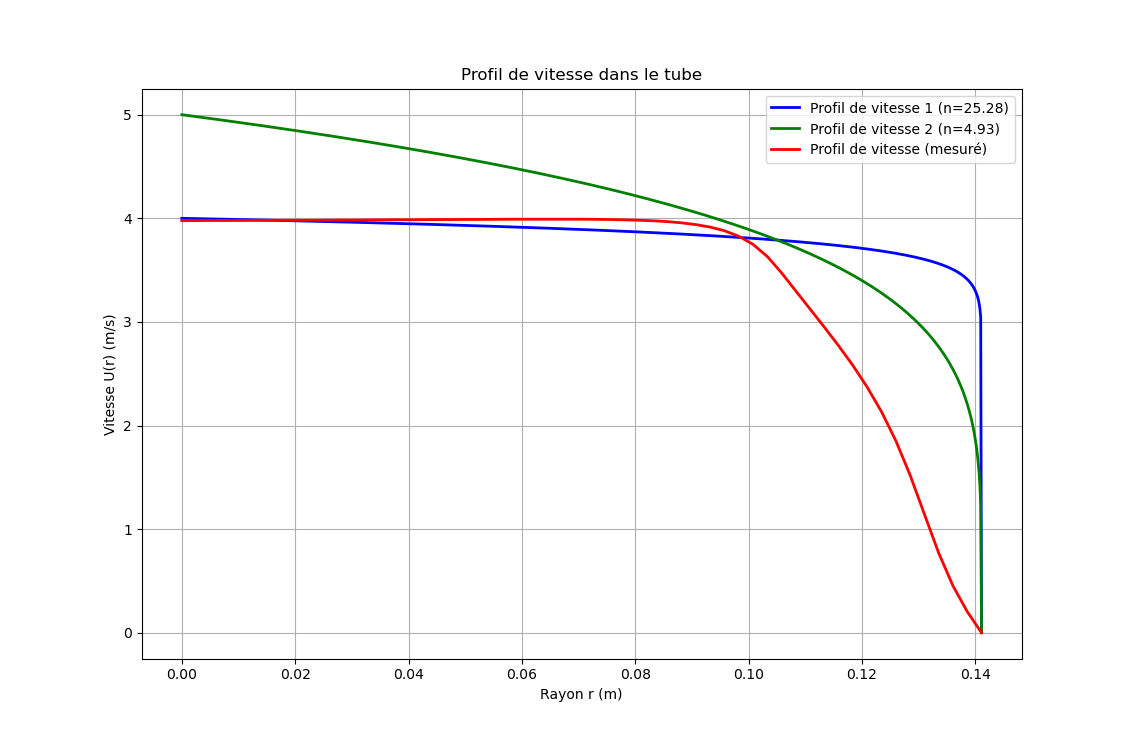
\includegraphics[scale=0.32]{../images/pv_x.png} \\
    \scriptsize Profil de pression analytique à l'entrée de la pompe
  \end{center}
\end{frame}

\begin{frame}
  \frametitle{A4 : Autre résultat annexe}
  \begin{center}
    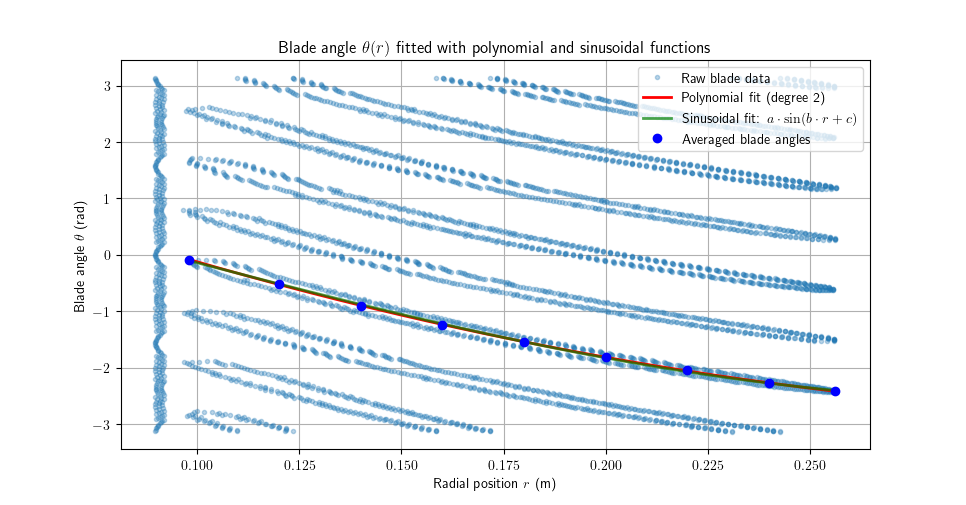
\includegraphics[scale=0.43]{../images/blade_interpolation_1.png} \\
    \scriptsize Interpolation des pales
  \end{center}
\end{frame}

\begin{frame}
  \frametitle{A5 : Autre résultat annexe}
  \begin{center}
    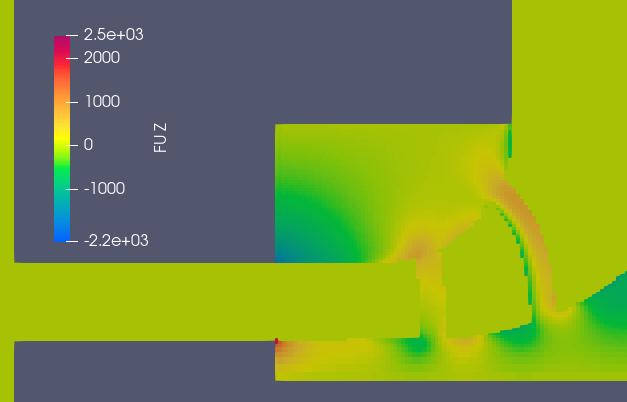
\includegraphics[scale=0.38]{../images/compensation_recirculation.png} \\
    \scriptsize Mise en valeur de l'effet de la méthode IBM
  \end{center}
\end{frame}

\begin{frame}
  \frametitle{A6 : Autre résultat annexe}
  \begin{center}
    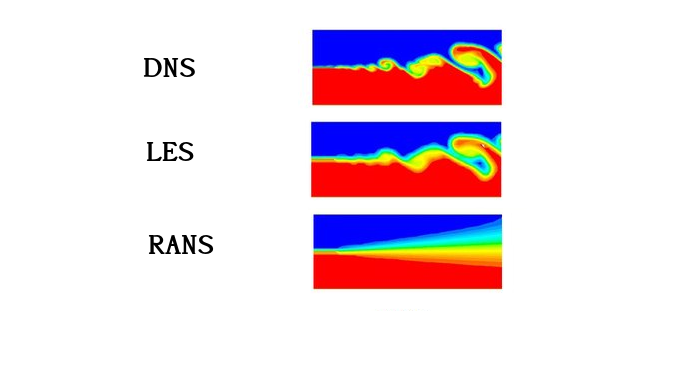
\includegraphics[scale=0.55]{../images/DNSLESRANS.png} \\
    \scriptsize Différence entre DNS, LES et RANS
  \end{center}
\end{frame}

\begin{frame}
  \frametitle{A7 : Autre résultat annexe}
  \begin{center}
    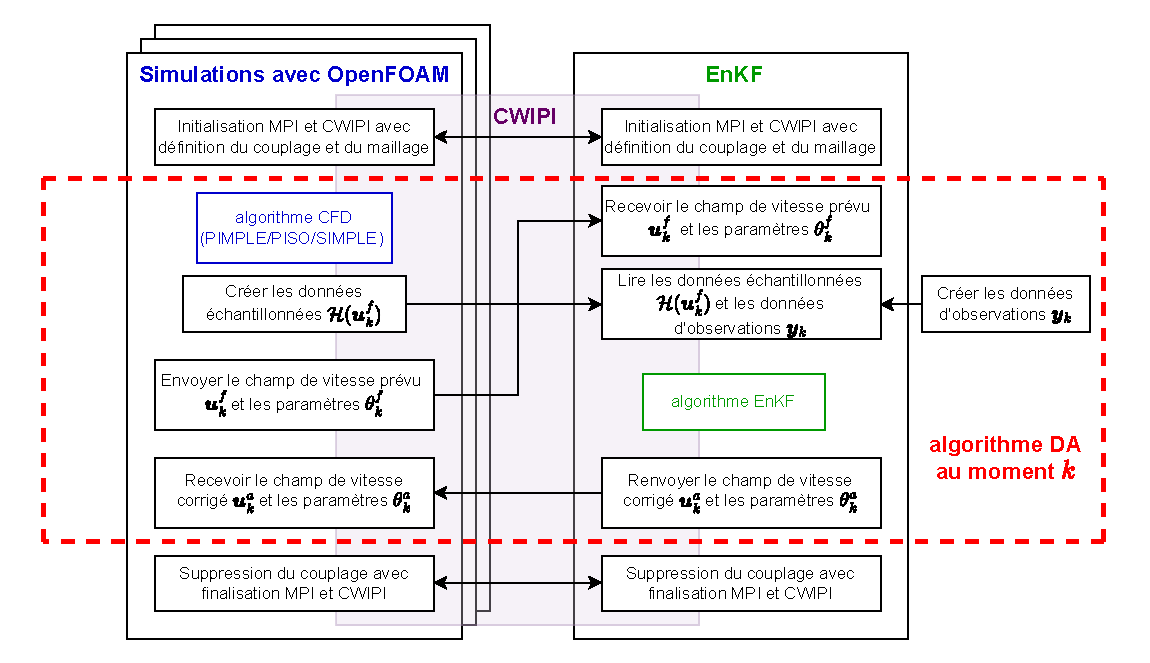
\includegraphics[scale=0.55]{../images/EnKF_Cones_français.pdf} \\
    \scriptsize Schéma détaillé de principe de CONES
  \end{center}
\end{frame}

\begin{frame}
  \frametitle{A8 : Autre résultat annexe}
  \begin{center}
    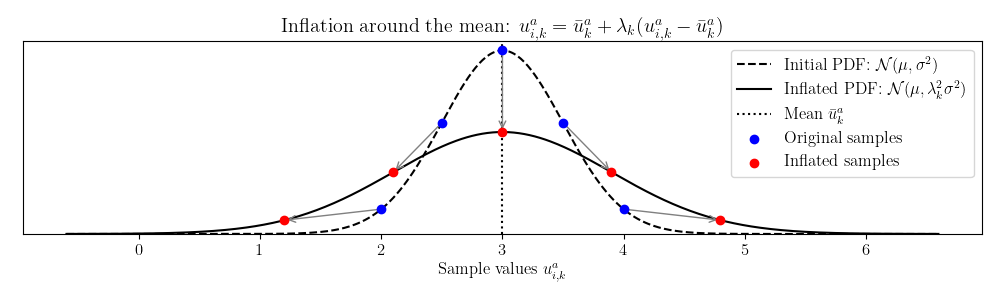
\includegraphics[scale=0.55]{../images/inflation.png} \\
    \scriptsize Schéma de principe de l'inflation codée dans CONES
  \end{center}
\end{frame}

\begin{frame}
  \frametitle{A9 : Autre résultat annexe}
  \begin{center}
    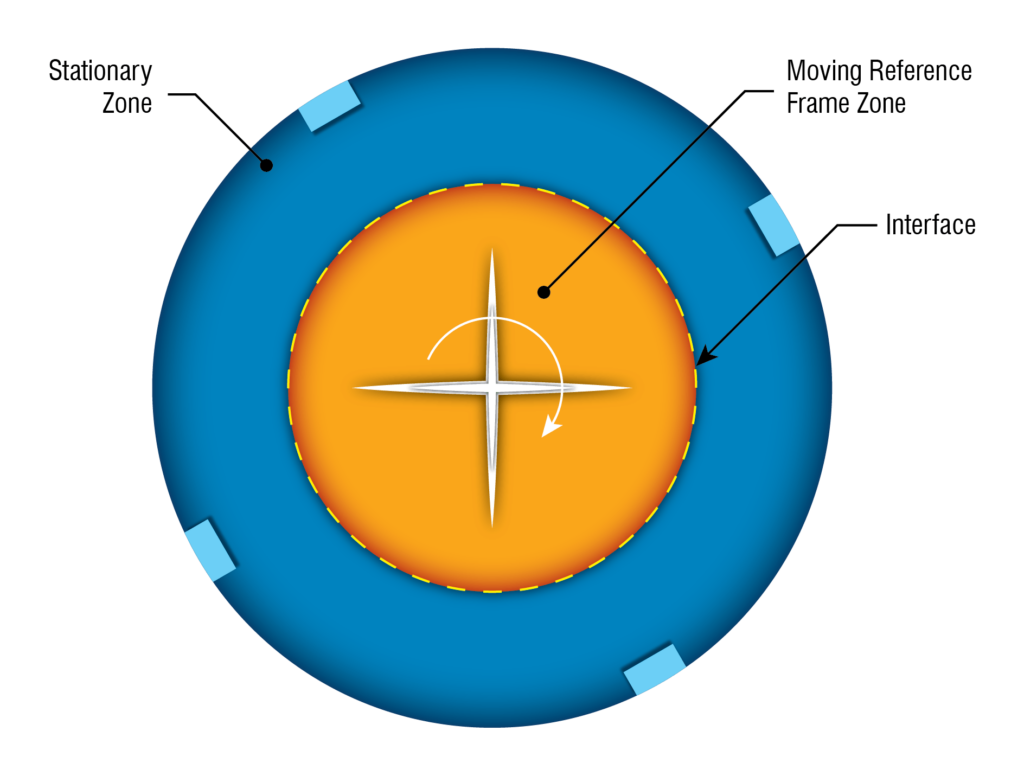
\includegraphics[scale=0.22]{../images/MRF.png} \\
    \scriptsize Schéma de principe de la méthode MRF
  \end{center}
\end{frame}

\begin{frame}
  \frametitle{A10 : Autre résultat annexe}
  \begin{center}
    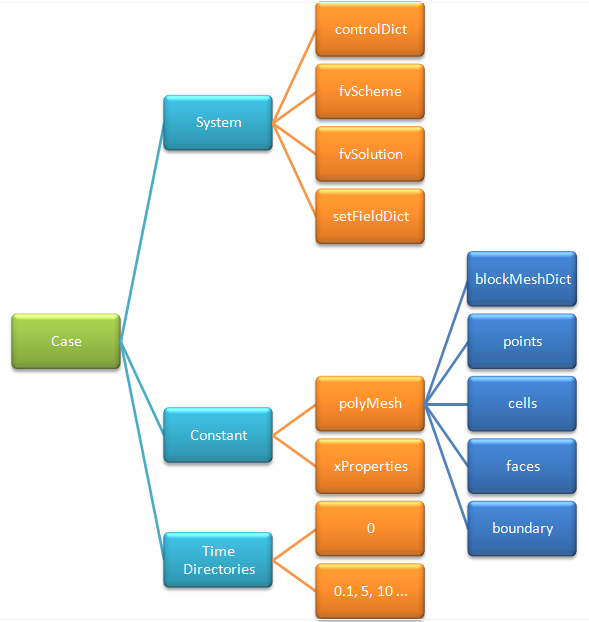
\includegraphics[scale=0.24]{../images/arborescence_of_2.png} \\
    \scriptsize Arborescence d'OpenFOAM
  \end{center}
\end{frame}

\begin{frame}
  \frametitle{A11 : Autre résultat annexe}
  \begin{center}
    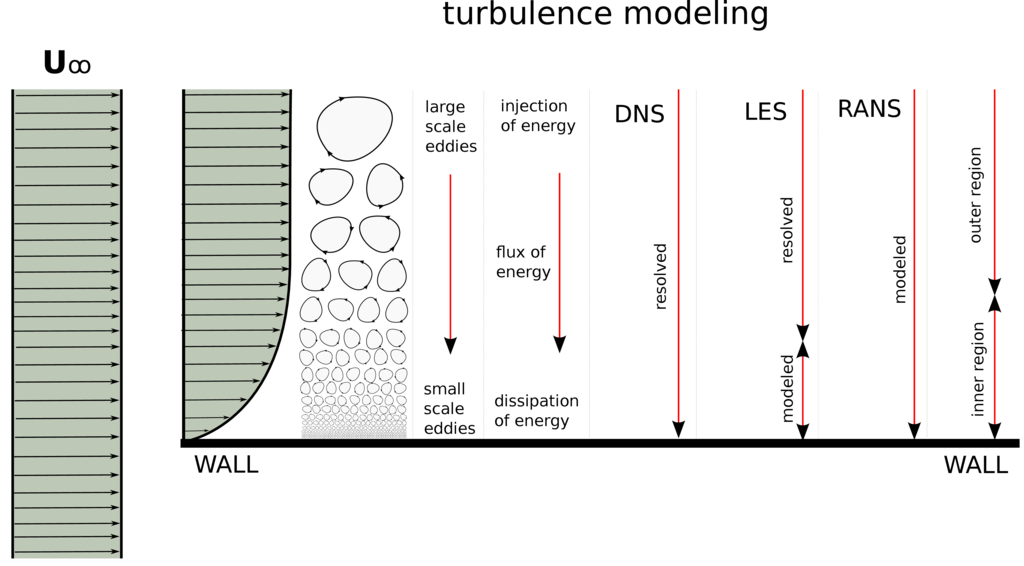
\includegraphics[scale=0.30]{../images/sketch-turbulent-flow-modeling-DNS-LES-RAS.png} \\
    \scriptsize DNS, LES et RANS
  \end{center}
\end{frame}

%\begin{frame}
%  \frametitle{A12 : Autre résultat annexe}
%  \begin{center}
%    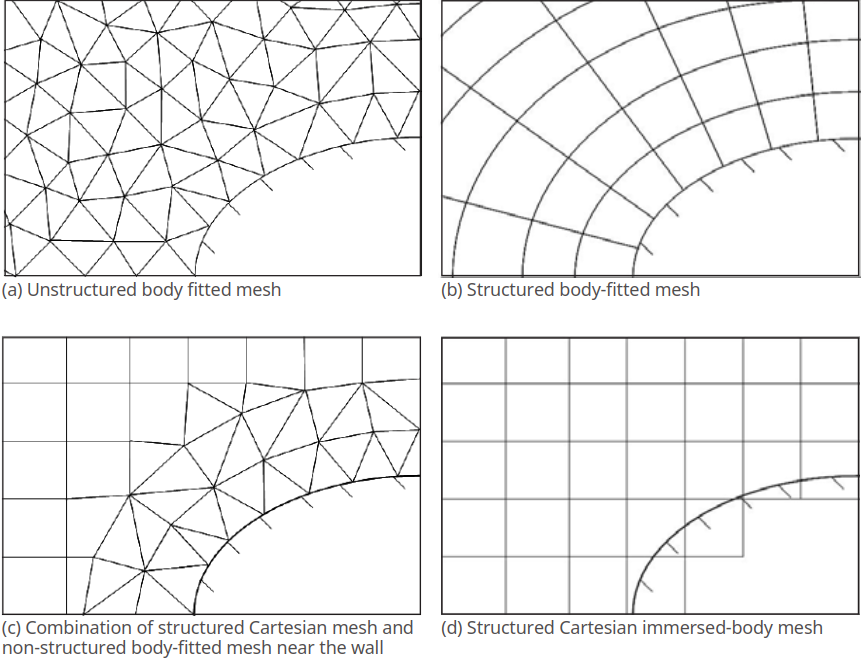
\includegraphics[scale=0.25]{../images/solidworksMesh3.png}
%  \end{center}
%\end{frame}

\begin{frame}
  \frametitle{A12 : Autre résultat annexe}
  \begin{center}
    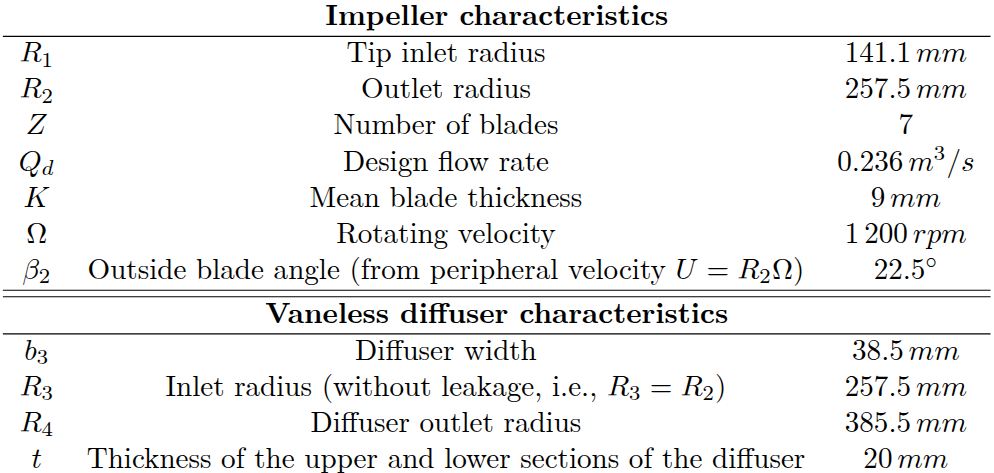
\includegraphics[scale=0.25]{../images/Tableau_caract.png}
  \end{center}
\end{frame}

\begin{frame}
  \frametitle{A13 : Autre résultat annexe}
  \begin{center}
    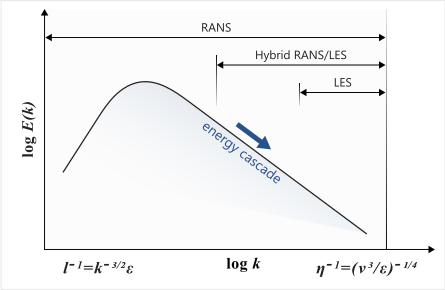
\includegraphics[scale=0.6]{../images/turbCascade.png}
  \end{center}
\end{frame}

\begin{frame}
  \frametitle{A14 : Autre résultat annexe}
  \begin{center}
    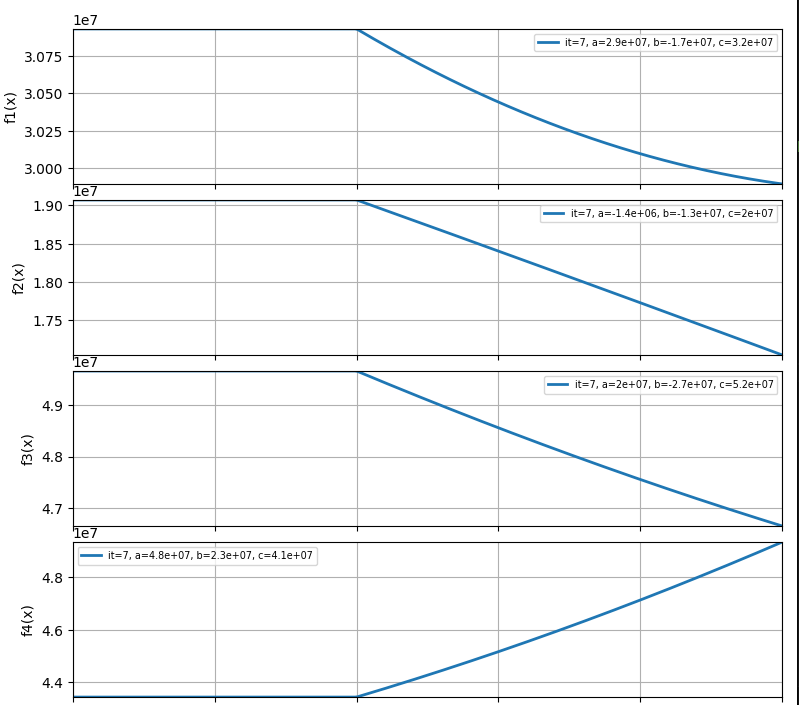
\includegraphics[scale=0.25]{../images/graph/radialExp.png}
  \end{center}
\end{frame}

\begin{frame}
  \frametitle{A15 : Jumeau numérique}
  \begin{center}
    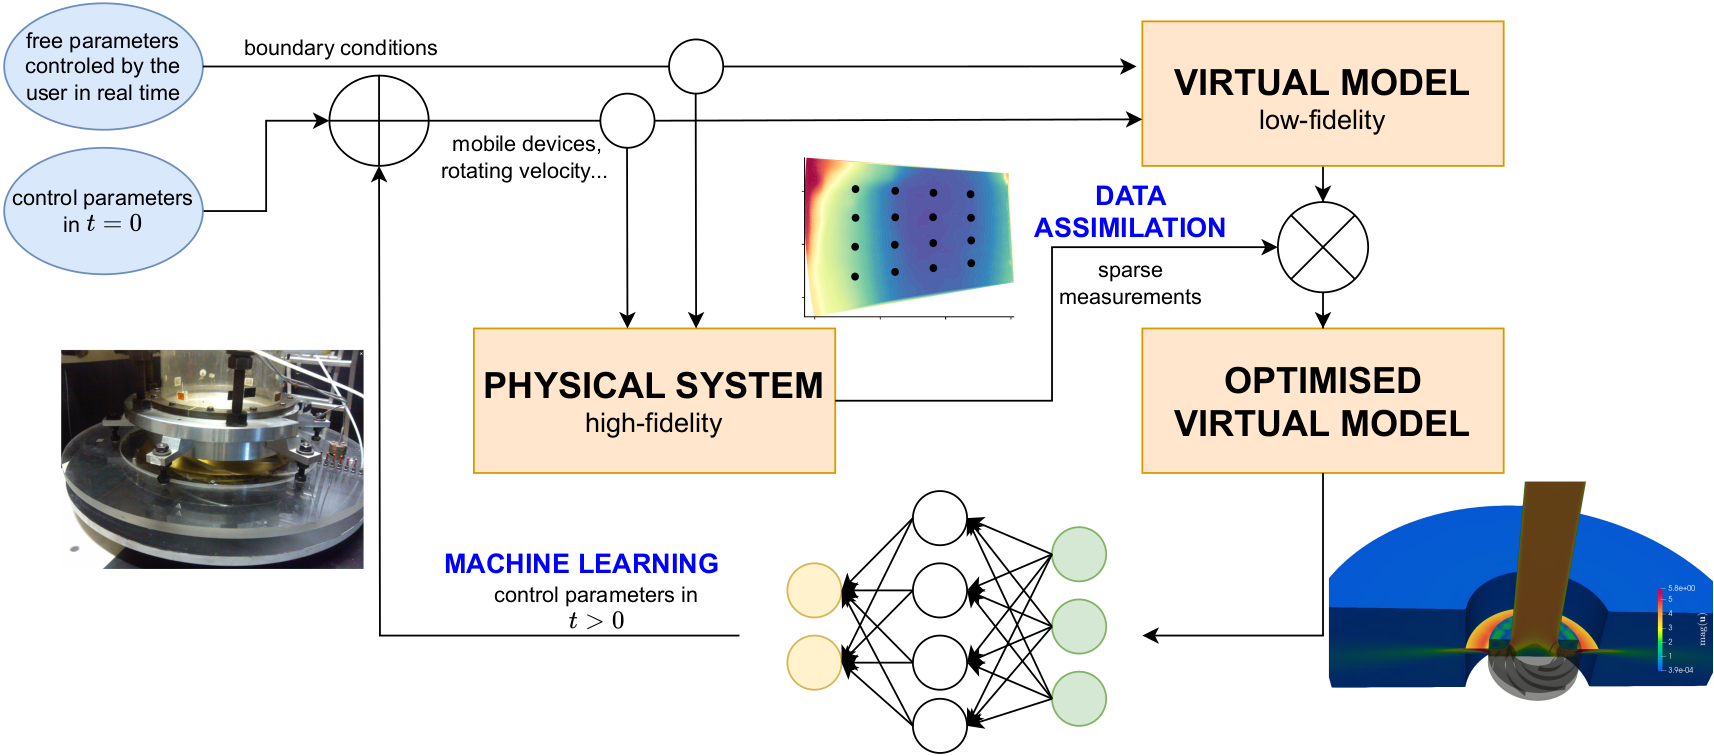
\includegraphics[scale=0.21]{../images/model/DigitalTwin.png}
  \end{center}
\end{frame}

\begin{frame}
  \frametitle{A16 : Roue}
  \begin{center}
    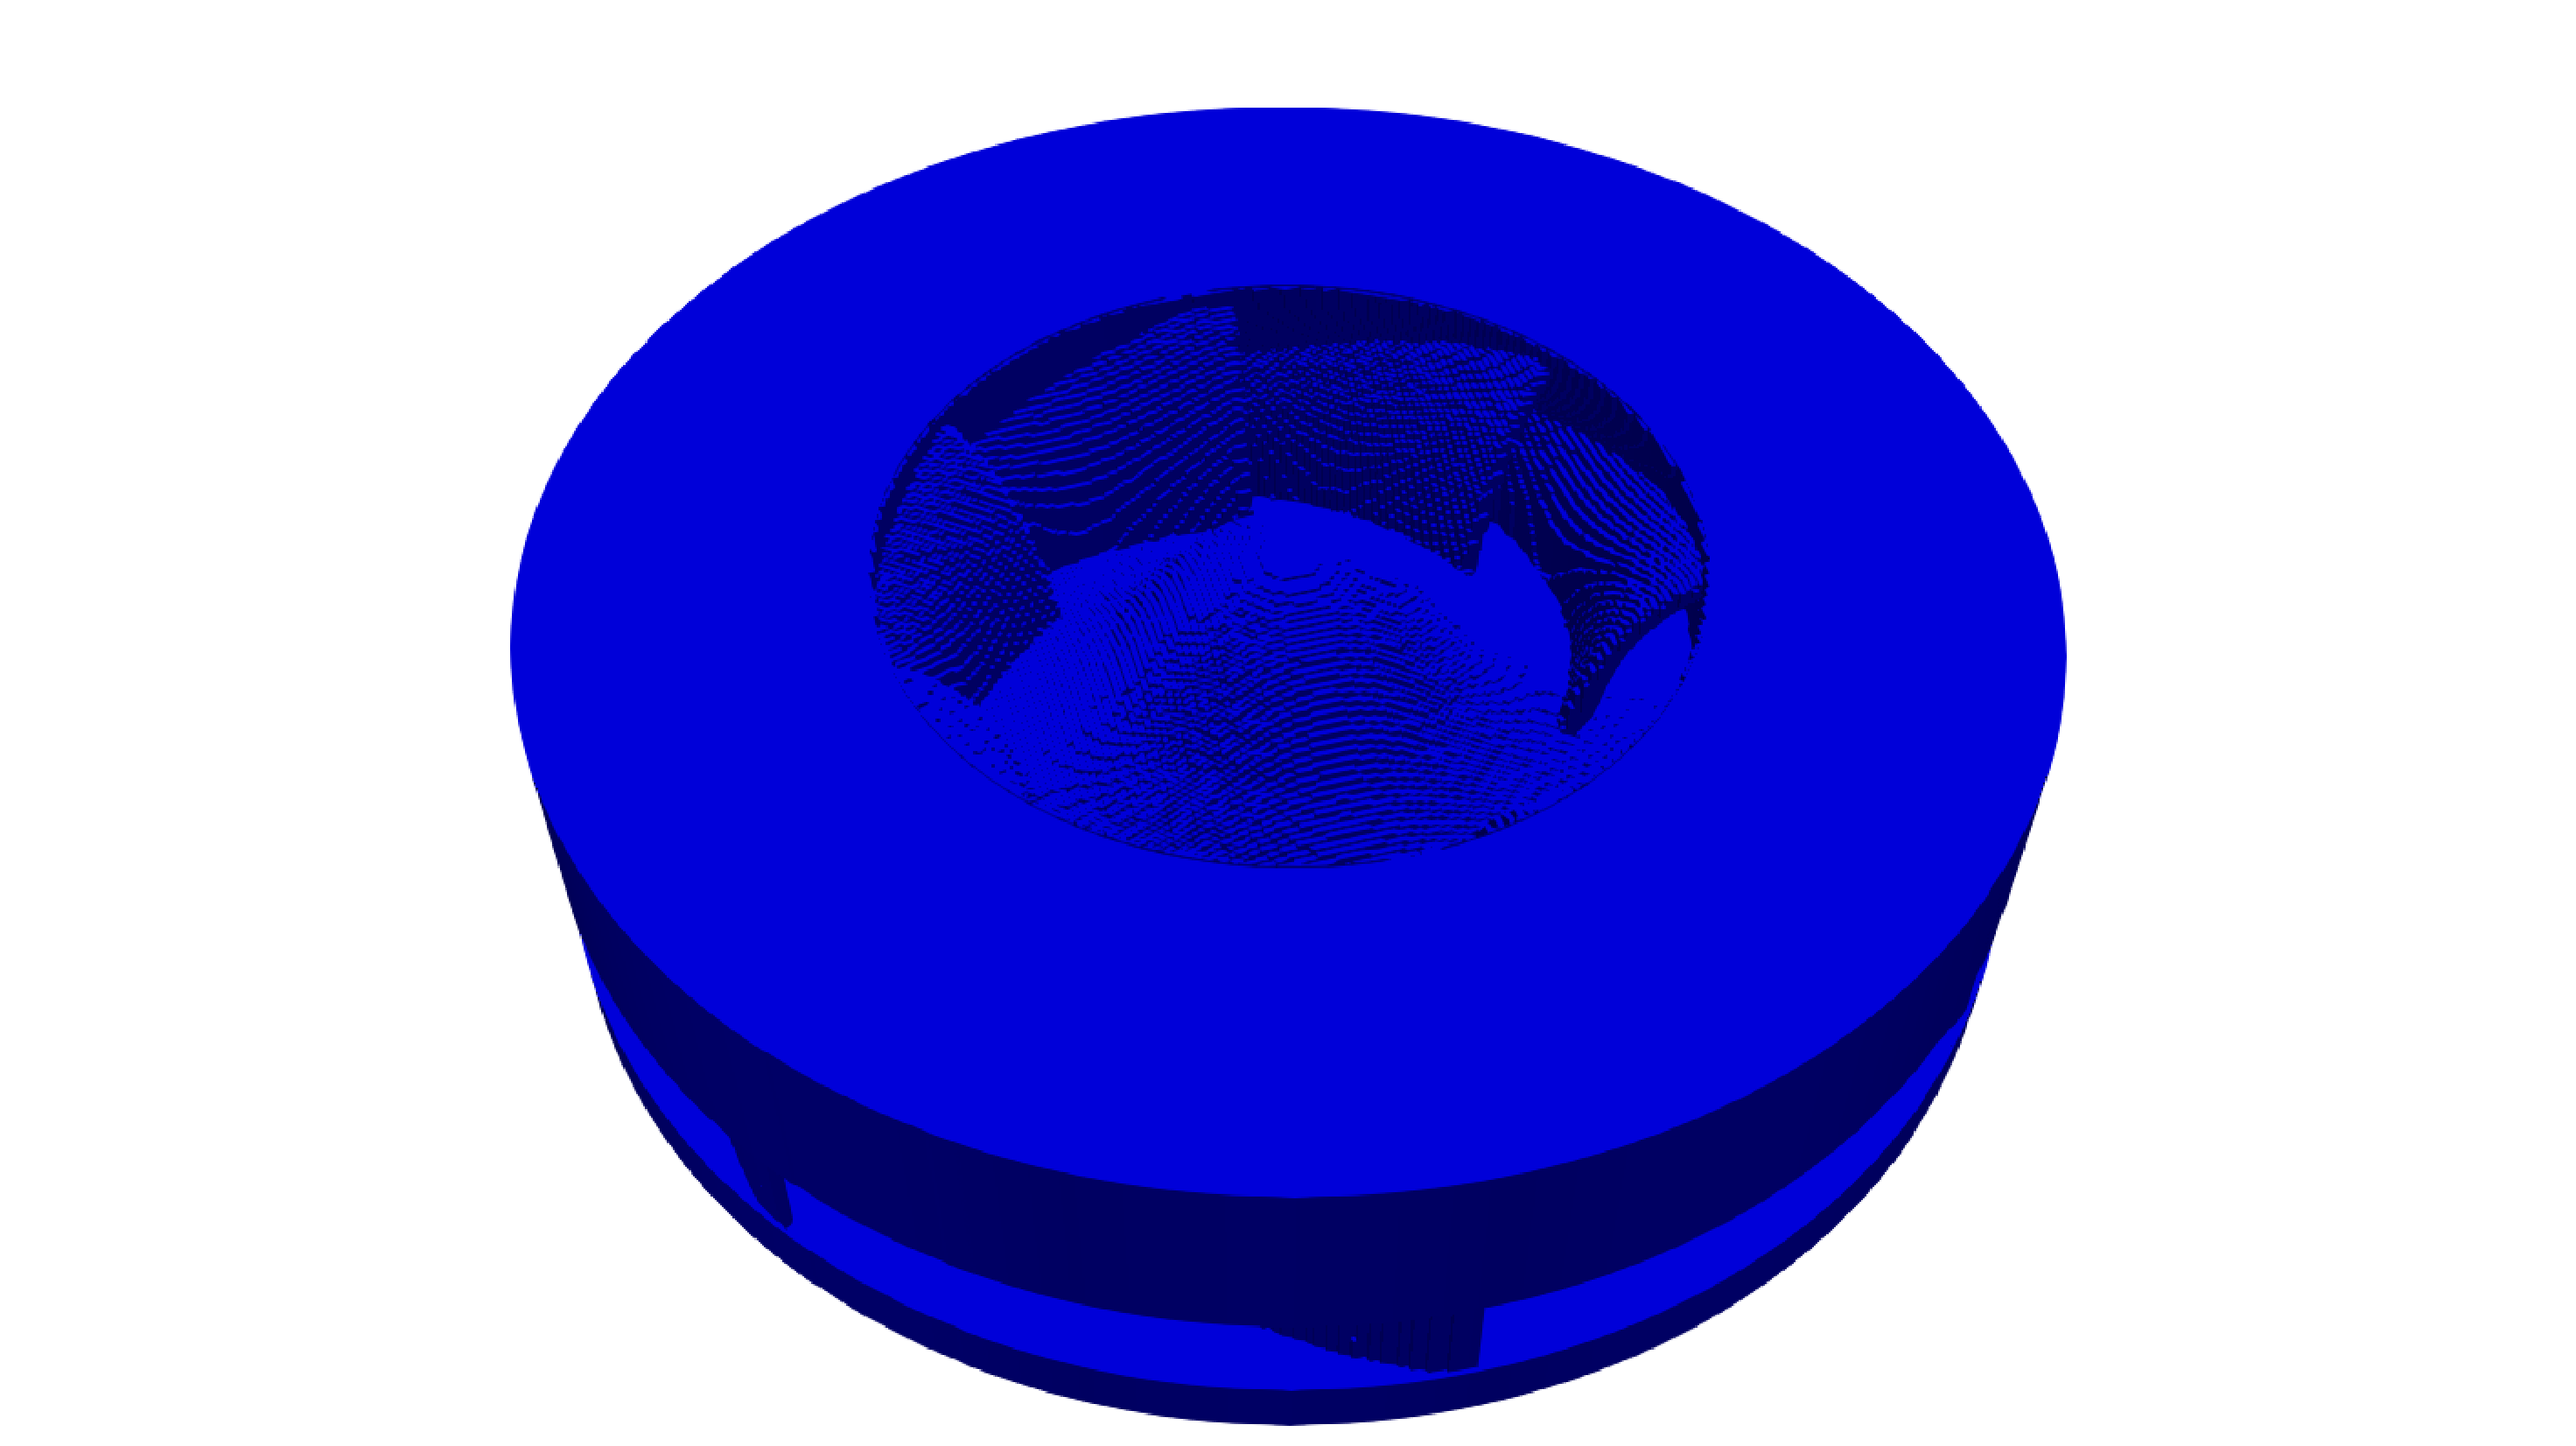
\includegraphics[scale=0.23]{../images/numericalPump/impeller_cells.pdf}
  \end{center}
\end{frame}

\begin{frame}
  \frametitle{A17 : Carte de la DA}
  \begin{center}
    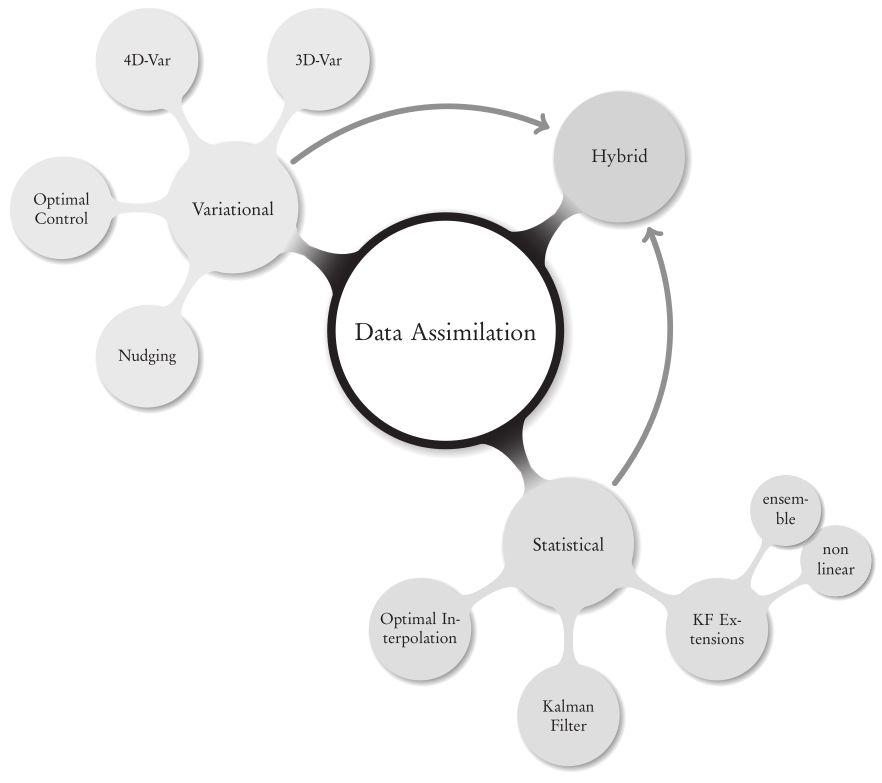
\includegraphics[scale=0.24]{../images/other/DAmap.png}
  \end{center}
\end{frame}

\begin{frame}
  \frametitle{A18 : Maillage}
  \begin{center}
    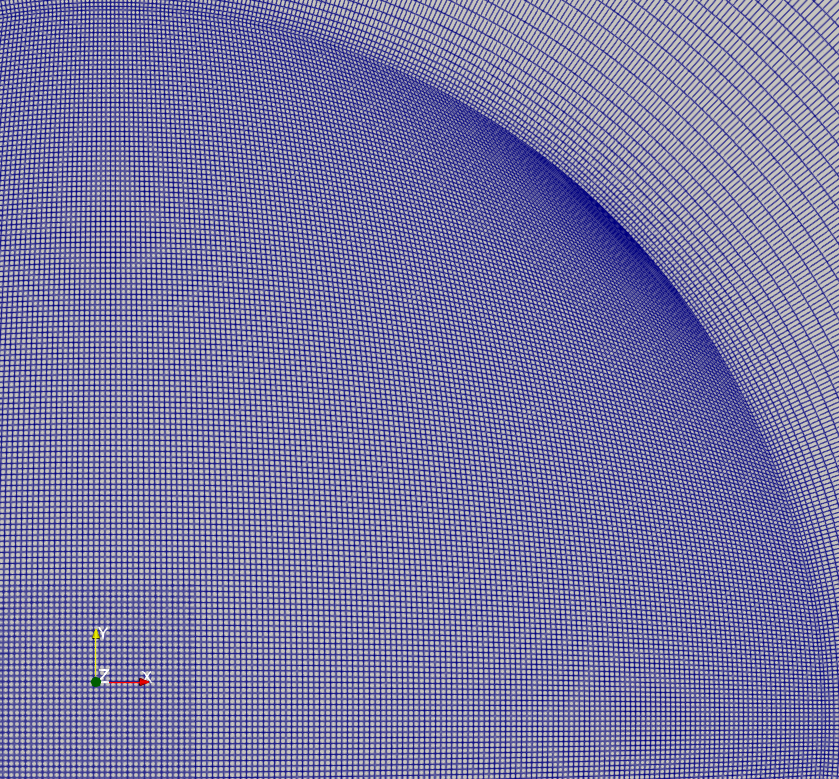
\includegraphics[scale=0.22]{../images/numericalPump/mesh.png}
  \end{center}
\end{frame}

\begin{frame}
  \frametitle{A19 : Modélisation proche paroi}
  \begin{center}
    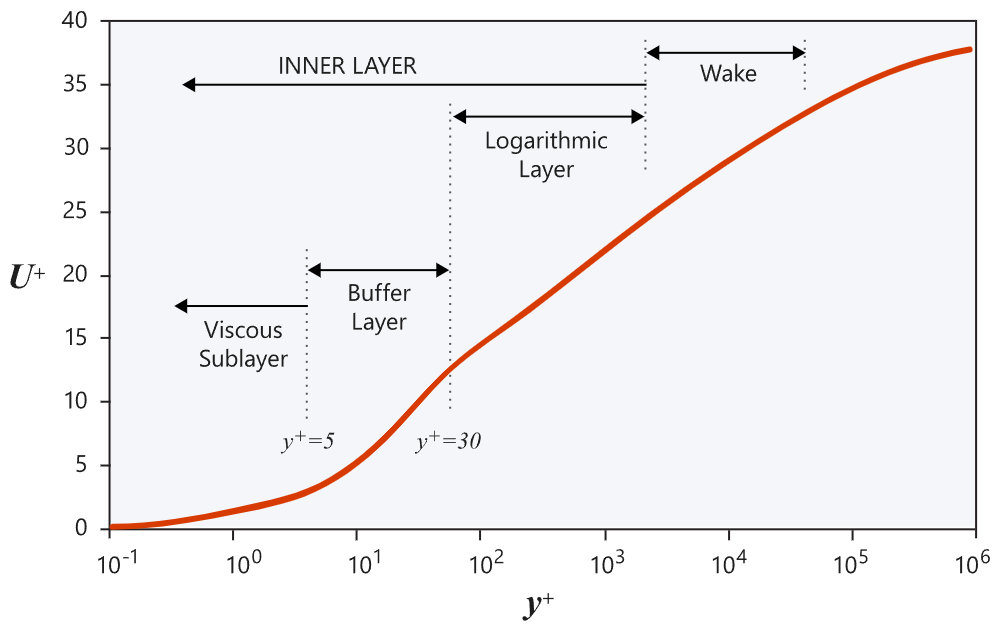
\includegraphics[scale=0.25]{../images/NearWallModelling.png}
  \end{center}
\end{frame}

\begin{frame}
  \frametitle{A20 : Penalisation IBM nulle}
  \begin{center}
    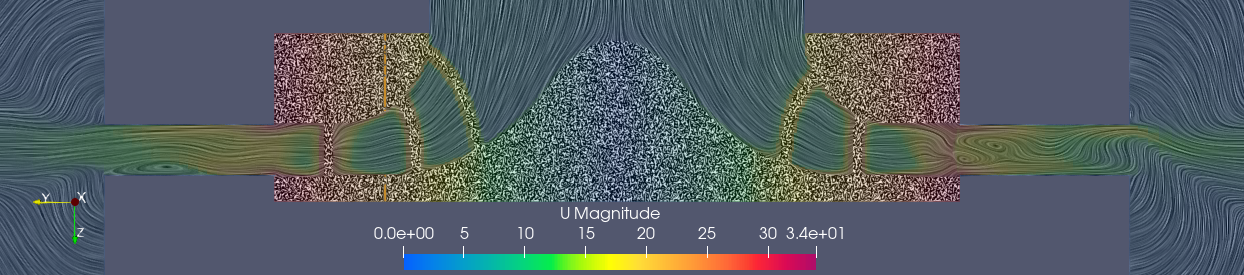
\includegraphics[scale=0.30]{../newFigures/pen0.png}
  \end{center}
\end{frame}

\end{document}


%\begin{figure}
%    \centering
%    
\includegraphics[width=0.5\linewidth]{recirculationBuble.png}
%    \caption{Enter Caption}
%    \label{fig:enter-label}
%\end{figure}